\chapter{Resultados de las Otras Series Reales}
\label{aneD_00_00_otras_series}

% Cinco series sin comportamientos (K = 1 en 99.5-100 % del test): corridas 103-107, M_ref = 10, test, w = 30.
% Mismas tablas que el Capítulo 4, con estas series; las figuras vienen de reports/reales/<serie>_m10/.

\providecommand{\figapl}[1]{\IfFileExists{#1}{\includegraphics[width=\textwidth]{#1}}%
{\fbox{\parbox{0.9\textwidth}{\centering\small Figura pendiente: \detokenize{#1}}}}}

\section{Series y diseño}
\label{aneD_00_01_series}
% Misma configuración que el tráfico (B-spline 10/3, FPCA en train, scores crudos, chungEscG, atau = 2, una cadena,
% rezagos cruzados con un rezago). Fuente de cada serie: 01 de cada corrida. Falta G, T y fuente exacta.

\begin{table}[H]
\centering\small
\caption{Series. Orígenes de prueba y ventana de detalle de 10 días consecutivos.}
\label{tab:aneD_series}
\begin{tabular}{l c c p{0.45\textwidth}}
\hline
Serie & Corrida & Orígenes de prueba & Criterio de la ventana de detalle (valor) \\
\hline
Precio SA1 (AEMO)             & 103 & 365  & Días con pico, RRP máximo $> 300$ AUD/MWh, $t = 1227..1236$ (9) \\
PM2.5 Parque O'Higgins        & 104 & 1096 & Días sobre la norma diaria, $\ge 50\ \mu$g/m$^3$, $t = 3474..3483$ (8) \\
PM2.5 Beijing (promedio PRSA) & 105 & 439  & Días con episodio severo, $\ge 150\ \mu$g/m$^3$, $t = 1400..1409$ (9) \\
Factor de planta eólico (SMARD) & 106 & 1290 & Días de temporal, factor medio $\ge 0.5$, $t = 3272..3281$ (10) \\
Volatilidad realizada BTCUSDT & 107 & 731  & Días turbulentos, log RV diaria $> -5.95$, $t = 1884..1893$ (3) \\
\hline
\end{tabular}
\end{table}

\section{Error puntual}
\label{aneD_00_02_error_puntual}

% Fuente: 98_resumen_bloqueA_min_max_prom.csv del _05 de cada serie.
\begin{table}[H]
\centering\small
\setlength{\tabcolsep}{3.5pt}
\caption{MAE y RMSE en el bloque de prueba por serie ($M = 10$, $w = 30$). En negrita el menor de cada fila.}
\label{tab:aneD_bloqueA}
\begin{tabular}{l ccccc ccccc}
\hline
 & \multicolumn{5}{c}{MAE} & \multicolumn{5}{c}{RMSE} \\
Serie & Esp. & Med. & Modal & RF & FAR & Esp. & Med. & Modal & RF & FAR \\
\hline
Precio SA1 & \textbf{0.328} & 0.329 & 0.344 & 0.341 & 0.328 & \textbf{0.442} & 0.443 & 0.467 & 0.453 & 0.442 \\
PM2.5 O'Higgins & \textbf{0.317} & 0.317 & 0.333 & 0.328 & 0.321 & \textbf{0.430} & 0.431 & 0.453 & 0.446 & 0.435 \\
PM2.5 Beijing & 0.566 & 0.552 & 0.579 & 0.596 & \textbf{0.551} & 0.745 & 0.750 & 0.838 & 0.761 & \textbf{0.739} \\
Eólica DE & 0.0859 & \textbf{0.0853} & 0.0993 & 0.0961 & 0.0857 & \textbf{0.1191} & 0.1196 & 0.1368 & 0.1270 & 0.1197 \\
BTC volatilidad & 0.329 & 0.330 & 0.349 & 0.329 & \textbf{0.324} & 0.423 & 0.425 & 0.447 & 0.423 & \textbf{0.418} \\
\hline
\end{tabular}
\end{table}

\begin{table}[H]
\centering\small
\setlength{\tabcolsep}{3.5pt}
\caption{Cambio relativo del MAE y del RMSE respecto del FAR por predictor y serie. Negativo es mejor que el FAR.}
\label{tab:aneD_bloqueA_ganancia}
\begin{tabular}{l cc cc cc cc}
\hline
 & \multicolumn{2}{c}{Esperanza} & \multicolumn{2}{c}{Mediana} & \multicolumn{2}{c}{Modal} & \multicolumn{2}{c}{RF} \\
Serie & MAE & RMSE & MAE & RMSE & MAE & RMSE & MAE & RMSE \\
\hline
Precio SA1 & $0.0\%$ & $0.0\%$ & $+0.2\%$ & $+0.3\%$ & $+4.8\%$ & $+5.6\%$ & $+4.1\%$ & $+2.5\%$ \\
PM2.5 O'Higgins & $-1.5\%$ & $-1.1\%$ & $-1.4\%$ & $-0.8\%$ & $+3.5\%$ & $+4.1\%$ & $+2.1\%$ & $+2.6\%$ \\
PM2.5 Beijing & $+2.9\%$ & $+0.7\%$ & $+0.2\%$ & $+1.5\%$ & $+5.1\%$ & $+13.5\%$ & $+8.2\%$ & $+2.9\%$ \\
Eólica DE & $+0.3\%$ & $-0.5\%$ & $-0.4\%$ & $-0.1\%$ & $+15.9\%$ & $+14.3\%$ & $+12.1\%$ & $+6.1\%$ \\
BTC volatilidad & $+1.4\%$ & $+1.1\%$ & $+1.9\%$ & $+1.5\%$ & $+7.6\%$ & $+6.7\%$ & $+1.5\%$ & $+1.1\%$ \\
\hline
\end{tabular}
\end{table}

% Fuente: 72_ventana_modelos_w30.csv (test, w = 30, sin el medoide).
\begin{table}[H]
\centering\small
\setlength{\tabcolsep}{3.5pt}
\caption{Ventanas de prueba ganadas por modelo, por MAE y por RMSE.}
\label{tab:aneD_bloqueA_ventanas}
\begin{tabular}{l ccccc ccccc}
\hline
 & \multicolumn{5}{c}{MAE} & \multicolumn{5}{c}{RMSE} \\
Serie & FAR & RF & Esp. & Med. & Modal & FAR & RF & Esp. & Med. & Modal \\
\hline
Precio SA1 & 45\% & 16\% & 23\% & 11\% & 4\% & 48\% & 25\% & 22\% & 4\% & 1\% \\
PM2.5 O'Higgins & 22\% & 17\% & 31\% & 26\% & 4\% & 25\% & 19\% & 28\% & 26\% & 1\% \\
PM2.5 Beijing & 40\% & 9\% & 5\% & 29\% & 19\% & 45\% & 14\% & 23\% & 17\% & 0\% \\
Eólica DE & 39\% & 4\% & 12\% & 40\% & 6\% & 34\% & 9\% & 23\% & 29\% & 5\% \\
BTC volatilidad & 52\% & 28\% & 17\% & 2\% & 1\% & 50\% & 32\% & 14\% & 3\% & 0\% \\
\hline
\end{tabular}
\end{table}

\begin{table}[H]
\centering\small
\setlength{\tabcolsep}{3.5pt}
\caption{Fracción de ventanas en que el predictor consistente del PSBPM-FD supera a cada referencia.}
\label{tab:aneD_bloqueA_gana}
\begin{tabular}{l cc cc}
\hline
 & \multicolumn{2}{c}{MAE (mediana)} & \multicolumn{2}{c}{RMSE (esperanza)} \\
Serie & vs FAR & vs RF & vs FAR & vs RF \\
\hline
Precio SA1 & 41\% & 82\% & 43\% & 74\% \\
PM2.5 O'Higgins & 69\% & 77\% & 67\% & 79\% \\
PM2.5 Beijing & 54\% & 86\% & 43\% & 74\% \\
Eólica DE & 55\% & 95\% & 56\% & 90\% \\
BTC volatilidad & 18\% & 46\% & 23\% & 52\% \\
\hline
\end{tabular}
\end{table}

\section{Intervalos de predicción}
\label{aneD_00_03_intervalos}

% Fuente: 99_resumen_bloqueB_min_max_prom.csv y 81_ventana_bloqueB_w30.csv.
\begin{table}[H]
\centering\small
\setlength{\tabcolsep}{3.5pt}
\caption{Winkler y MPIW en el bloque de prueba por serie y construcción ($M = 10$). En negrita el menor Winkler de cada fila.}
\label{tab:aneD_bloqueB_winkler}
\begin{tabular}{l cccc cccc}
\hline
 & \multicolumn{4}{c}{Winkler} & \multicolumn{4}{c}{MPIW} \\
Serie & FAR & Equi. & HDR & Simult. & FAR & Equi. & HDR & Simult. \\
\hline
Precio SA1 & 2.374 & \textbf{2.354} & 2.361 & 2.977 & 1.872 & 1.881 & 1.885 & 2.870 \\
PM2.5 O'Higgins & 2.484 & \textbf{2.421} & 2.441 & 2.696 & 1.645 & 1.692 & 1.687 & 2.450 \\
PM2.5 Beijing & 3.883 & \textbf{3.522} & 3.717 & 4.169 & 2.710 & 2.852 & 2.847 & 3.986 \\
Eólica DE & \textbf{0.581} & 0.605 & 0.622 & 0.730 & 0.454 & 0.488 & 0.487 & 0.674 \\
BTC volatilidad & \textbf{2.075} & 2.076 & 2.075 & 2.608 & 1.634 & 1.735 & 1.739 & 2.597 \\
\hline
\end{tabular}
\end{table}

\begin{table}[H]
\centering\small
\setlength{\tabcolsep}{3.5pt}
\caption{PICP y PICPB en el bloque de prueba por serie y construcción ($M = 10$). Nominal $0.95$.}
\label{tab:aneD_bloqueB_picp}
\begin{tabular}{l cccc cccc}
\hline
 & \multicolumn{4}{c}{PICP} & \multicolumn{4}{c}{PICPB} \\
Serie & FAR & Equi. & HDR & Simult. & FAR & Equi. & HDR & Simult. \\
\hline
Precio SA1 & 0.956 & 0.956 & 0.956 & 0.994 & 0.717 & 0.696 & 0.702 & 0.947 \\
PM2.5 O'Higgins & 0.937 & 0.942 & 0.941 & 0.981 & 0.676 & 0.686 & 0.696 & 0.901 \\
PM2.5 Beijing & 0.933 & 0.939 & 0.933 & 0.980 & 0.786 & 0.763 & 0.763 & 0.926 \\
Eólica DE & 0.946 & 0.955 & 0.956 & 0.985 & 0.783 & 0.808 & 0.825 & 0.940 \\
BTC volatilidad & 0.944 & 0.954 & 0.955 & 0.995 & 0.633 & 0.673 & 0.677 & 0.951 \\
\hline
\end{tabular}
\end{table}

\begin{table}[H]
\centering\small
\setlength{\tabcolsep}{3pt}
\caption{Cambio relativo del Winkler y del MPIW respecto del FAR por serie y construcción. Negativo es mejor que el FAR.}
\label{tab:aneD_bloqueB_ganancia}
\begin{tabular}{l cc cc cc}
\hline
 & \multicolumn{2}{c}{Equi-colas} & \multicolumn{2}{c}{Máxima densidad} & \multicolumn{2}{c}{Simultánea} \\
Serie & Winkler & MPIW & Winkler & MPIW & Winkler & MPIW \\
\hline
Precio SA1 & $-0.8\%$ & $+0.5\%$ & $-0.5\%$ & $+0.7\%$ & $+25.4\%$ & $+53.3\%$ \\
PM2.5 O'Higgins & $-2.5\%$ & $+2.9\%$ & $-1.7\%$ & $+2.5\%$ & $+8.5\%$ & $+48.9\%$ \\
PM2.5 Beijing & $-9.3\%$ & $+5.3\%$ & $-4.3\%$ & $+5.1\%$ & $+7.4\%$ & $+47.1\%$ \\
Eólica DE & $+4.2\%$ & $+7.5\%$ & $+7.0\%$ & $+7.2\%$ & $+25.7\%$ & $+48.5\%$ \\
BTC volatilidad & $+0.1\%$ & $+6.2\%$ & $+0.0\%$ & $+6.4\%$ & $+25.7\%$ & $+59.0\%$ \\
\hline
\end{tabular}
\end{table}

\begin{table}[H]
\centering\small
\setlength{\tabcolsep}{3.5pt}
\caption{Ventanas de prueba ganadas por Winkler.}
\label{tab:aneD_bloqueB_ventanas}
\begin{tabular}{l cccc ccc}
\hline
 & \multicolumn{4}{c}{La mejor banda} & \multicolumn{3}{c}{Gana al FAR} \\
Serie & FAR & Equi. & HDR & Simult. & Equi. & HDR & Simult. \\
\hline
Precio SA1 & 39\% & 35\% & 19\% & 7\% & 60\% & 52\% & 8\% \\
PM2.5 O'Higgins & 32\% & 35\% & 16\% & 17\% & 61\% & 57\% & 24\% \\
PM2.5 Beijing & 20\% & 78\% & 3\% & 0\% & 80\% & 68\% & 28\% \\
Eólica DE & 64\% & 20\% & 16\% & 1\% & 34\% & 30\% & 1\% \\
BTC volatilidad & 53\% & 25\% & 21\% & 0\% & 44\% & 42\% & 2\% \\
\hline
\end{tabular}
\end{table}

\section{Comportamientos}
\label{aneD_00_04_comportamientos}

% Fuente: 102_K_por_M.csv del barrido de cada serie. Con K = 1 el pronóstico por comportamiento es la esperanza.
\begin{table}[H]
\centering\small
\setlength{\tabcolsep}{3.5pt}
\caption{Distribución de $K_t$ en el bloque de prueba por serie ($M = 10$).}
\label{tab:aneD_K}
\begin{tabular}{l c ccc}
\hline
Serie & Orígenes & $K_t = 1$ & $K_t = 2$ & $K_t \ge 3$ \\
\hline
Precio SA1 & 365 & 99.7\% & 0.3\% & 0.0\% \\
PM2.5 O'Higgins & 1096 & 99.5\% & 0.5\% & 0.0\% \\
PM2.5 Beijing & 439 & 100.0\% & 0.0\% & 0.0\% \\
Eólica DE & 1290 & 99.9\% & 0.1\% & 0.0\% \\
BTC volatilidad & 731 & 100.0\% & 0.0\% & 0.0\% \\
\hline
\end{tabular}
\end{table}

\section{Figuras por serie}
\label{aneD_00_05_figuras}

\subsection{Precio SA1 (AEMO)}
\label{aneD_00_05_103}

\begin{figure}[H]
\centering
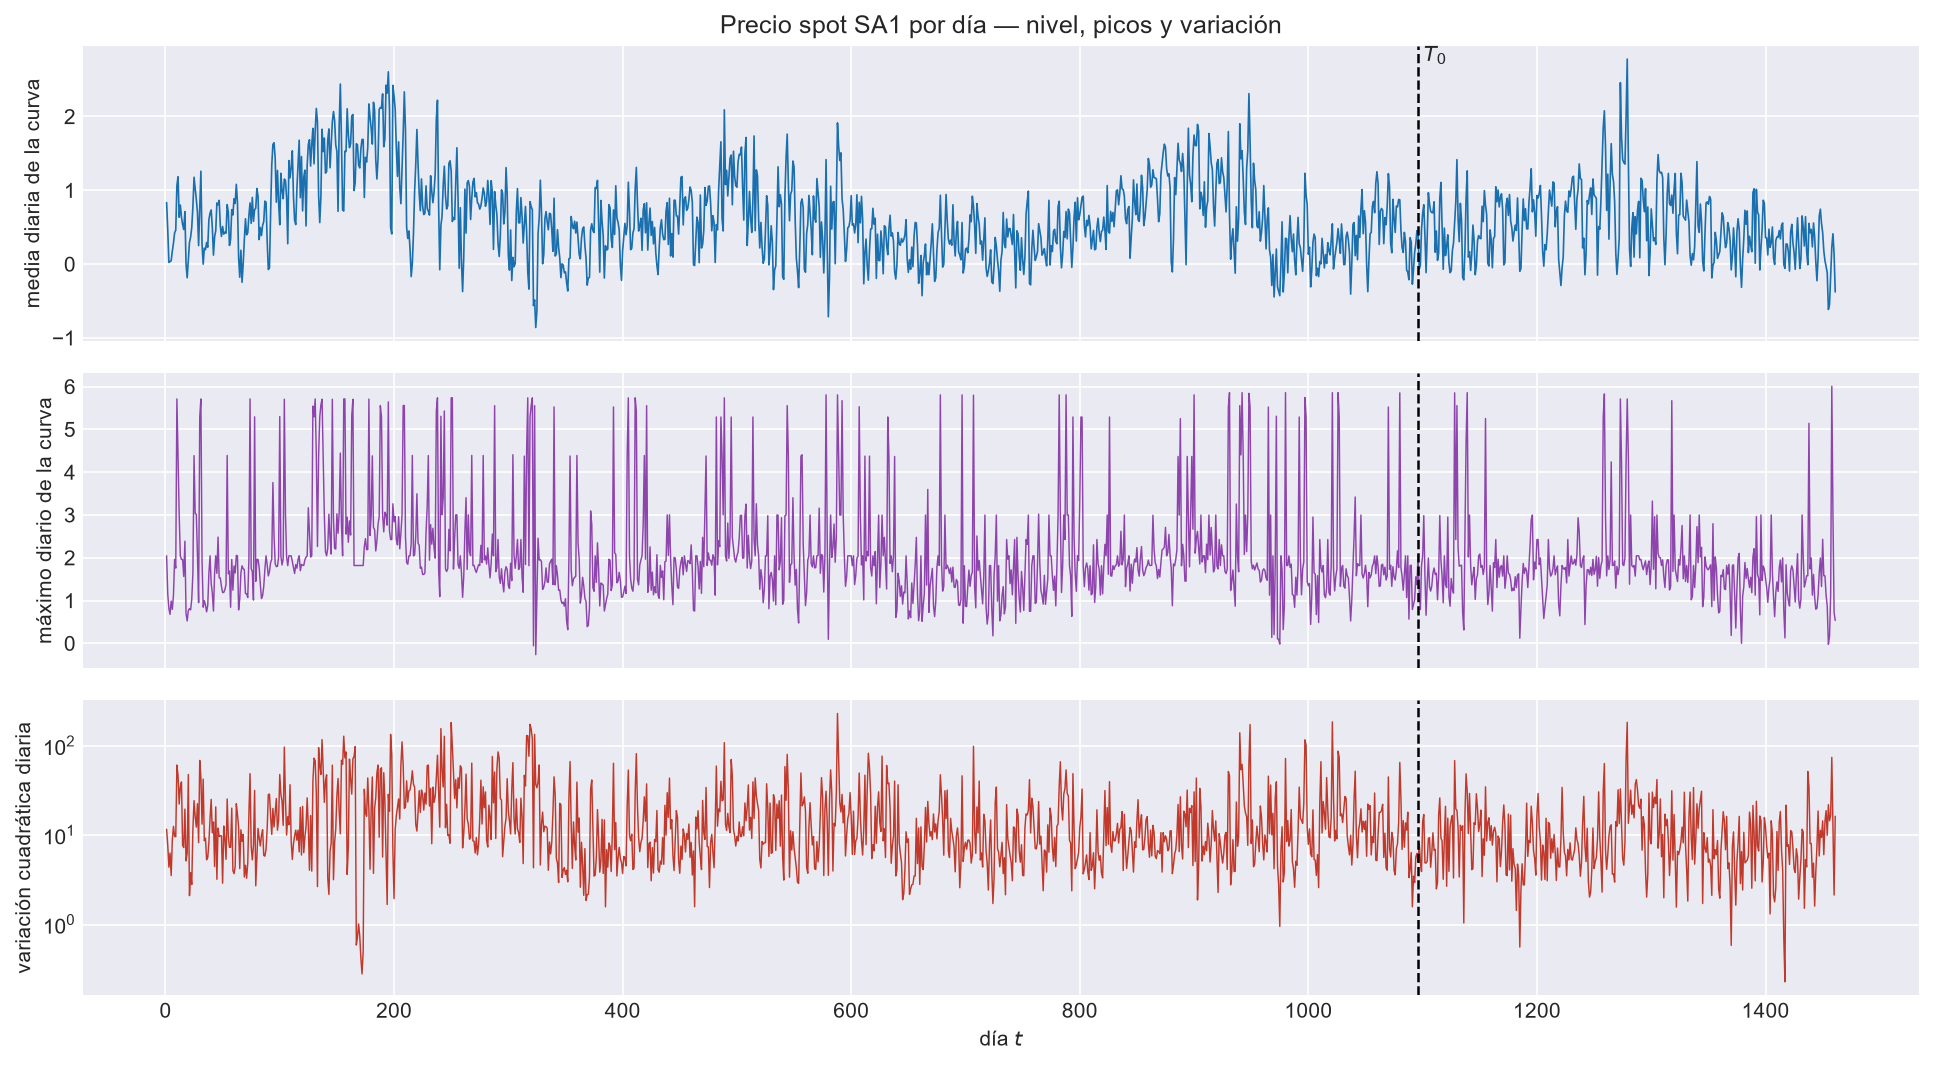
\includegraphics[width=\textwidth,height=0.75\textheight,keepaspectratio]{IMG/aneD_00/aneD_00_04_serie_diaria_103.png}
\caption{Precio SA1 (AEMO). Serie diaria.}
\label{fig:aneD_04_serie_diaria_103}
\end{figure}

\begin{figure}[H]
\centering
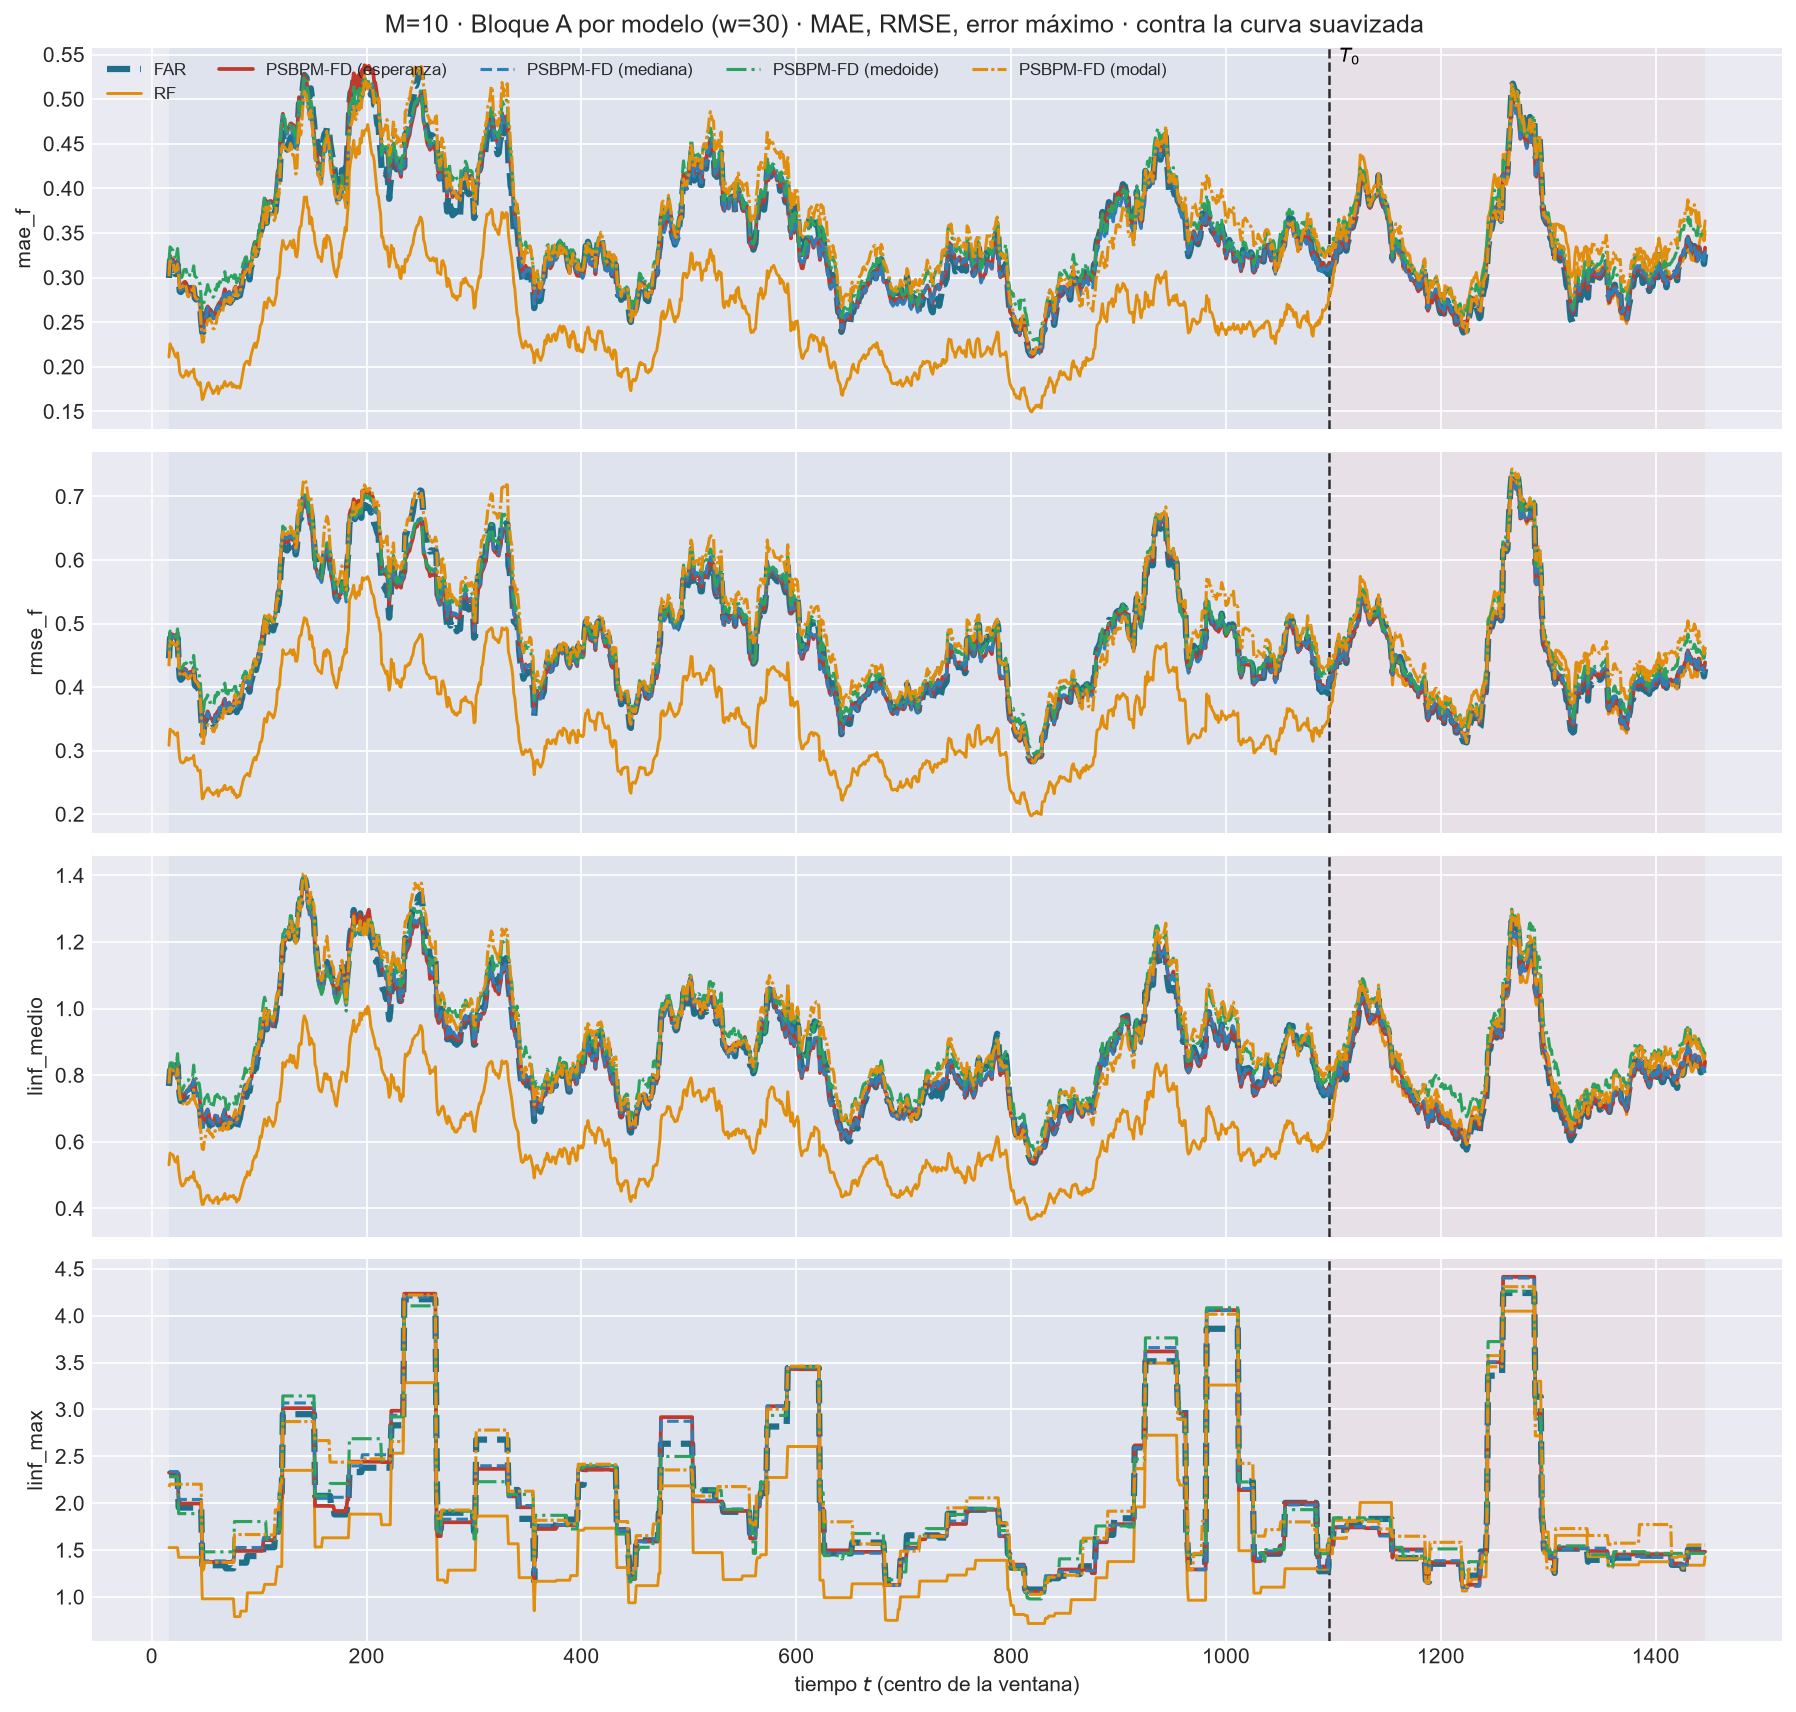
\includegraphics[width=\textwidth,height=0.75\textheight,keepaspectratio]{IMG/aneD_00/aneD_00_78_ventana_bloqueA_modelos_w30_103.png}
\caption{Precio SA1 (AEMO). MAE sobre la ventana móvil del bloque de prueba ($M = 10$, $w = 30$).}
\label{fig:aneD_78_ventana_bloqueA_modelos_w30_103}
\end{figure}

\begin{figure}[H]
\centering
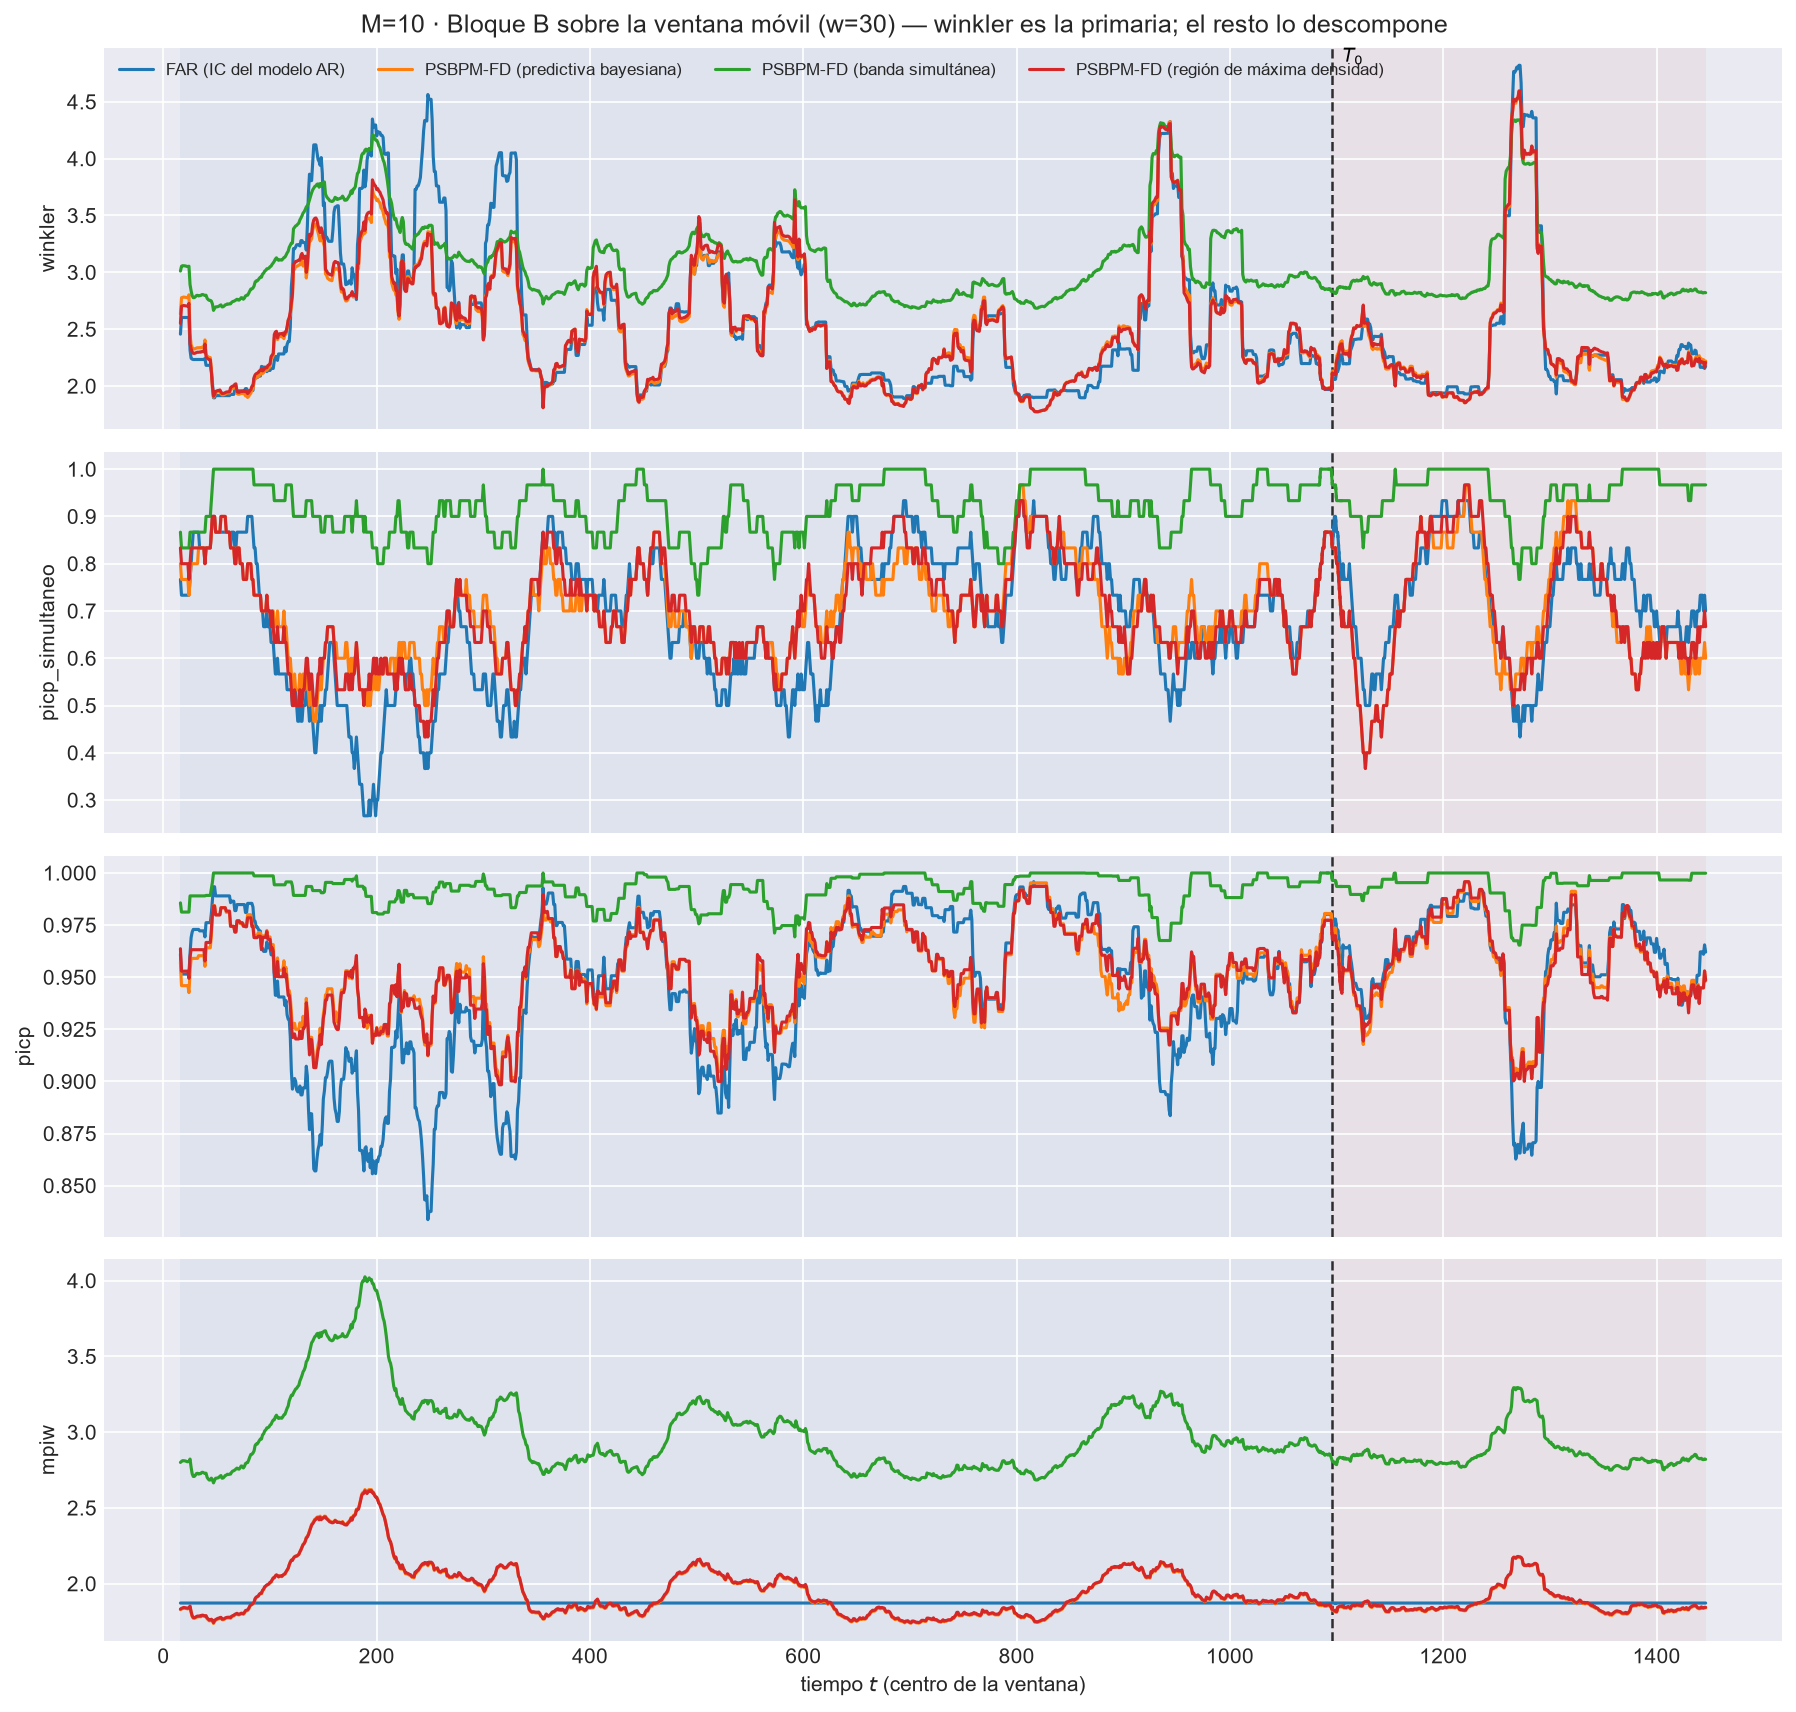
\includegraphics[width=\textwidth,height=0.75\textheight,keepaspectratio]{IMG/aneD_00/aneD_00_81_ventana_bloqueB_w30_103.png}
\caption{Precio SA1 (AEMO). Winkler sobre la ventana móvil del bloque de prueba ($M = 10$, $w = 30$).}
\label{fig:aneD_81_ventana_bloqueB_w30_103}
\end{figure}

\begin{figure}[H]
\centering
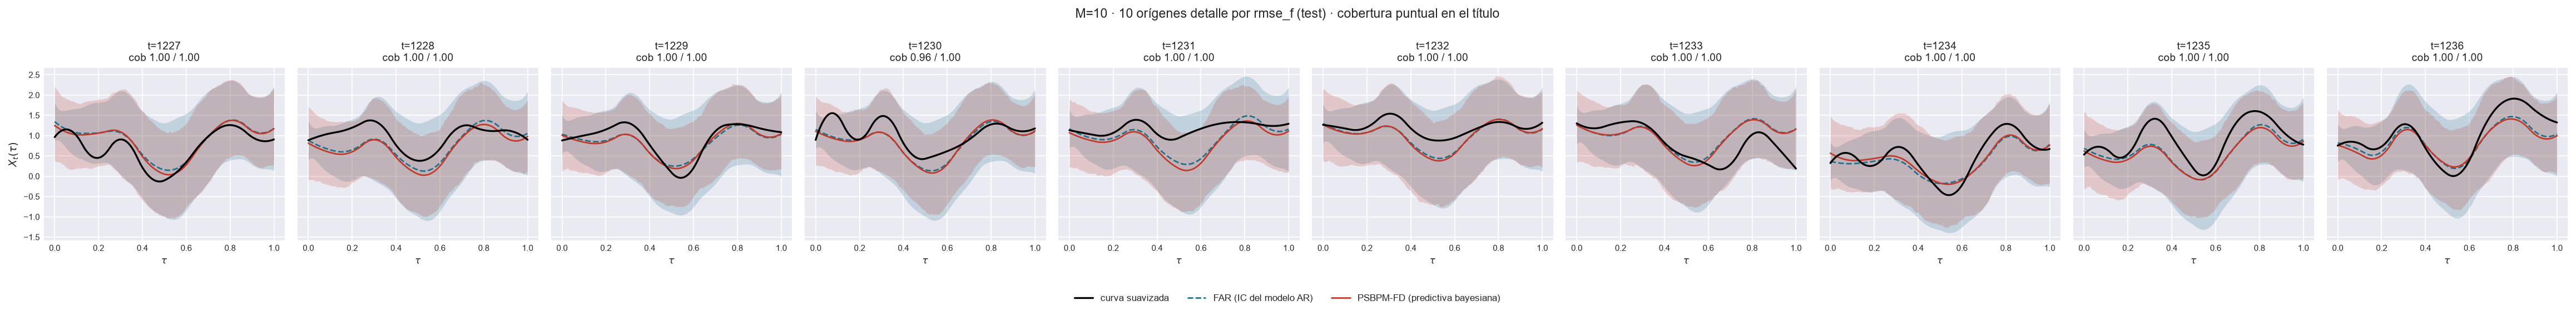
\includegraphics[width=\textwidth,height=0.75\textheight,keepaspectratio]{IMG/aneD_00/aneD_00_79_ic_contraste_detalle_103.png}
\caption{Precio SA1 (AEMO). Bandas equi-colas y del FAR en la ventana de detalle ($M = 10$).}
\label{fig:aneD_79_ic_contraste_detalle_103}
\end{figure}

\begin{figure}[H]
\centering
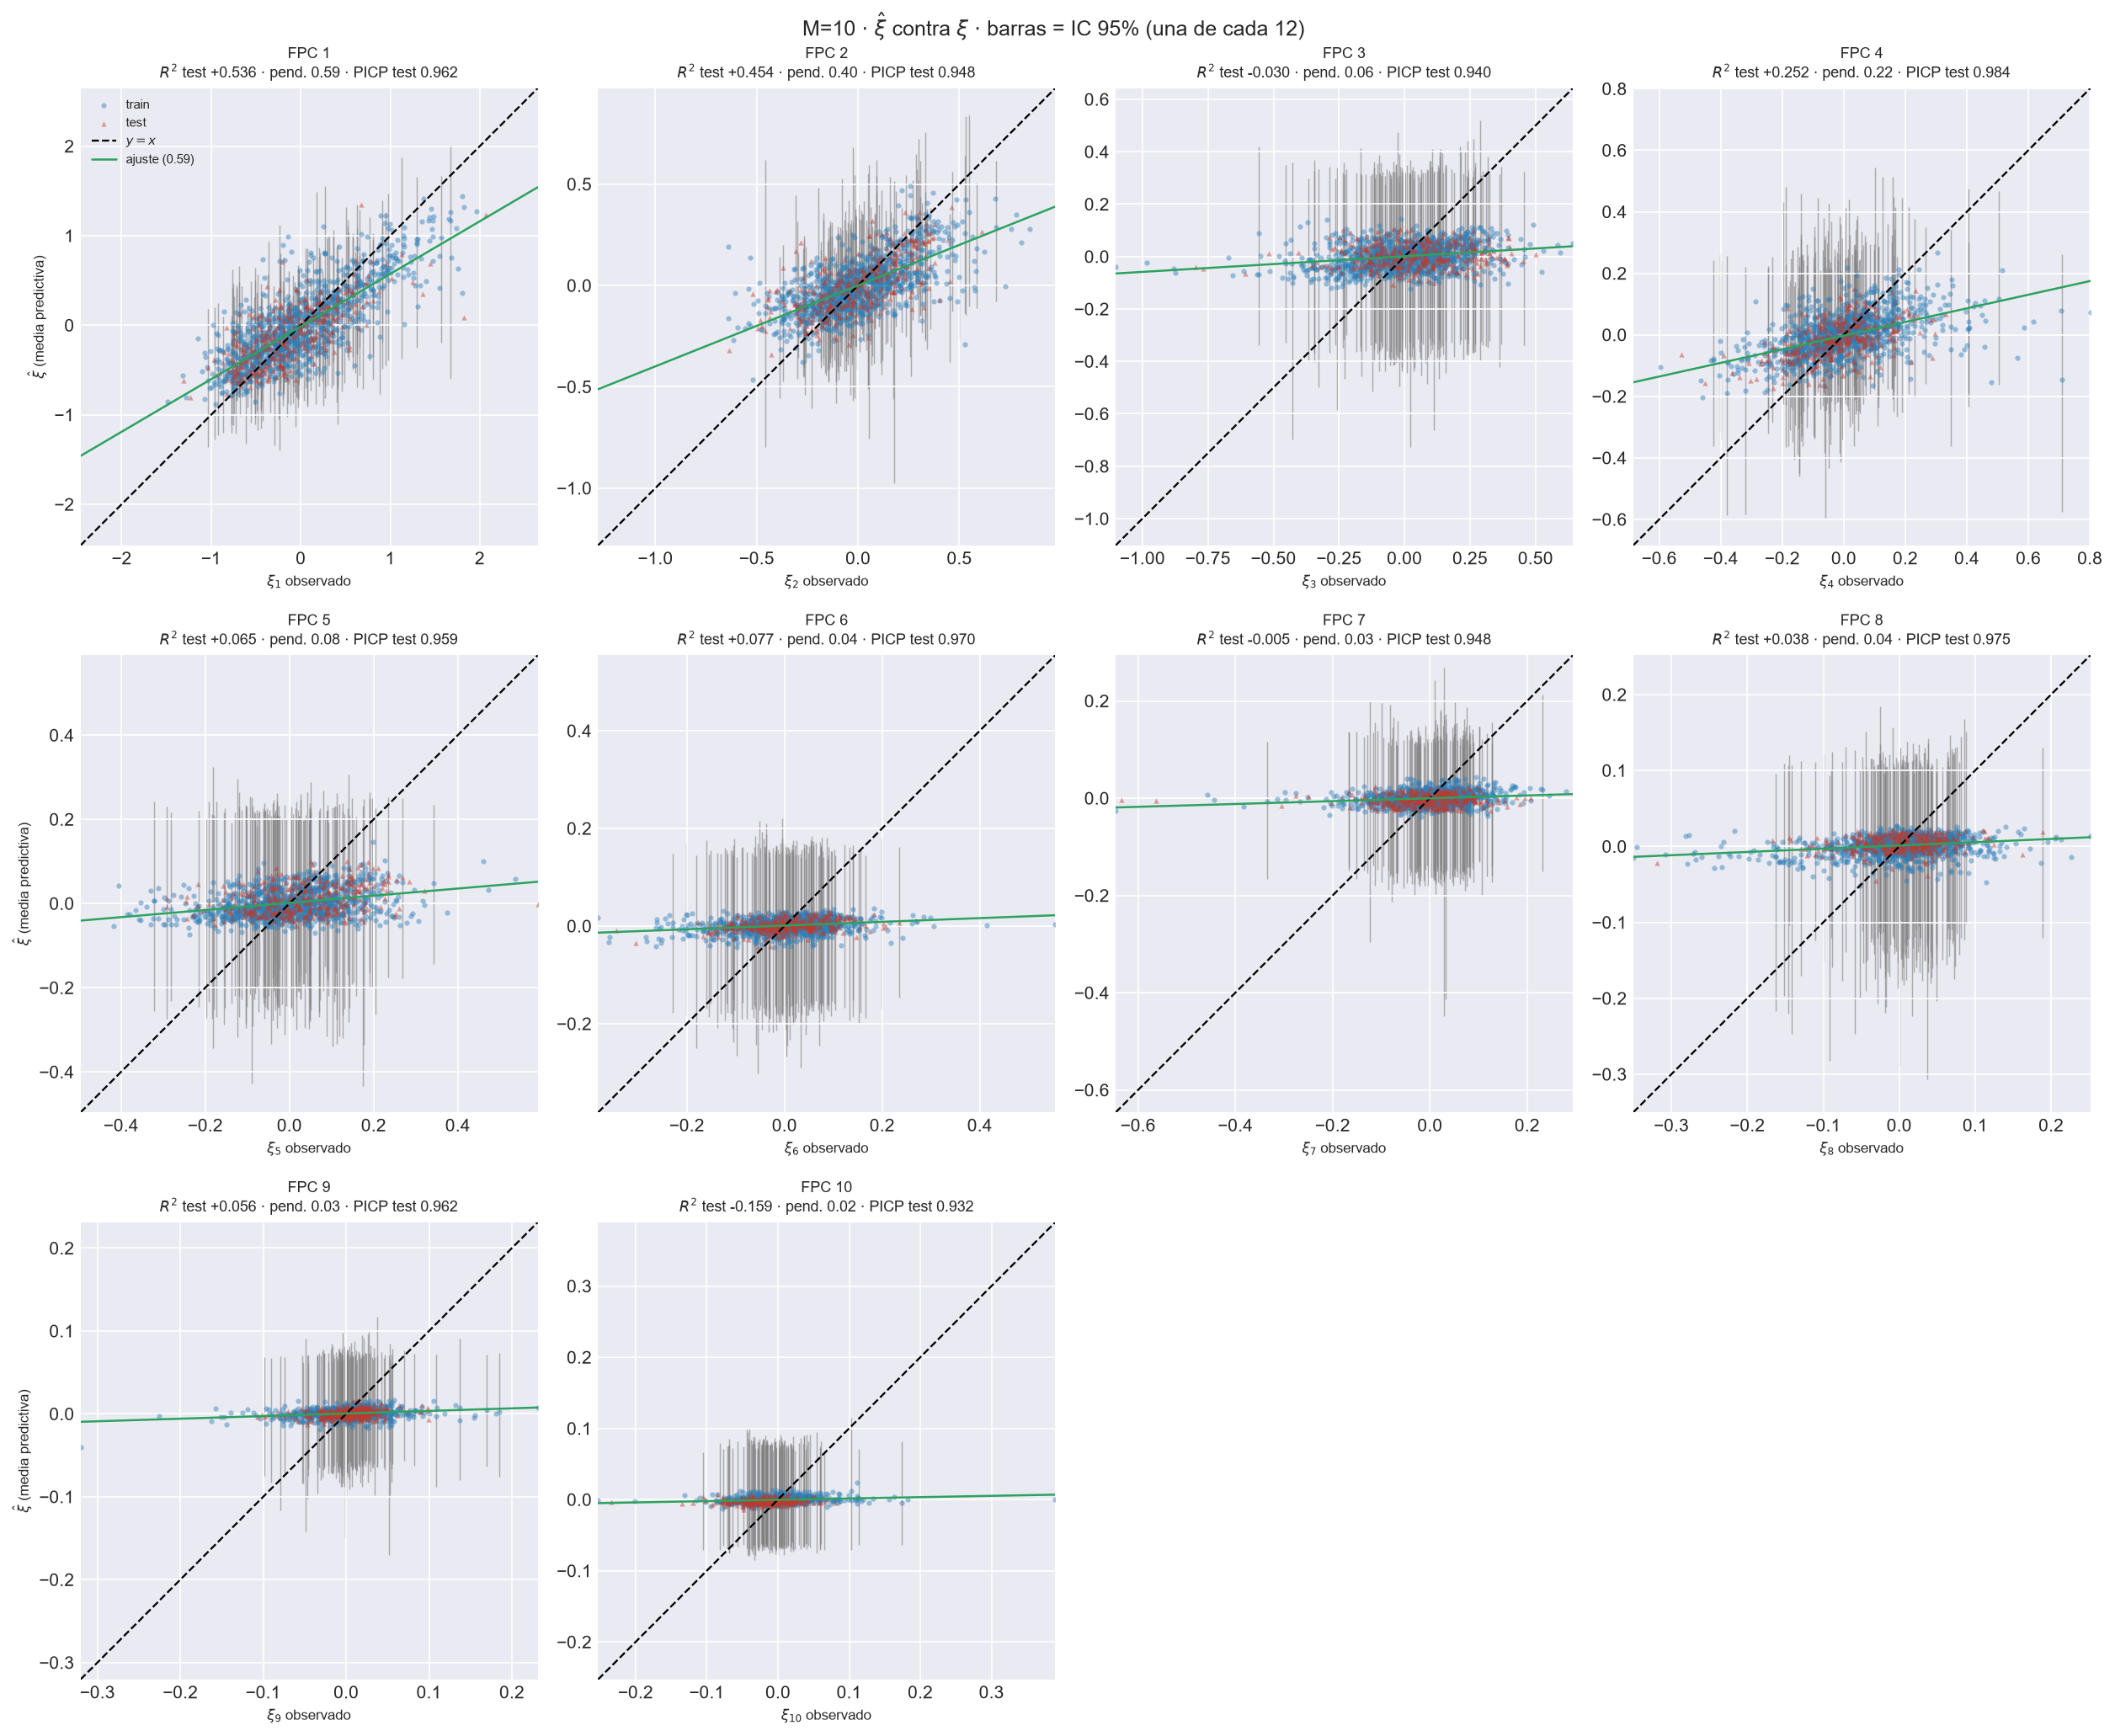
\includegraphics[width=\textwidth,height=0.75\textheight,keepaspectratio]{IMG/aneD_00/aneD_00_94_scores_dispersion_vs_real_103.png}
\caption{Precio SA1 (AEMO). Dispersión estimada de cada score frente a la observada ($M = 10$).}
\label{fig:aneD_94_scores_dispersion_vs_real_103}
\end{figure}

\subsection{PM2.5 Parque O'Higgins}
\label{aneD_00_05_104}

\begin{figure}[H]
\centering
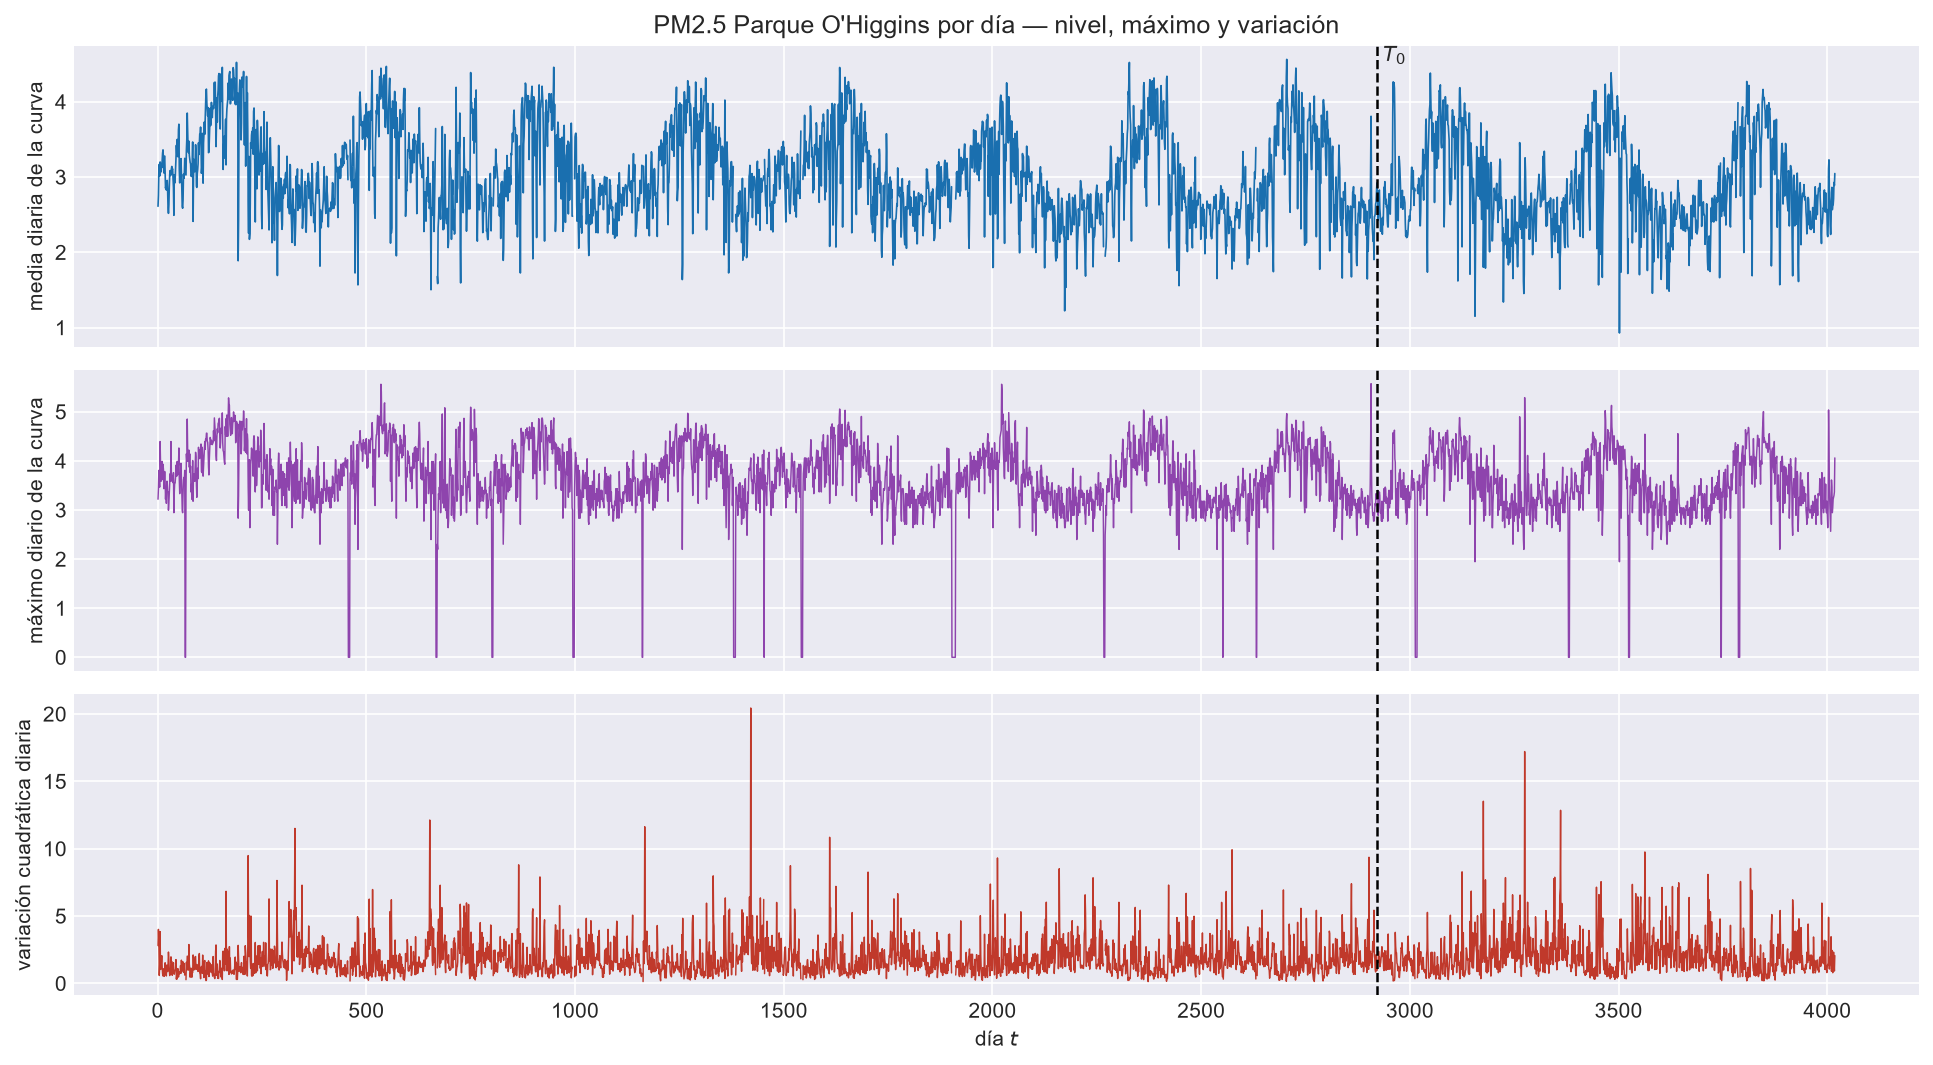
\includegraphics[width=\textwidth,height=0.75\textheight,keepaspectratio]{IMG/aneD_00/aneD_00_04_serie_diaria_104.png}
\caption{PM2.5 Parque O'Higgins. Serie diaria.}
\label{fig:aneD_04_serie_diaria_104}
\end{figure}

\begin{figure}[H]
\centering
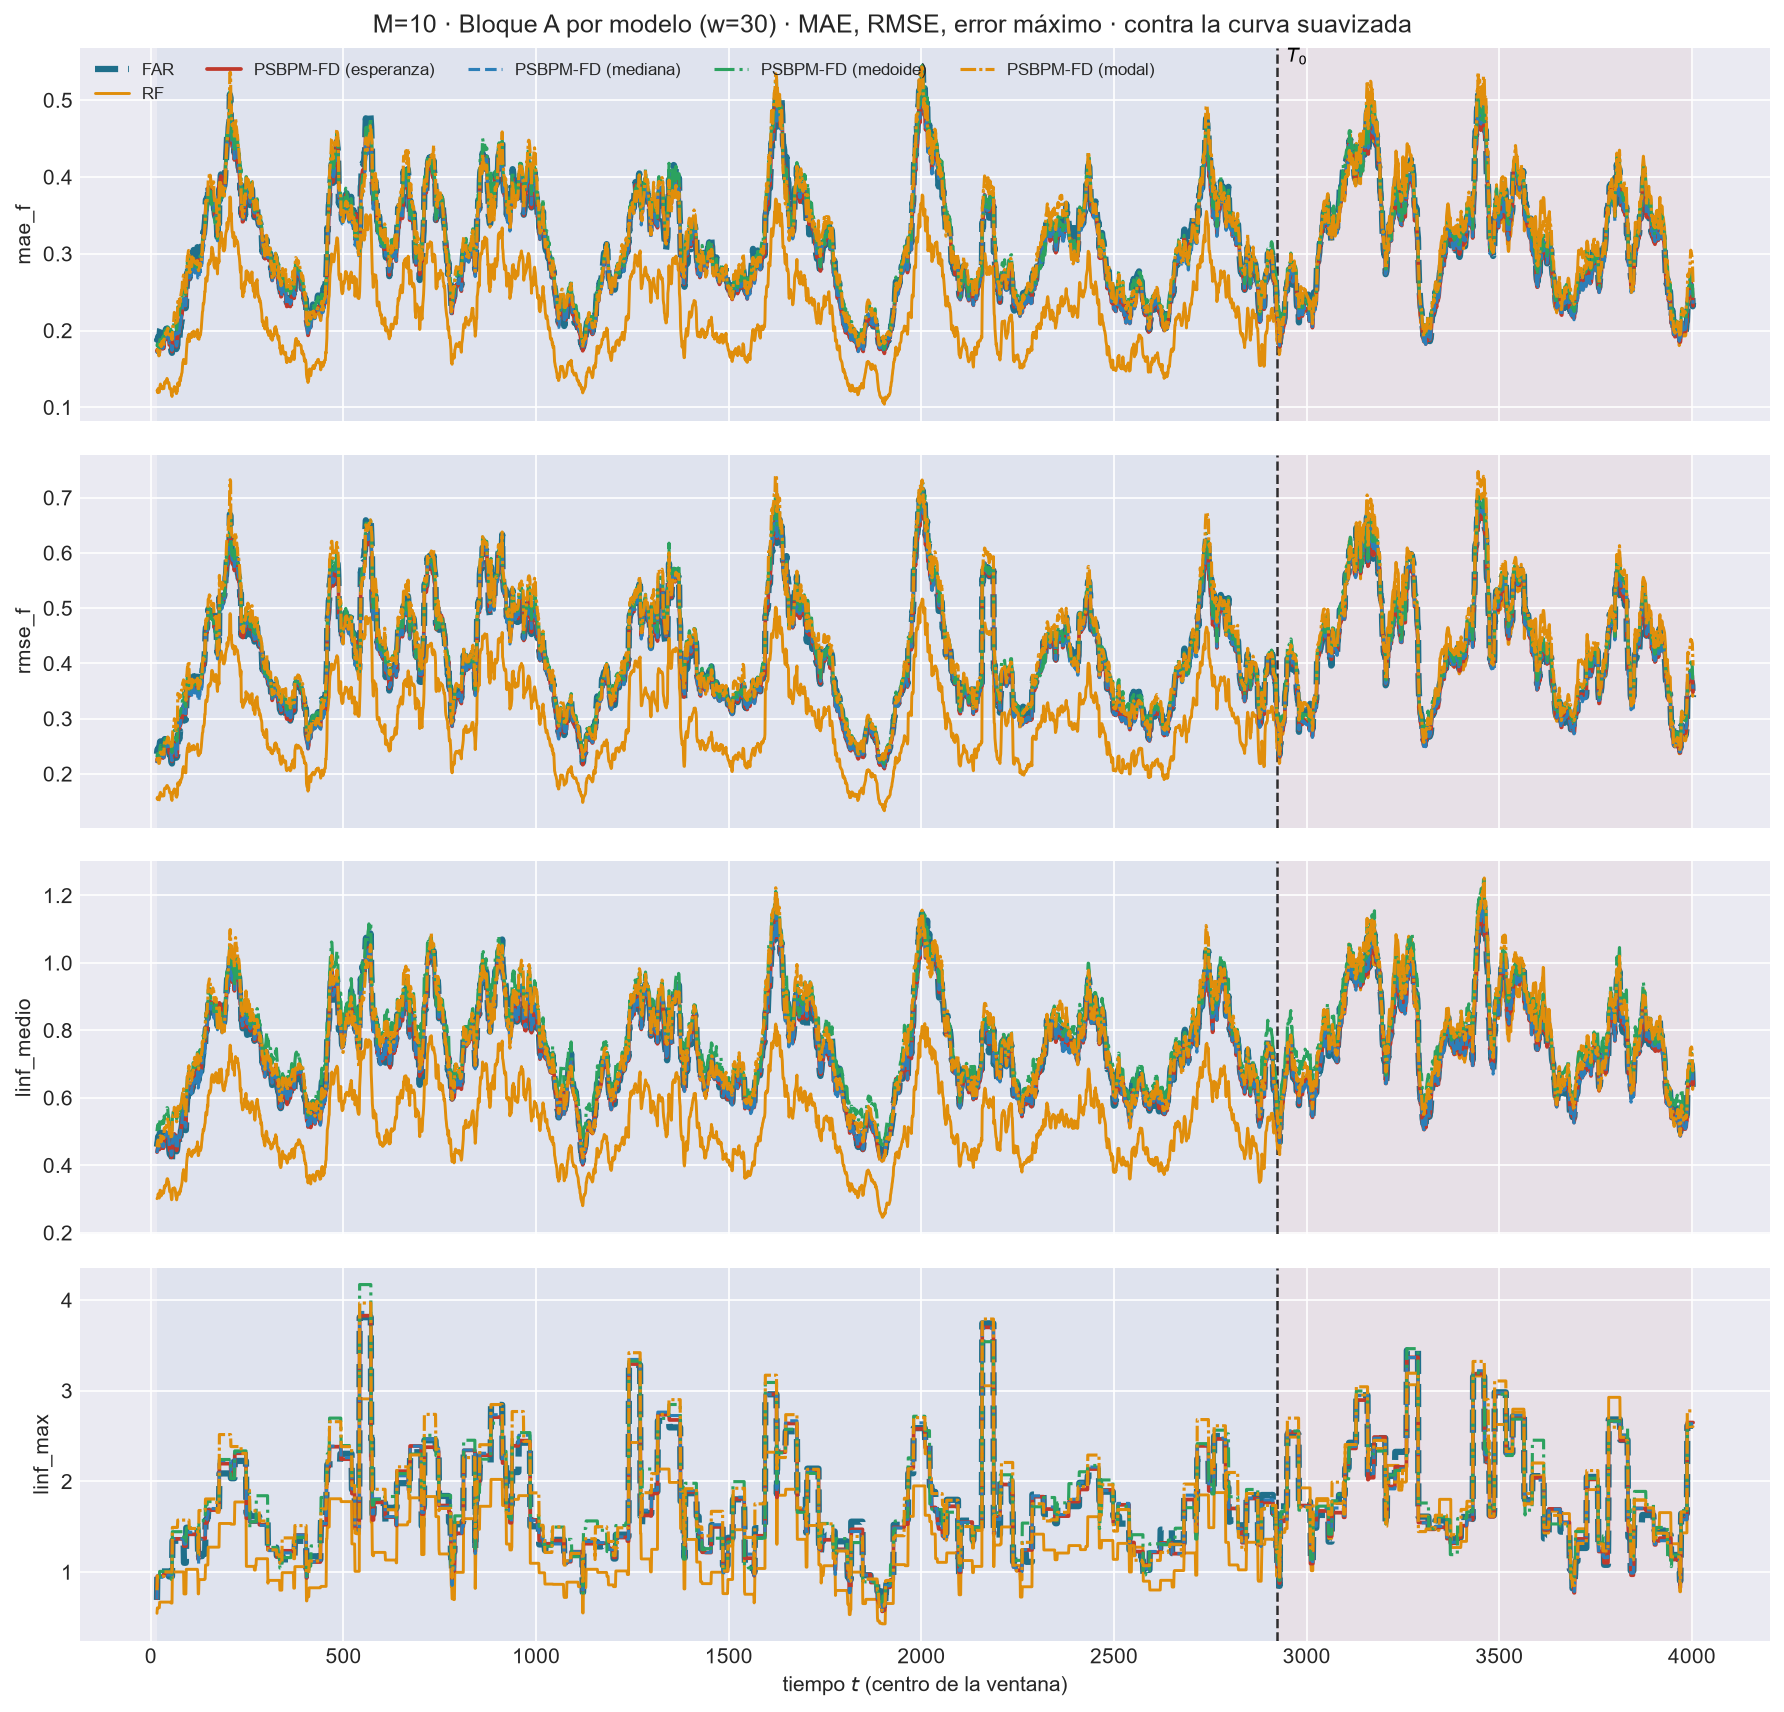
\includegraphics[width=\textwidth,height=0.75\textheight,keepaspectratio]{IMG/aneD_00/aneD_00_78_ventana_bloqueA_modelos_w30_104.png}
\caption{PM2.5 Parque O'Higgins. MAE sobre la ventana móvil del bloque de prueba ($M = 10$, $w = 30$).}
\label{fig:aneD_78_ventana_bloqueA_modelos_w30_104}
\end{figure}

\begin{figure}[H]
\centering
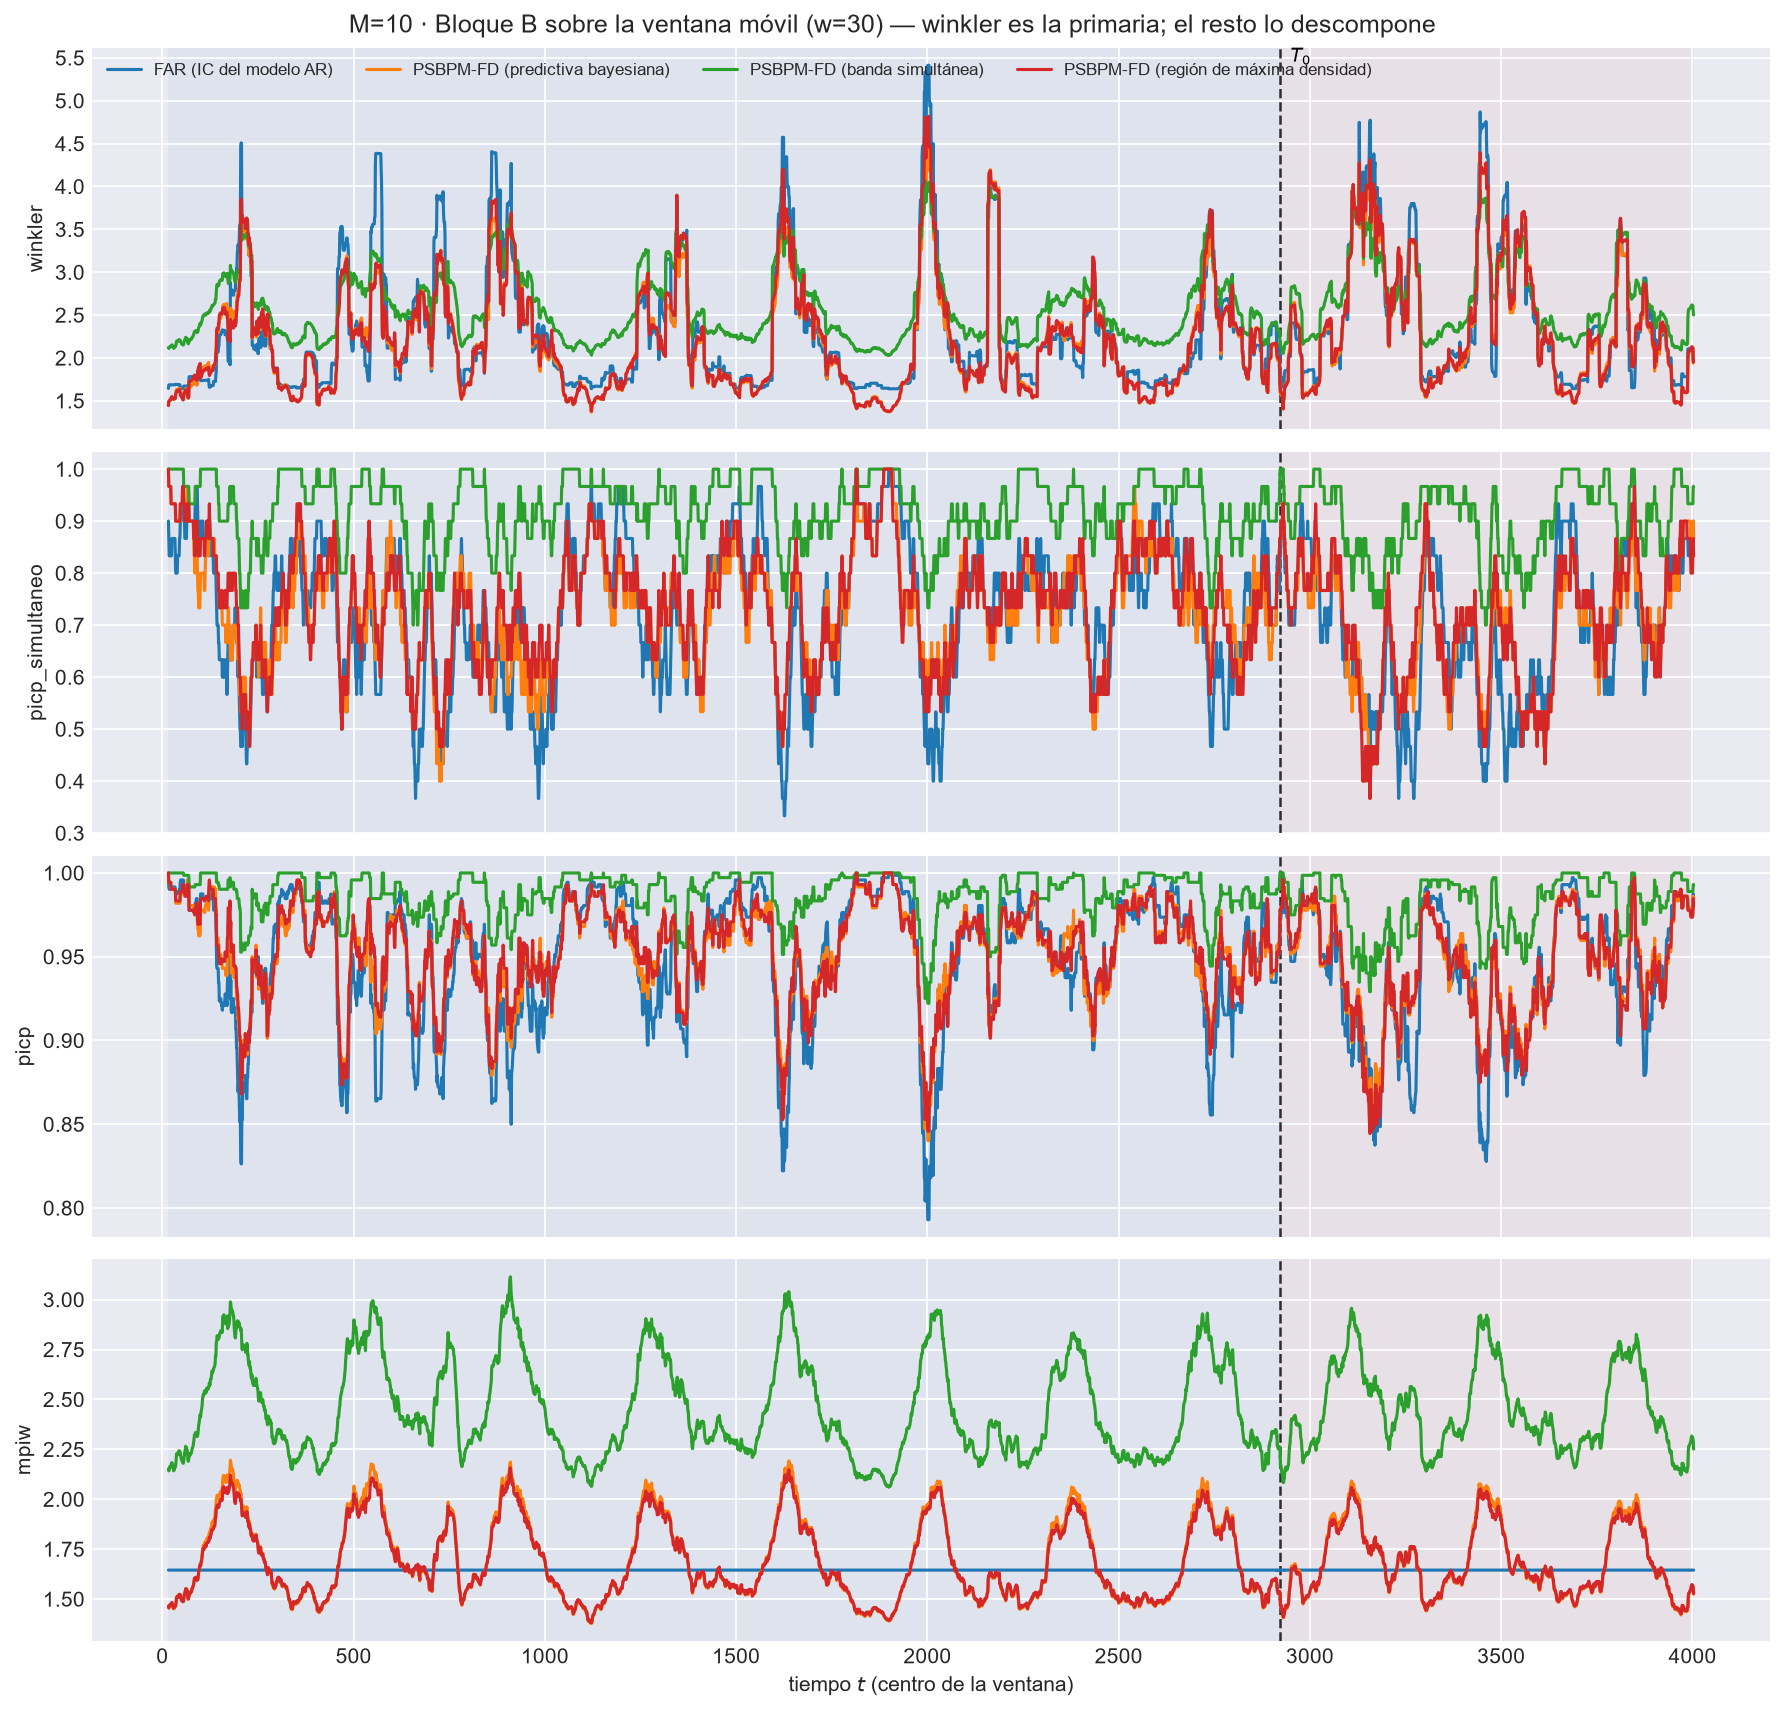
\includegraphics[width=\textwidth,height=0.75\textheight,keepaspectratio]{IMG/aneD_00/aneD_00_81_ventana_bloqueB_w30_104.png}
\caption{PM2.5 Parque O'Higgins. Winkler sobre la ventana móvil del bloque de prueba ($M = 10$, $w = 30$).}
\label{fig:aneD_81_ventana_bloqueB_w30_104}
\end{figure}

\begin{figure}[H]
\centering
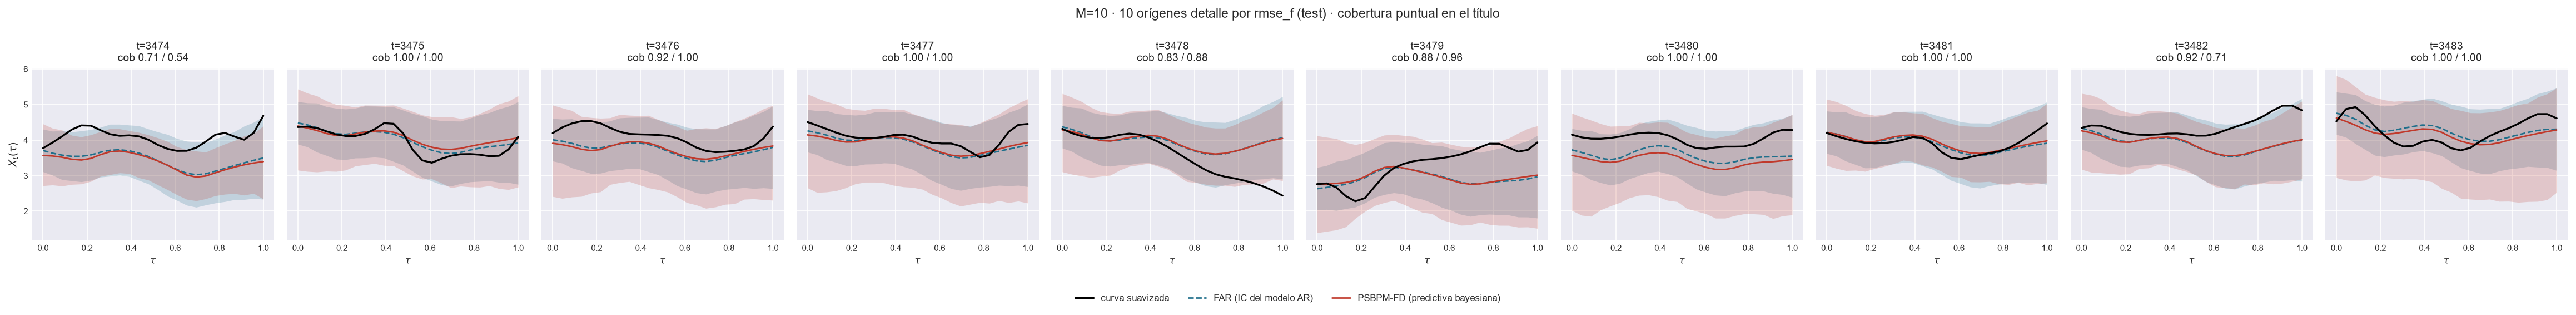
\includegraphics[width=\textwidth,height=0.75\textheight,keepaspectratio]{IMG/aneD_00/aneD_00_79_ic_contraste_detalle_104.png}
\caption{PM2.5 Parque O'Higgins. Bandas equi-colas y del FAR en la ventana de detalle ($M = 10$).}
\label{fig:aneD_79_ic_contraste_detalle_104}
\end{figure}

\begin{figure}[H]
\centering
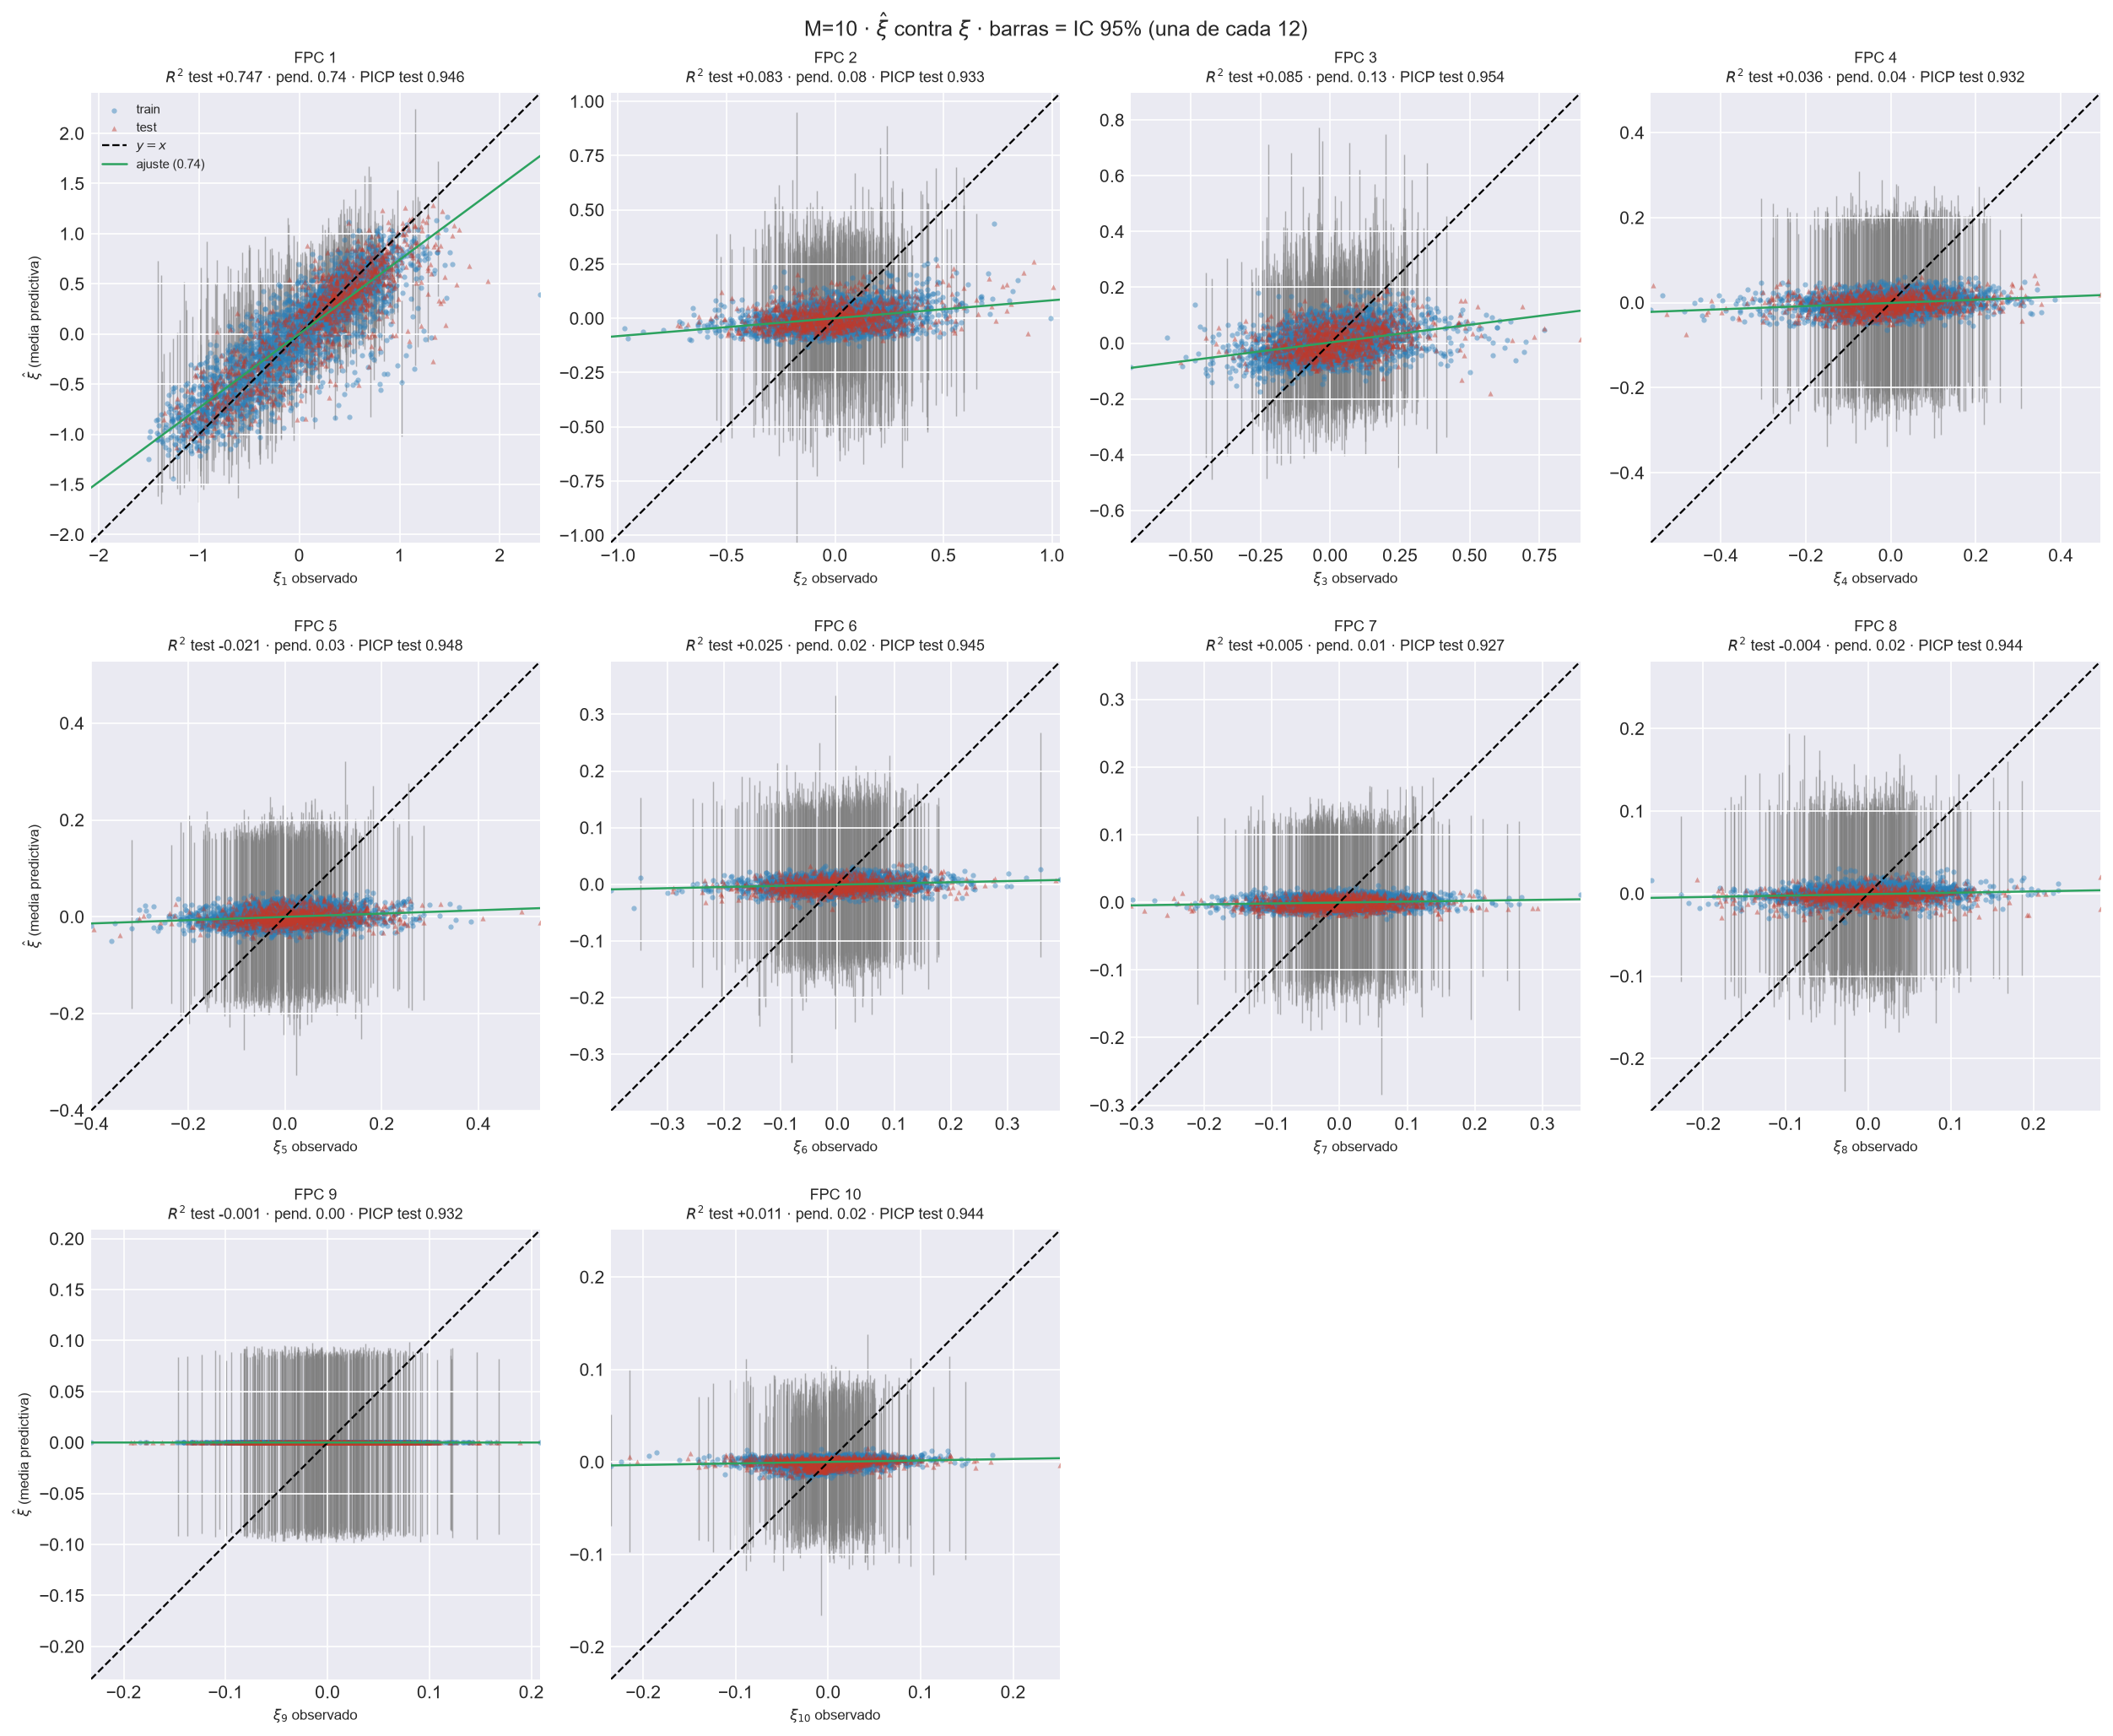
\includegraphics[width=\textwidth,height=0.75\textheight,keepaspectratio]{IMG/aneD_00/aneD_00_94_scores_dispersion_vs_real_104.png}
\caption{PM2.5 Parque O'Higgins. Dispersión estimada de cada score frente a la observada ($M = 10$).}
\label{fig:aneD_94_scores_dispersion_vs_real_104}
\end{figure}

\subsection{PM2.5 Beijing}
\label{aneD_00_05_105}

\begin{figure}[H]
\centering
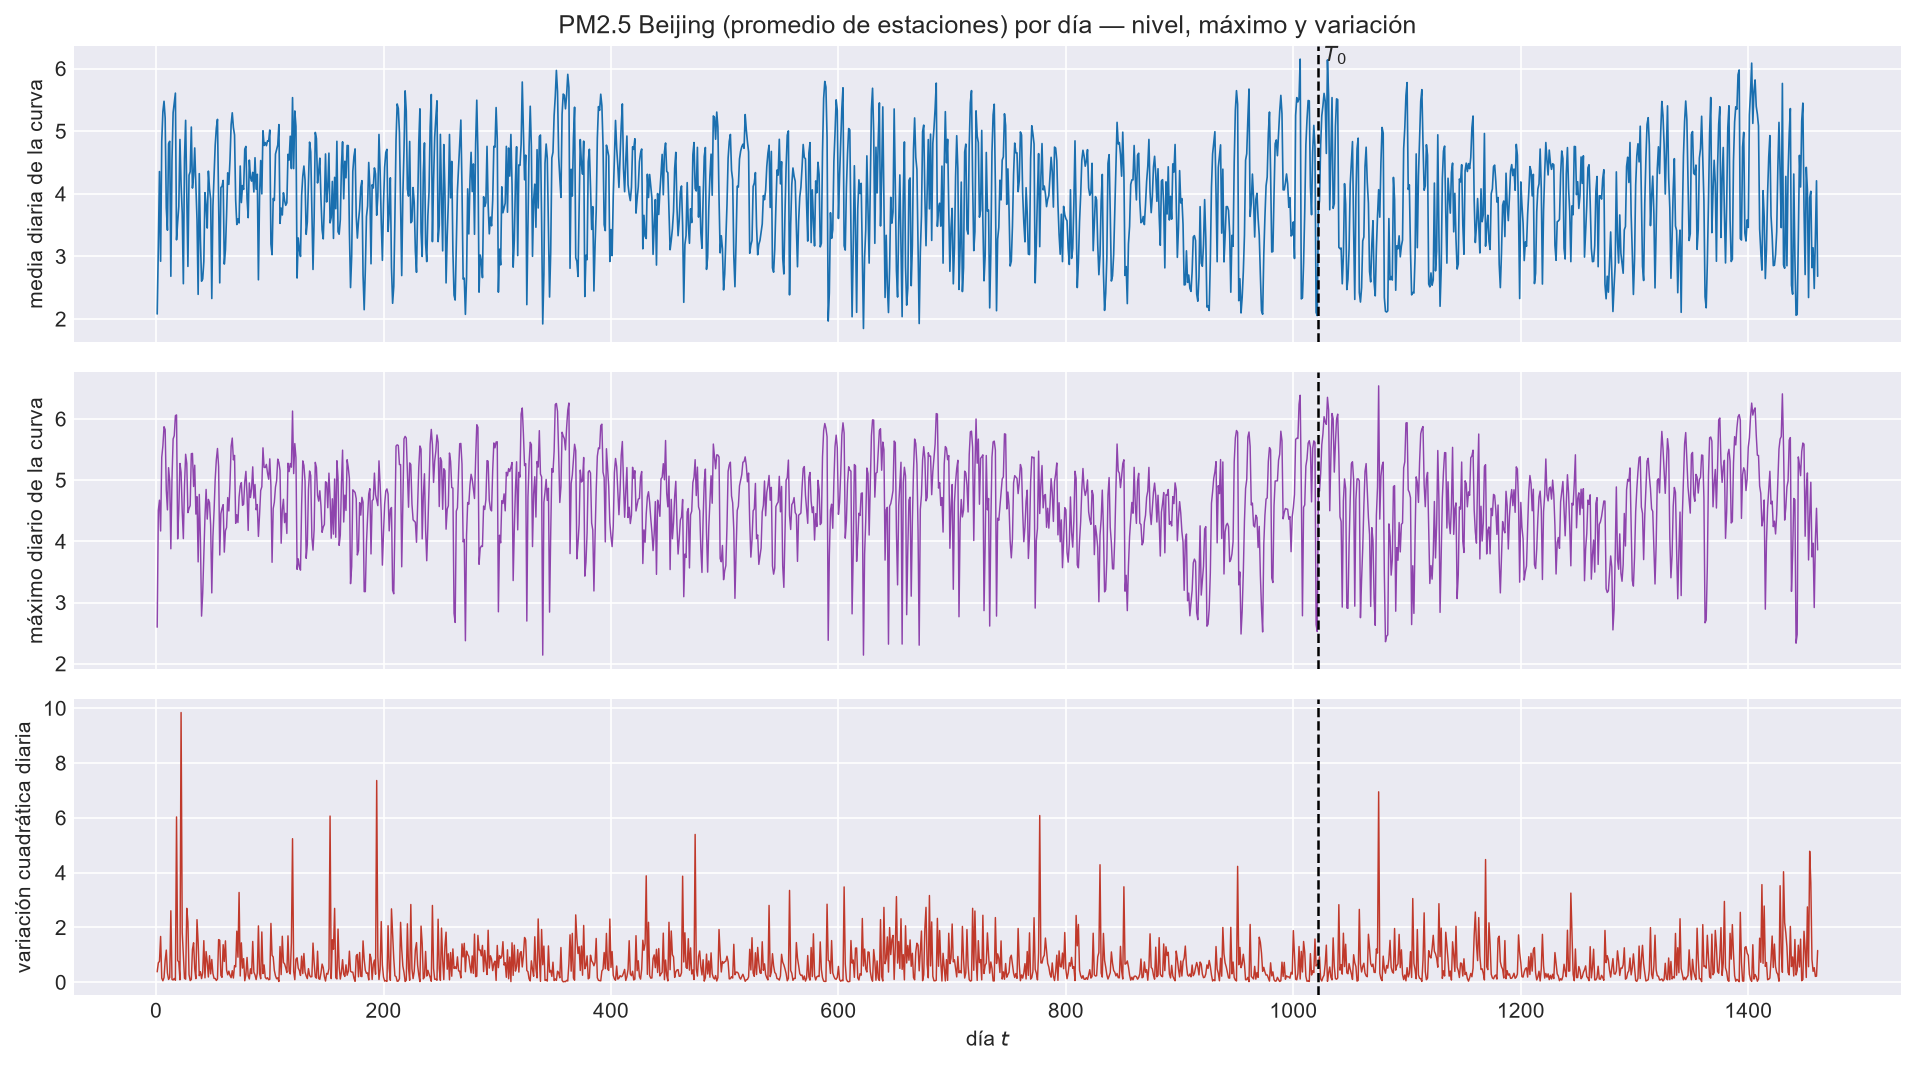
\includegraphics[width=\textwidth,height=0.75\textheight,keepaspectratio]{IMG/aneD_00/aneD_00_04_serie_diaria_105.png}
\caption{PM2.5 Beijing. Serie diaria.}
\label{fig:aneD_04_serie_diaria_105}
\end{figure}

\begin{figure}[H]
\centering
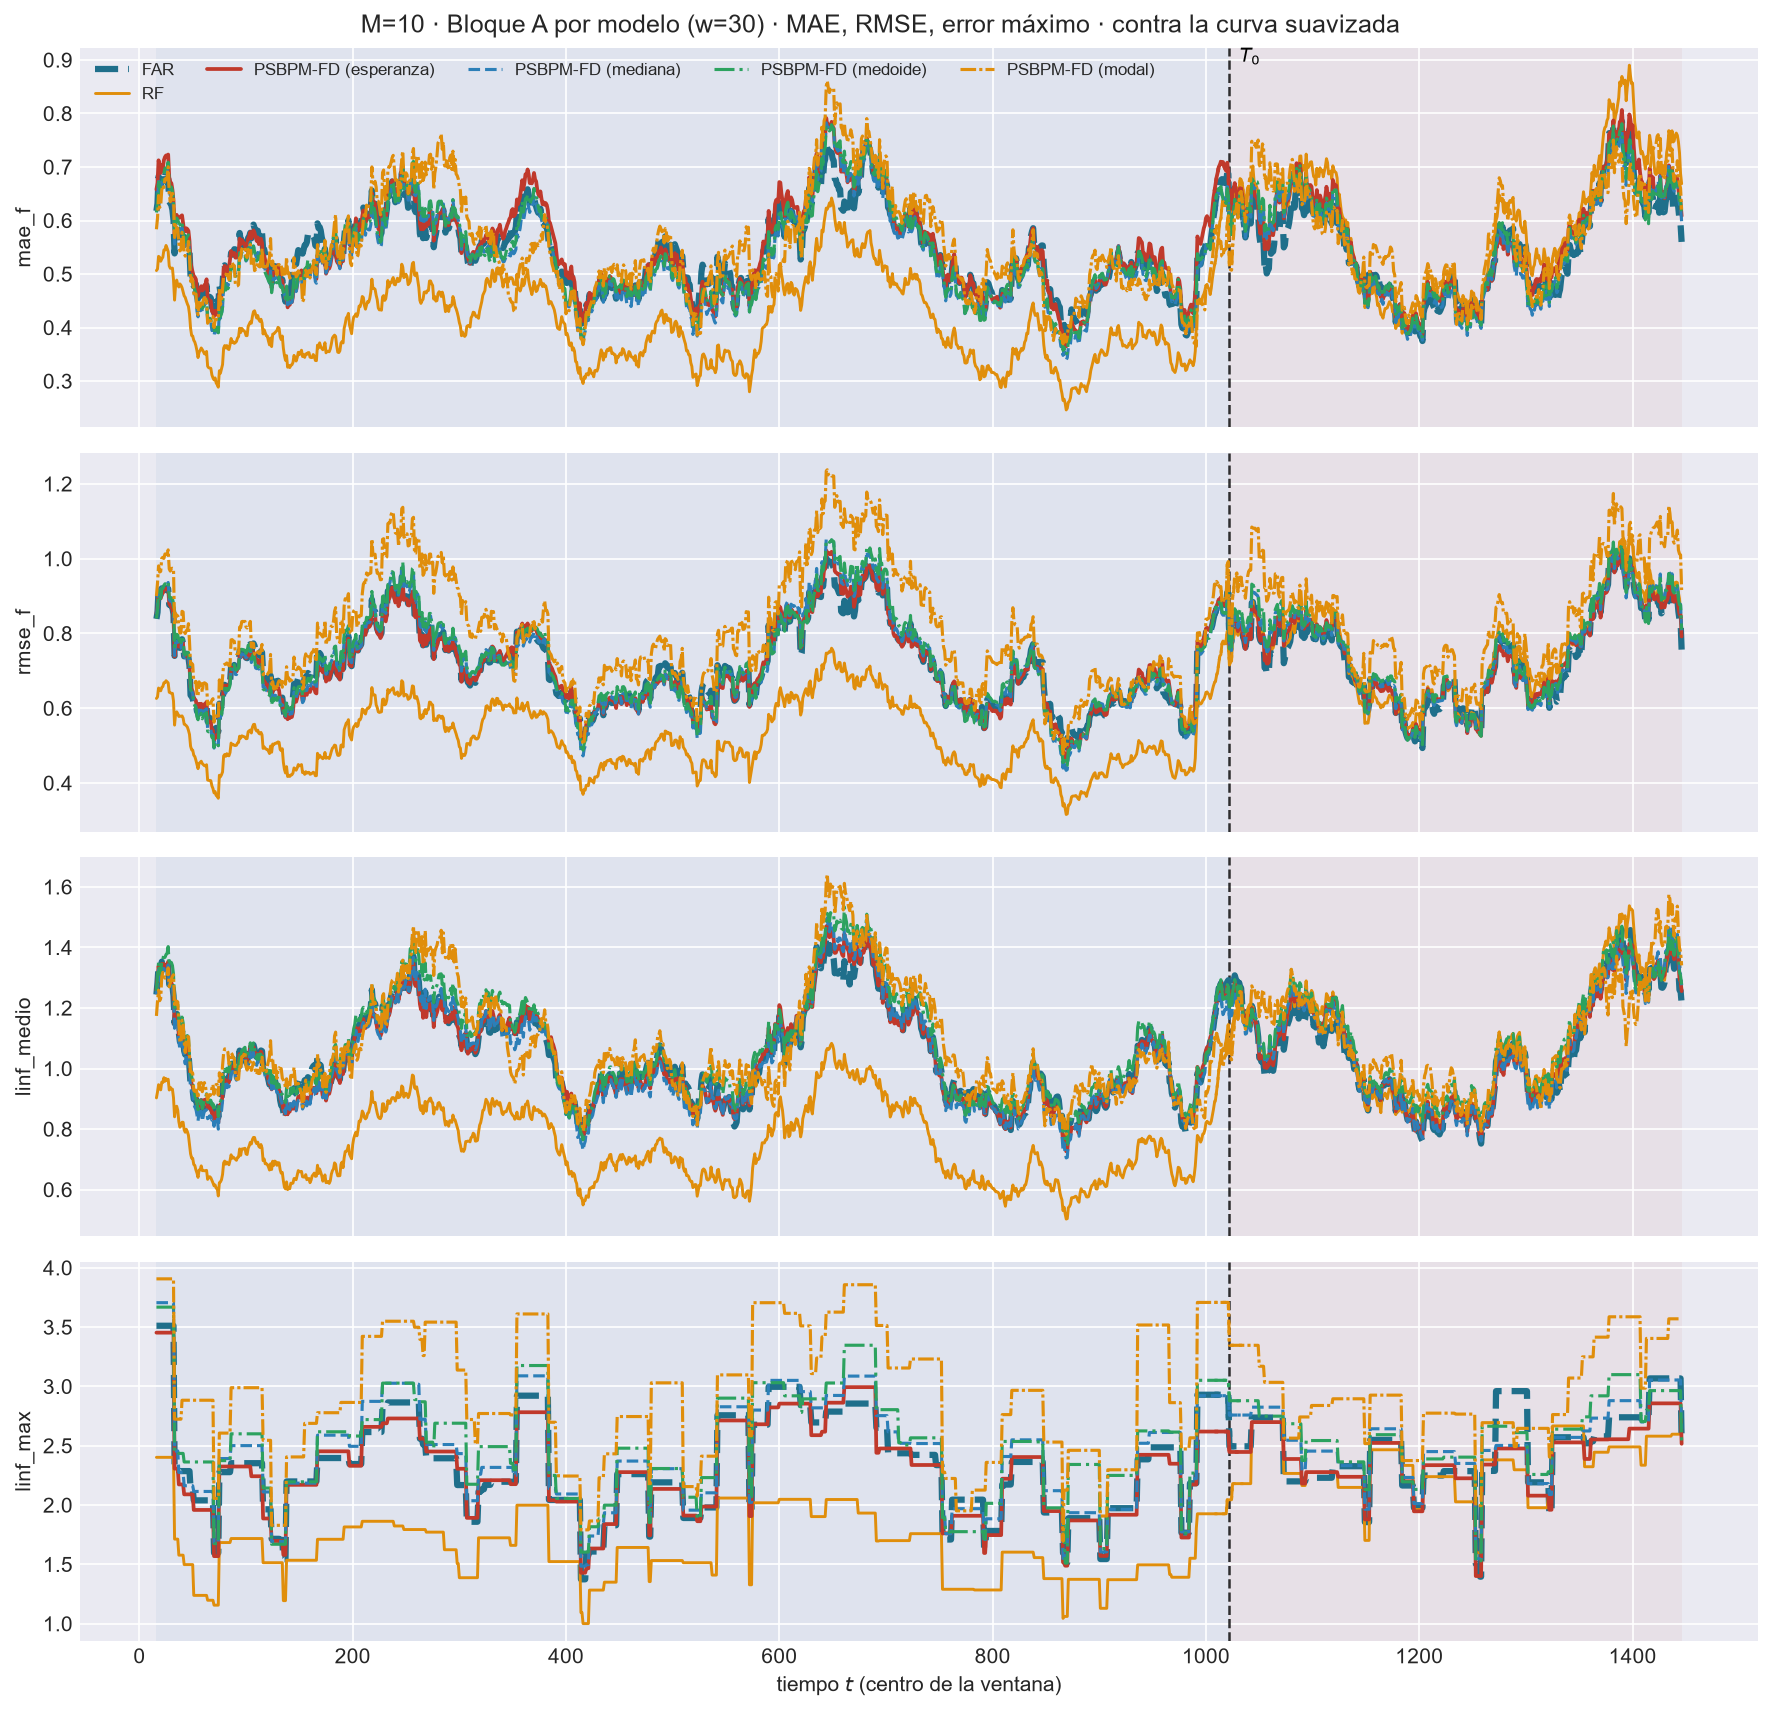
\includegraphics[width=\textwidth,height=0.75\textheight,keepaspectratio]{IMG/aneD_00/aneD_00_78_ventana_bloqueA_modelos_w30_105.png}
\caption{PM2.5 Beijing. MAE sobre la ventana móvil del bloque de prueba ($M = 10$, $w = 30$).}
\label{fig:aneD_78_ventana_bloqueA_modelos_w30_105}
\end{figure}

\begin{figure}[H]
\centering
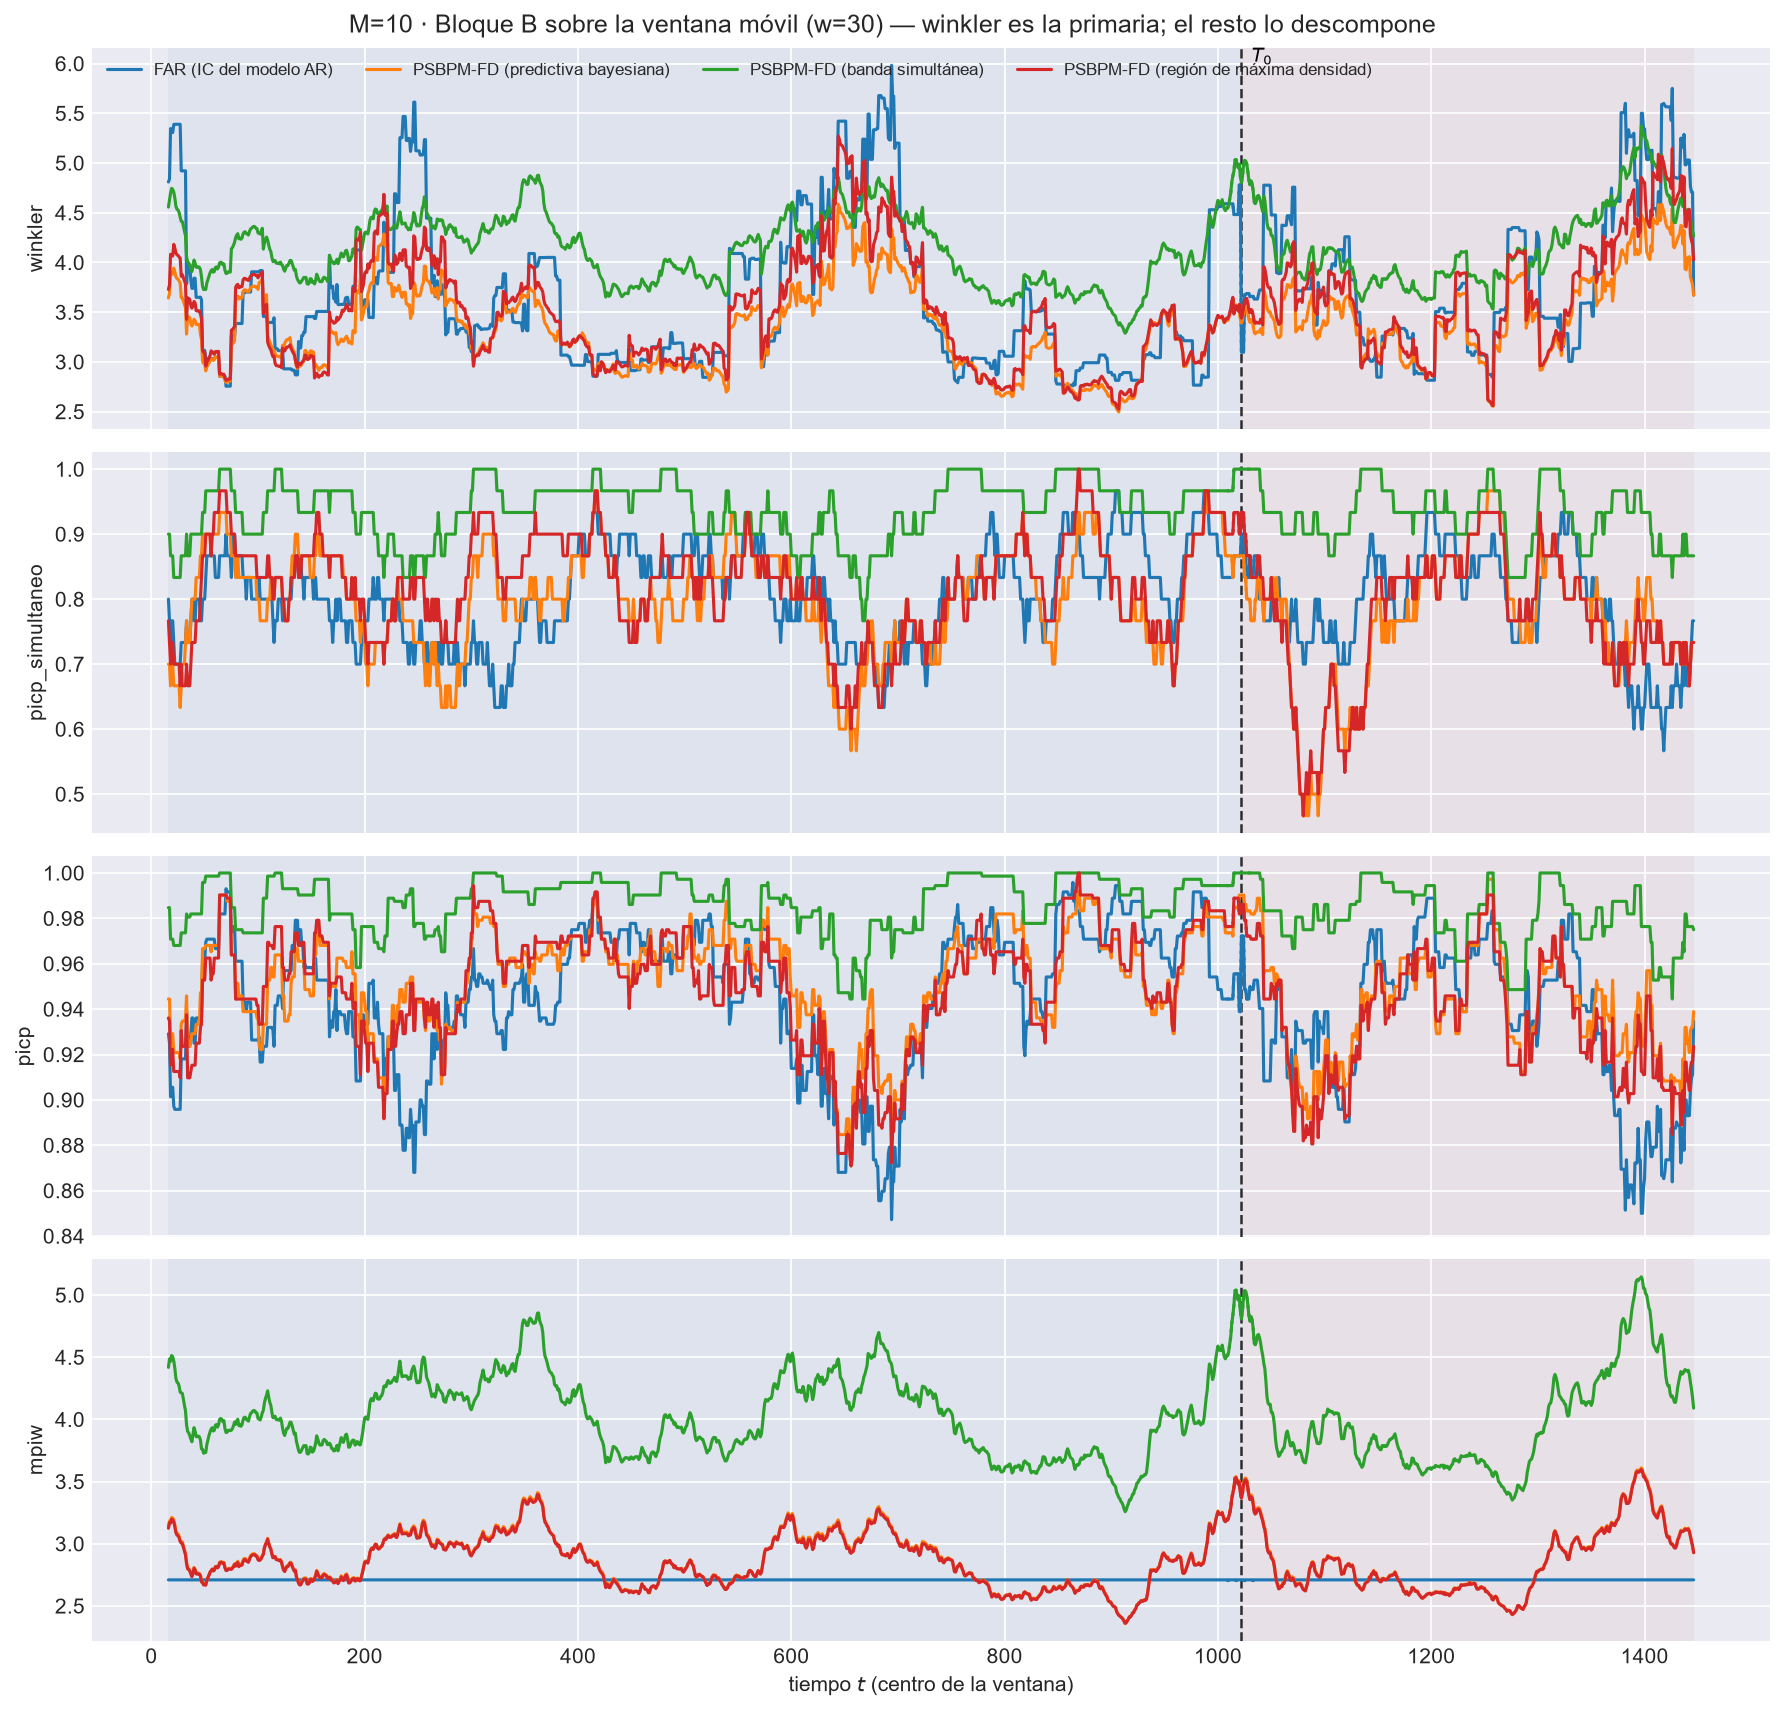
\includegraphics[width=\textwidth,height=0.75\textheight,keepaspectratio]{IMG/aneD_00/aneD_00_81_ventana_bloqueB_w30_105.png}
\caption{PM2.5 Beijing. Winkler sobre la ventana móvil del bloque de prueba ($M = 10$, $w = 30$).}
\label{fig:aneD_81_ventana_bloqueB_w30_105}
\end{figure}

\begin{figure}[H]
\centering
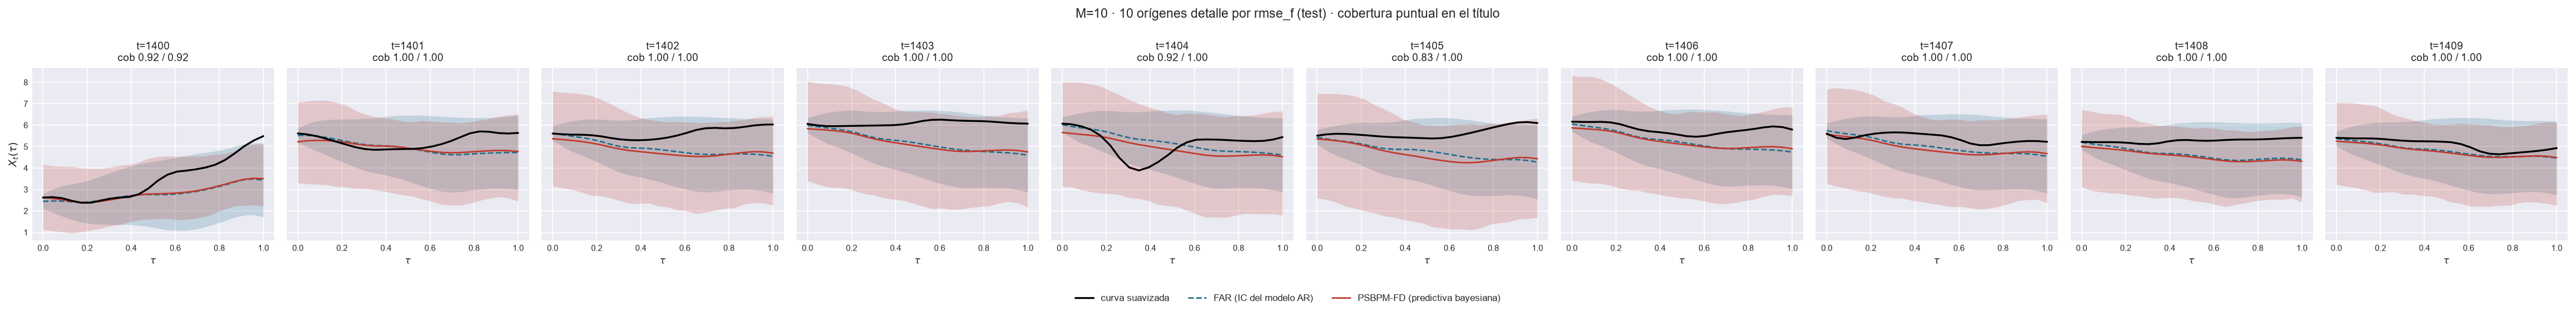
\includegraphics[width=\textwidth,height=0.75\textheight,keepaspectratio]{IMG/aneD_00/aneD_00_79_ic_contraste_detalle_105.png}
\caption{PM2.5 Beijing. Bandas equi-colas y del FAR en la ventana de detalle ($M = 10$).}
\label{fig:aneD_79_ic_contraste_detalle_105}
\end{figure}

\begin{figure}[H]
\centering
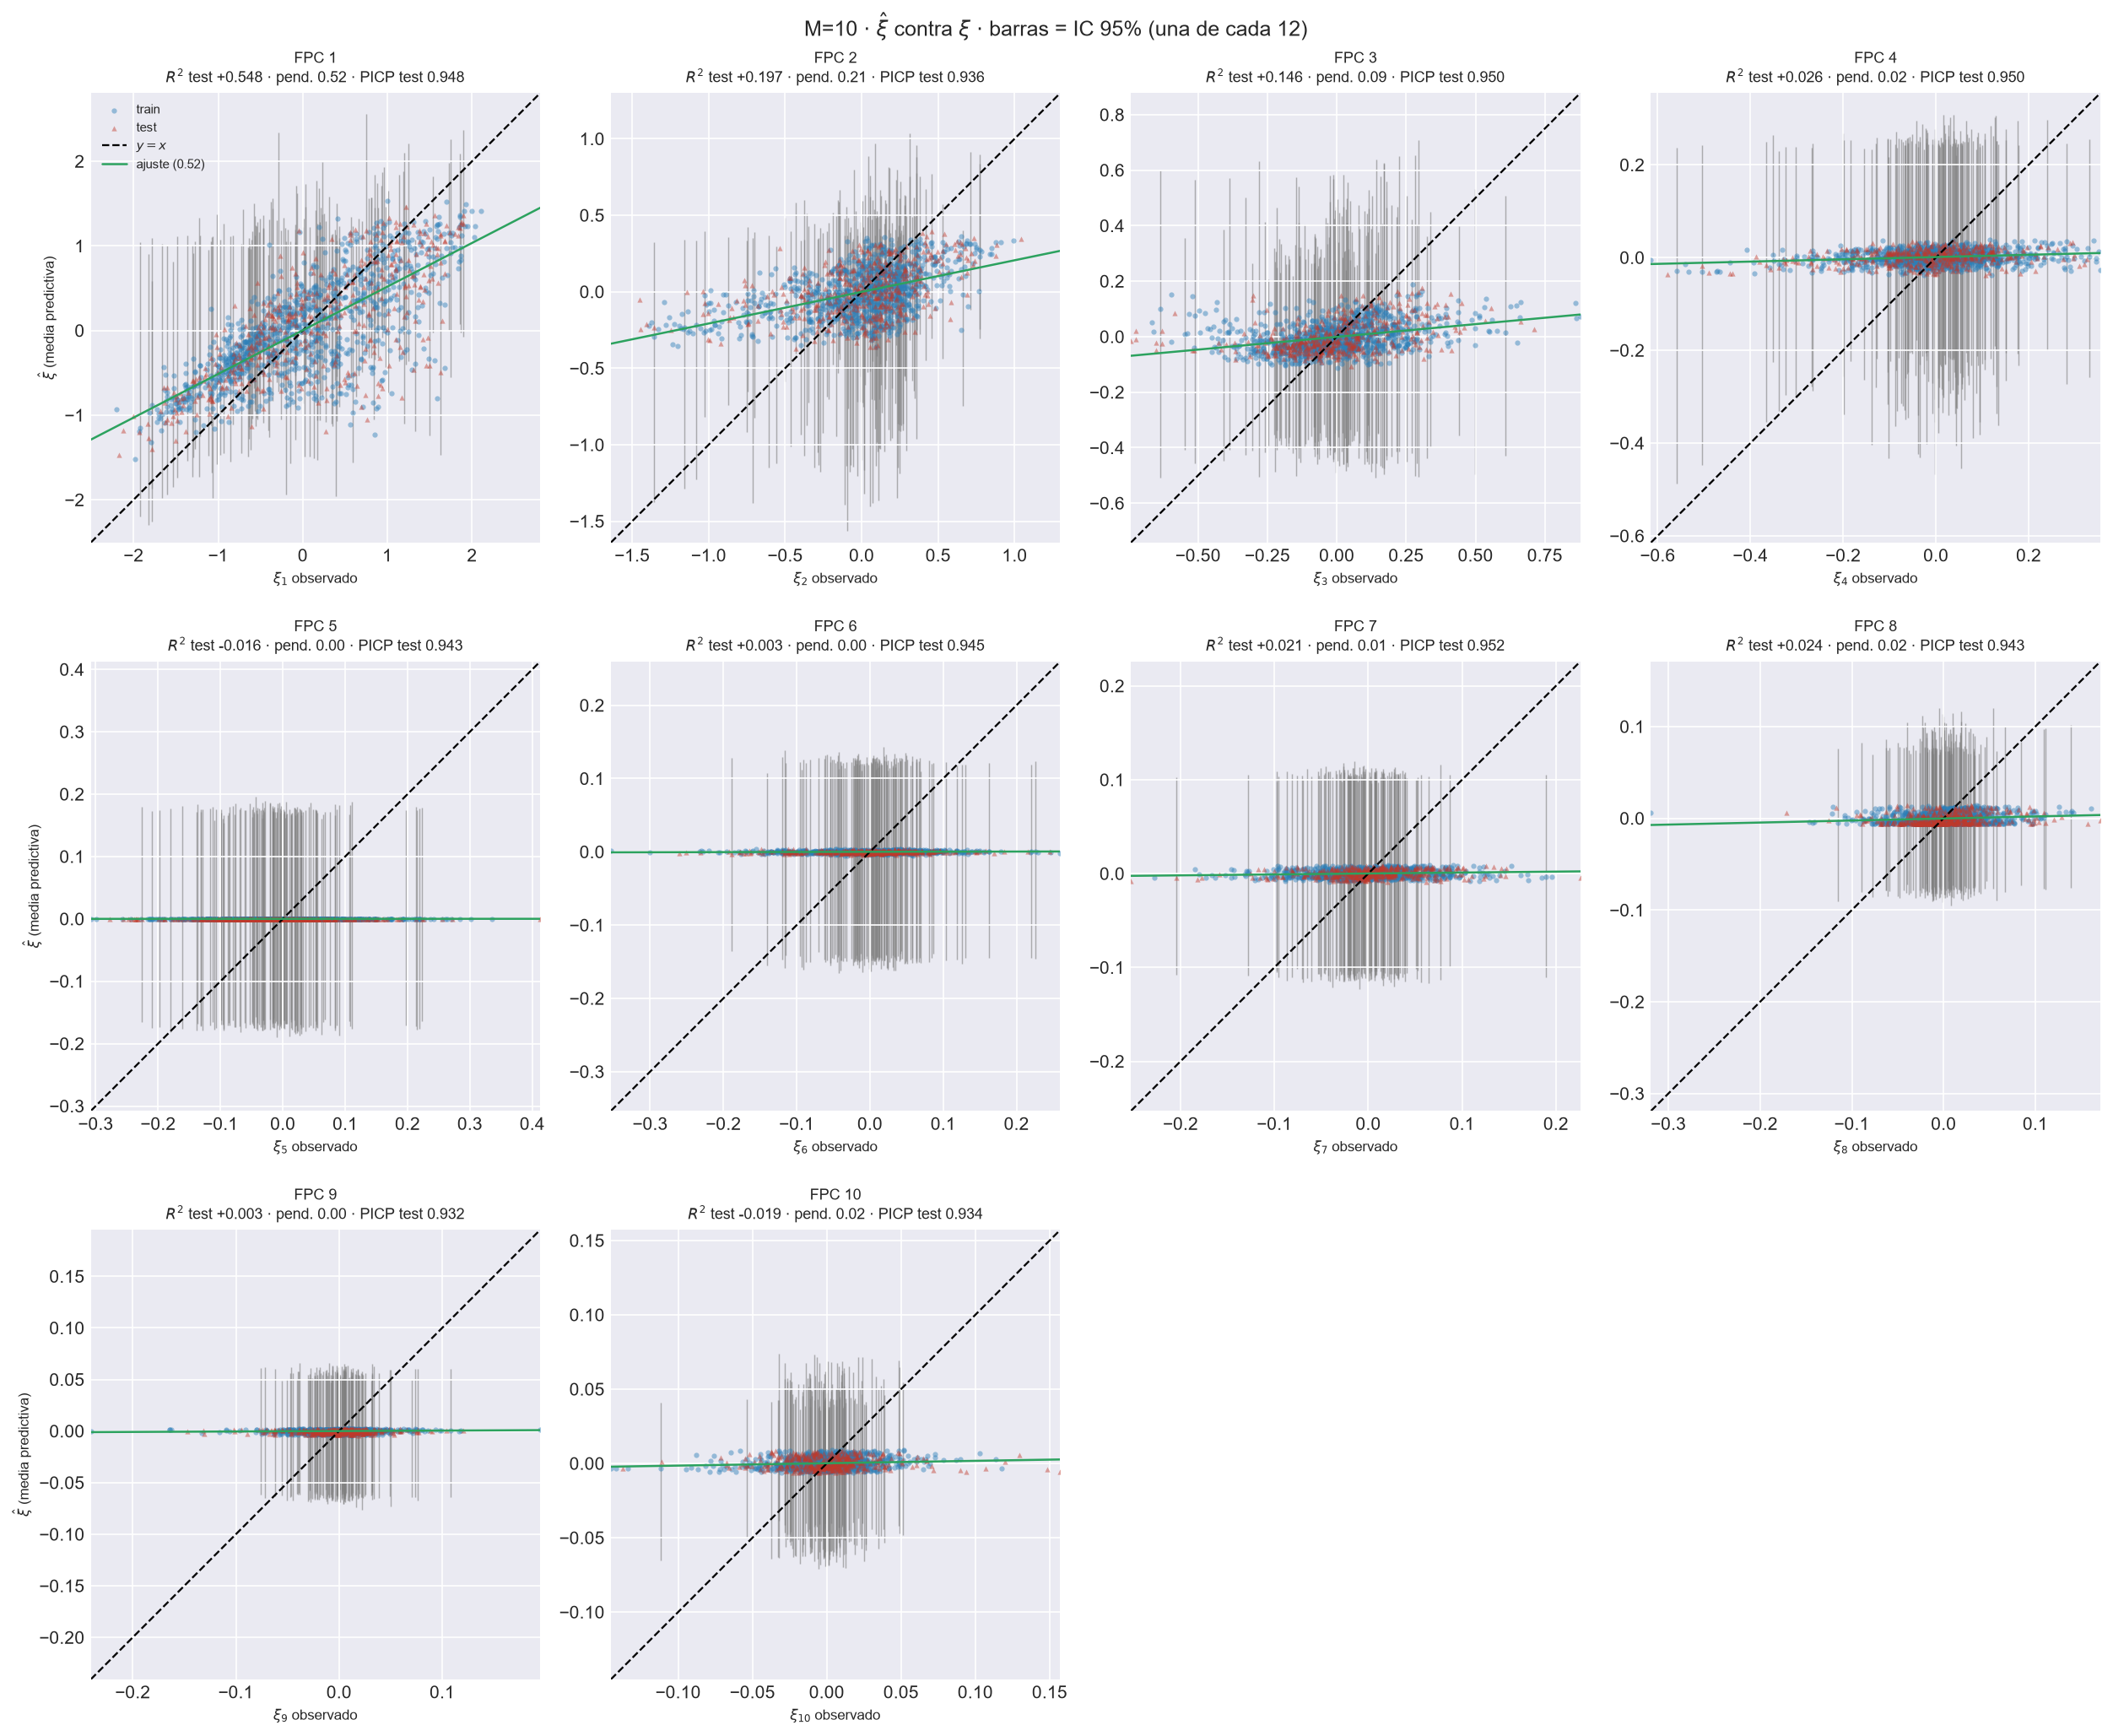
\includegraphics[width=\textwidth,height=0.75\textheight,keepaspectratio]{IMG/aneD_00/aneD_00_94_scores_dispersion_vs_real_105.png}
\caption{PM2.5 Beijing. Dispersión estimada de cada score frente a la observada ($M = 10$).}
\label{fig:aneD_94_scores_dispersion_vs_real_105}
\end{figure}

\subsection{Factor de planta eólico (SMARD)}
\label{aneD_00_05_106}

\begin{figure}[H]
\centering
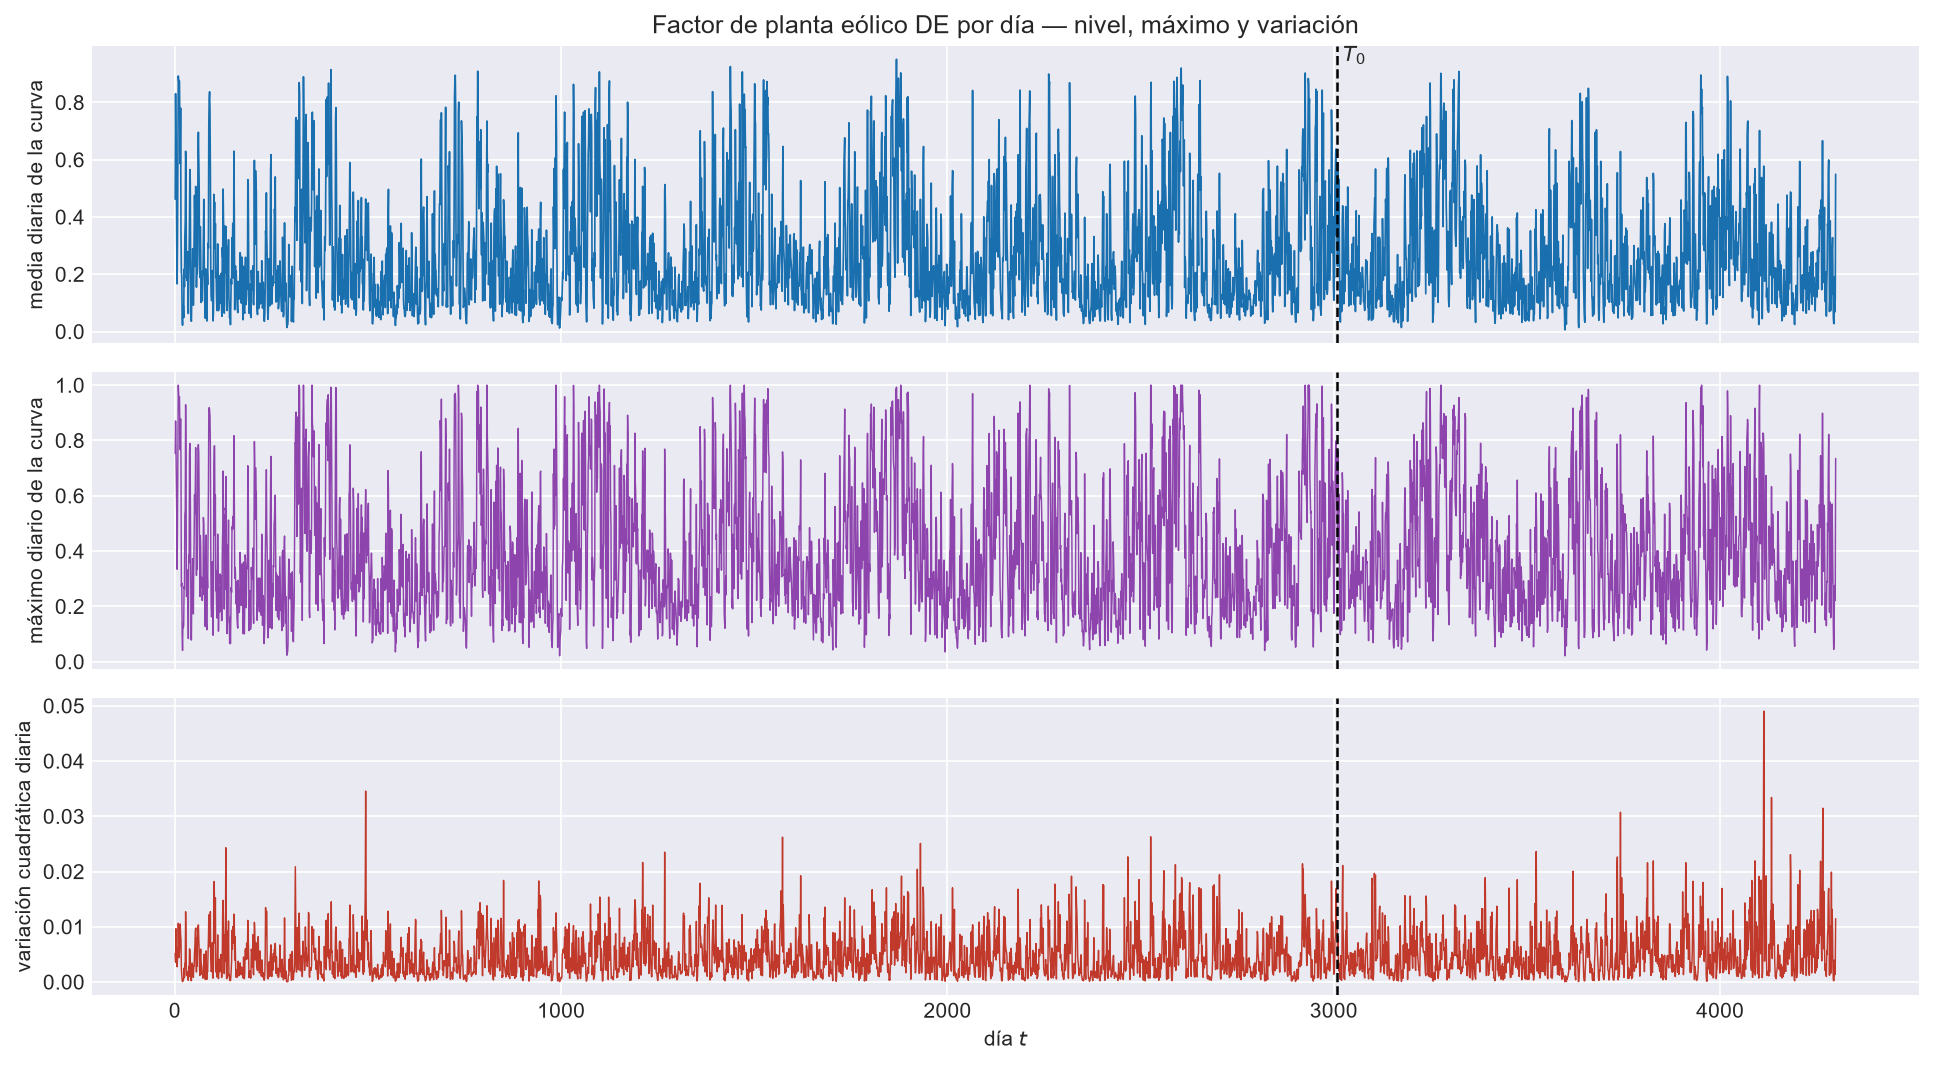
\includegraphics[width=\textwidth,height=0.75\textheight,keepaspectratio]{IMG/aneD_00/aneD_00_04_serie_diaria_106.png}
\caption{Factor de planta eólico (SMARD). Serie diaria.}
\label{fig:aneD_04_serie_diaria_106}
\end{figure}

\begin{figure}[H]
\centering
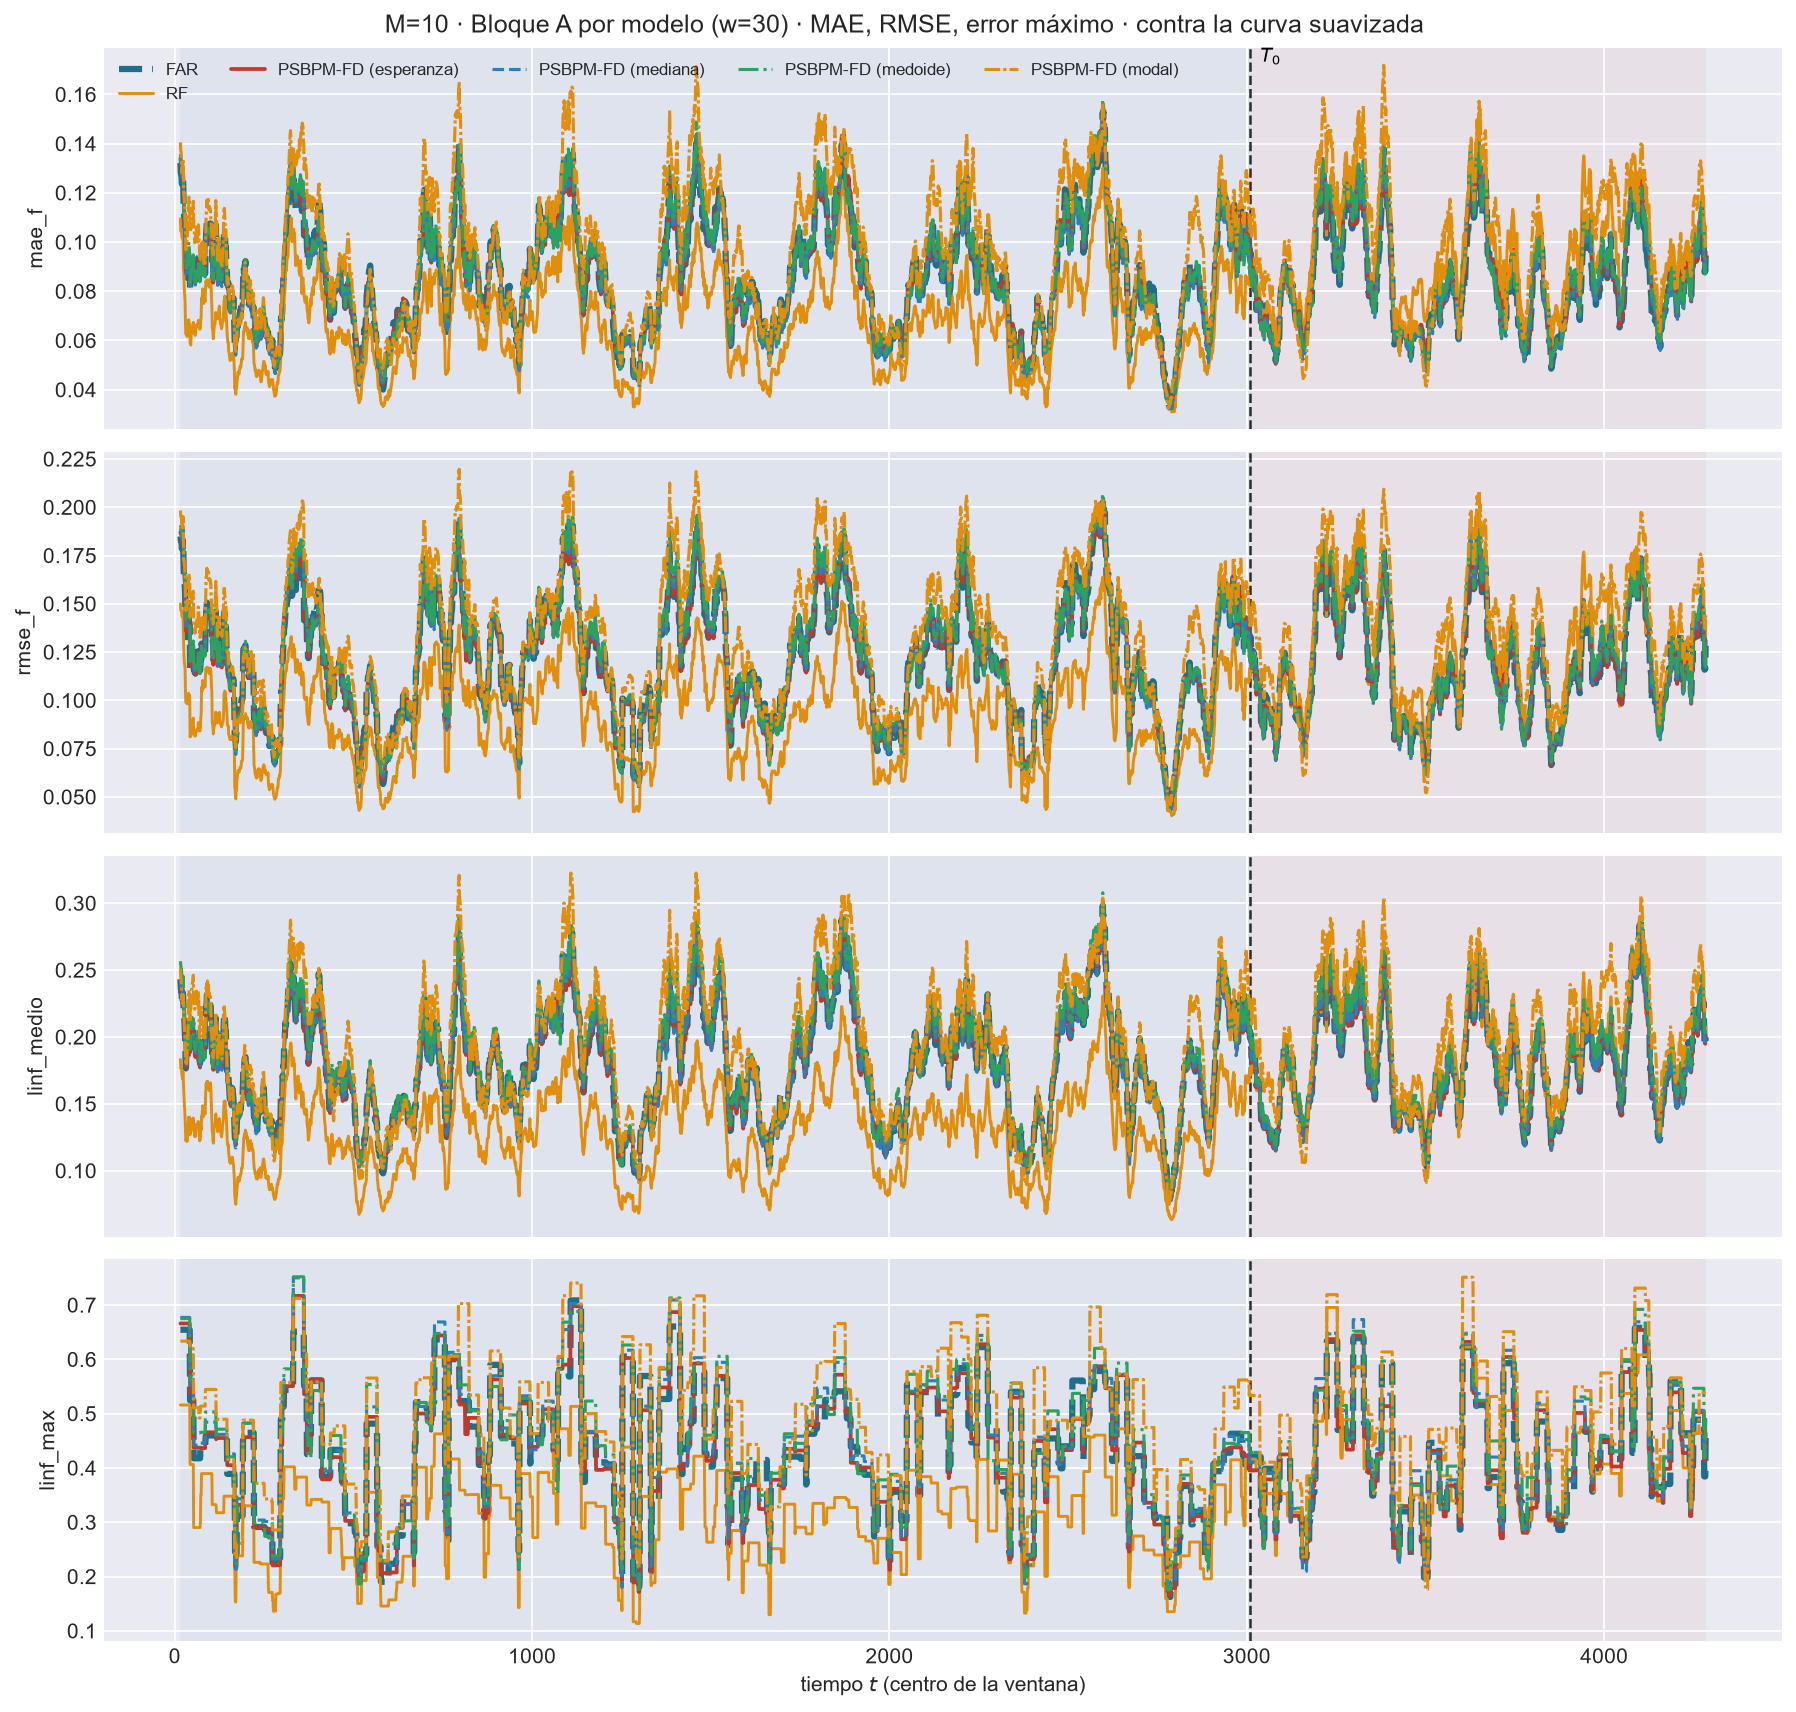
\includegraphics[width=\textwidth,height=0.75\textheight,keepaspectratio]{IMG/aneD_00/aneD_00_78_ventana_bloqueA_modelos_w30_106.png}
\caption{Factor de planta eólico (SMARD). MAE sobre la ventana móvil del bloque de prueba ($M = 10$, $w = 30$).}
\label{fig:aneD_78_ventana_bloqueA_modelos_w30_106}
\end{figure}

\begin{figure}[H]
\centering
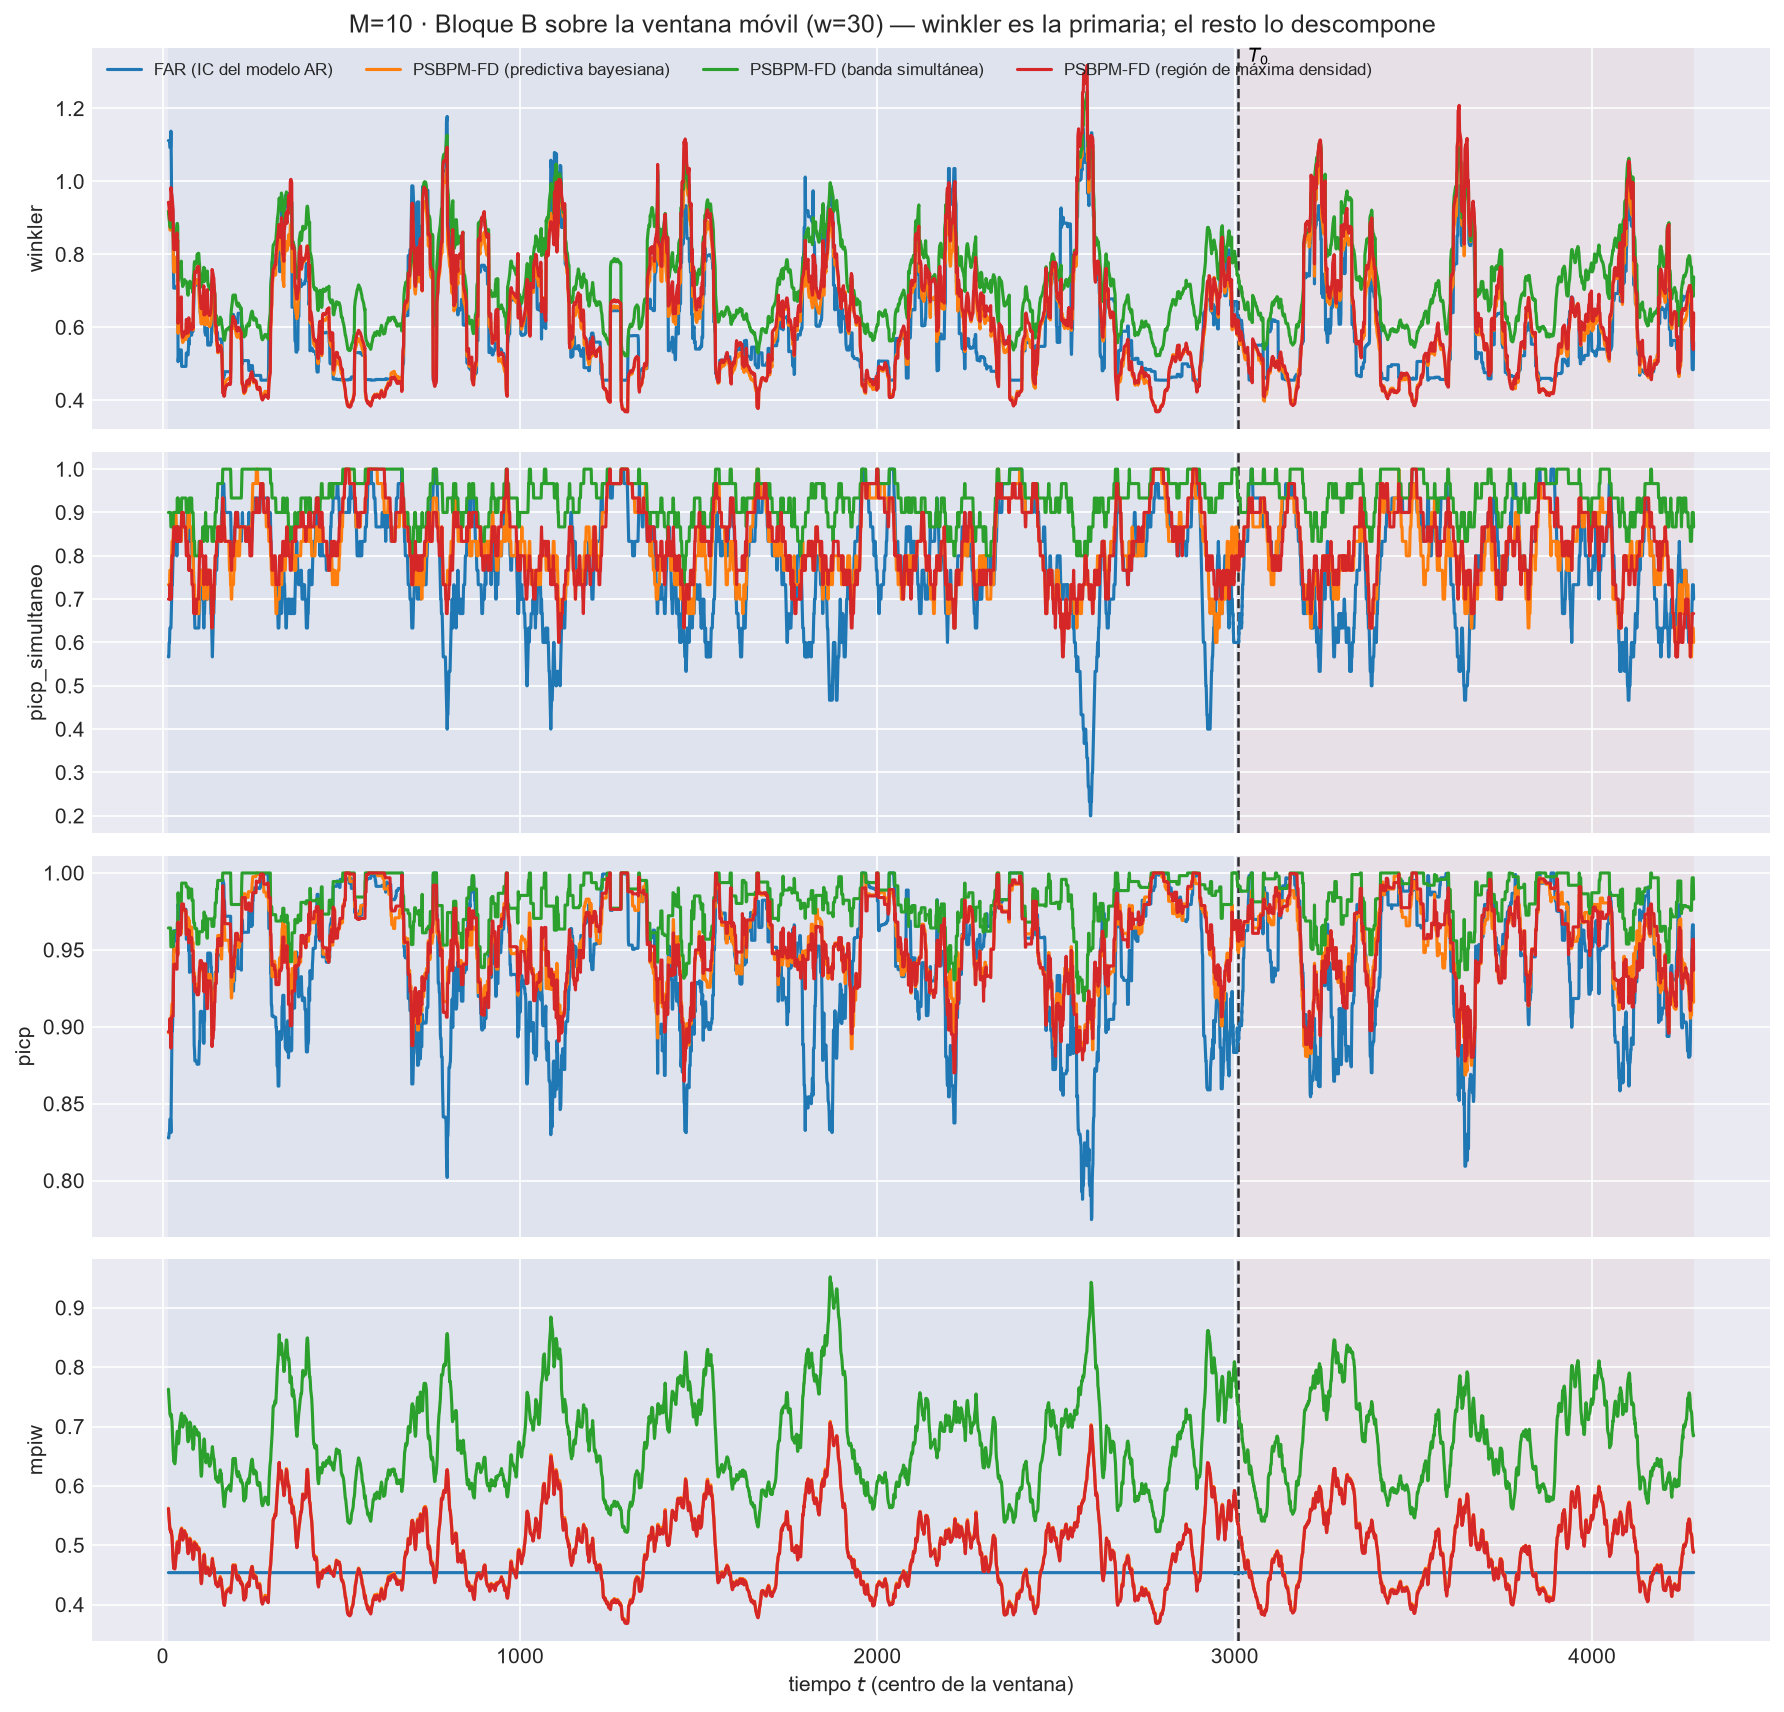
\includegraphics[width=\textwidth,height=0.75\textheight,keepaspectratio]{IMG/aneD_00/aneD_00_81_ventana_bloqueB_w30_106.png}
\caption{Factor de planta eólico (SMARD). Winkler sobre la ventana móvil del bloque de prueba ($M = 10$, $w = 30$).}
\label{fig:aneD_81_ventana_bloqueB_w30_106}
\end{figure}

\begin{figure}[H]
\centering
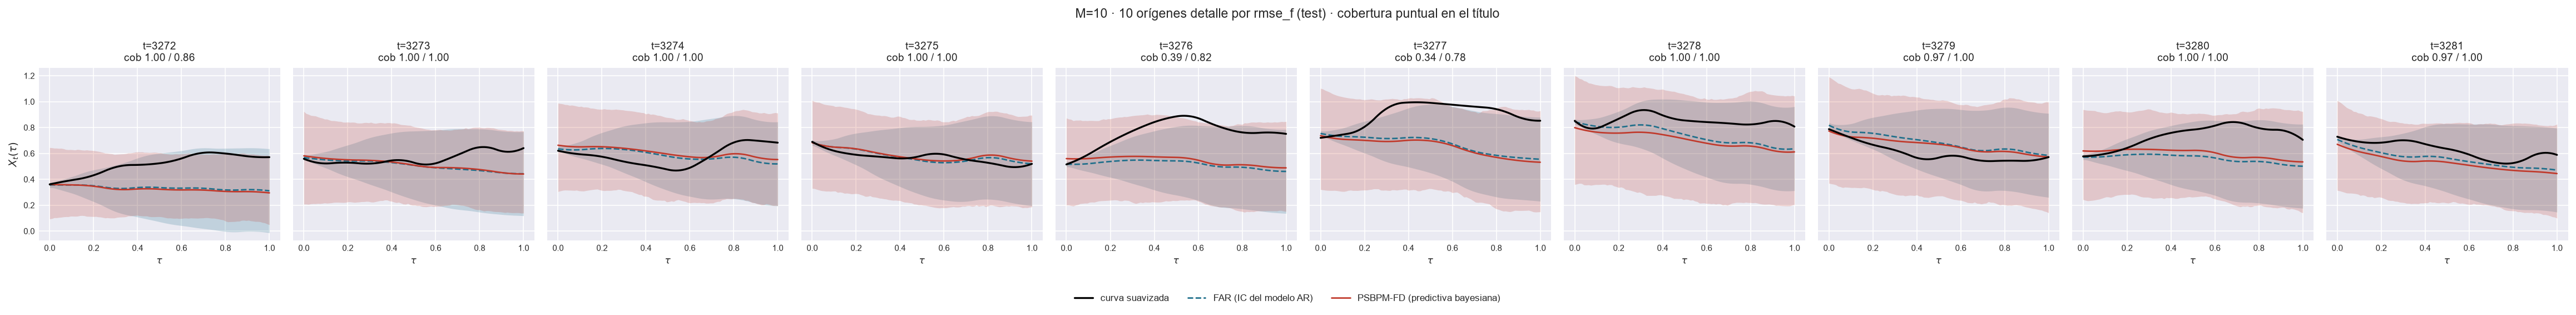
\includegraphics[width=\textwidth,height=0.75\textheight,keepaspectratio]{IMG/aneD_00/aneD_00_79_ic_contraste_detalle_106.png}
\caption{Factor de planta eólico (SMARD). Bandas equi-colas y del FAR en la ventana de detalle ($M = 10$).}
\label{fig:aneD_79_ic_contraste_detalle_106}
\end{figure}

\begin{figure}[H]
\centering
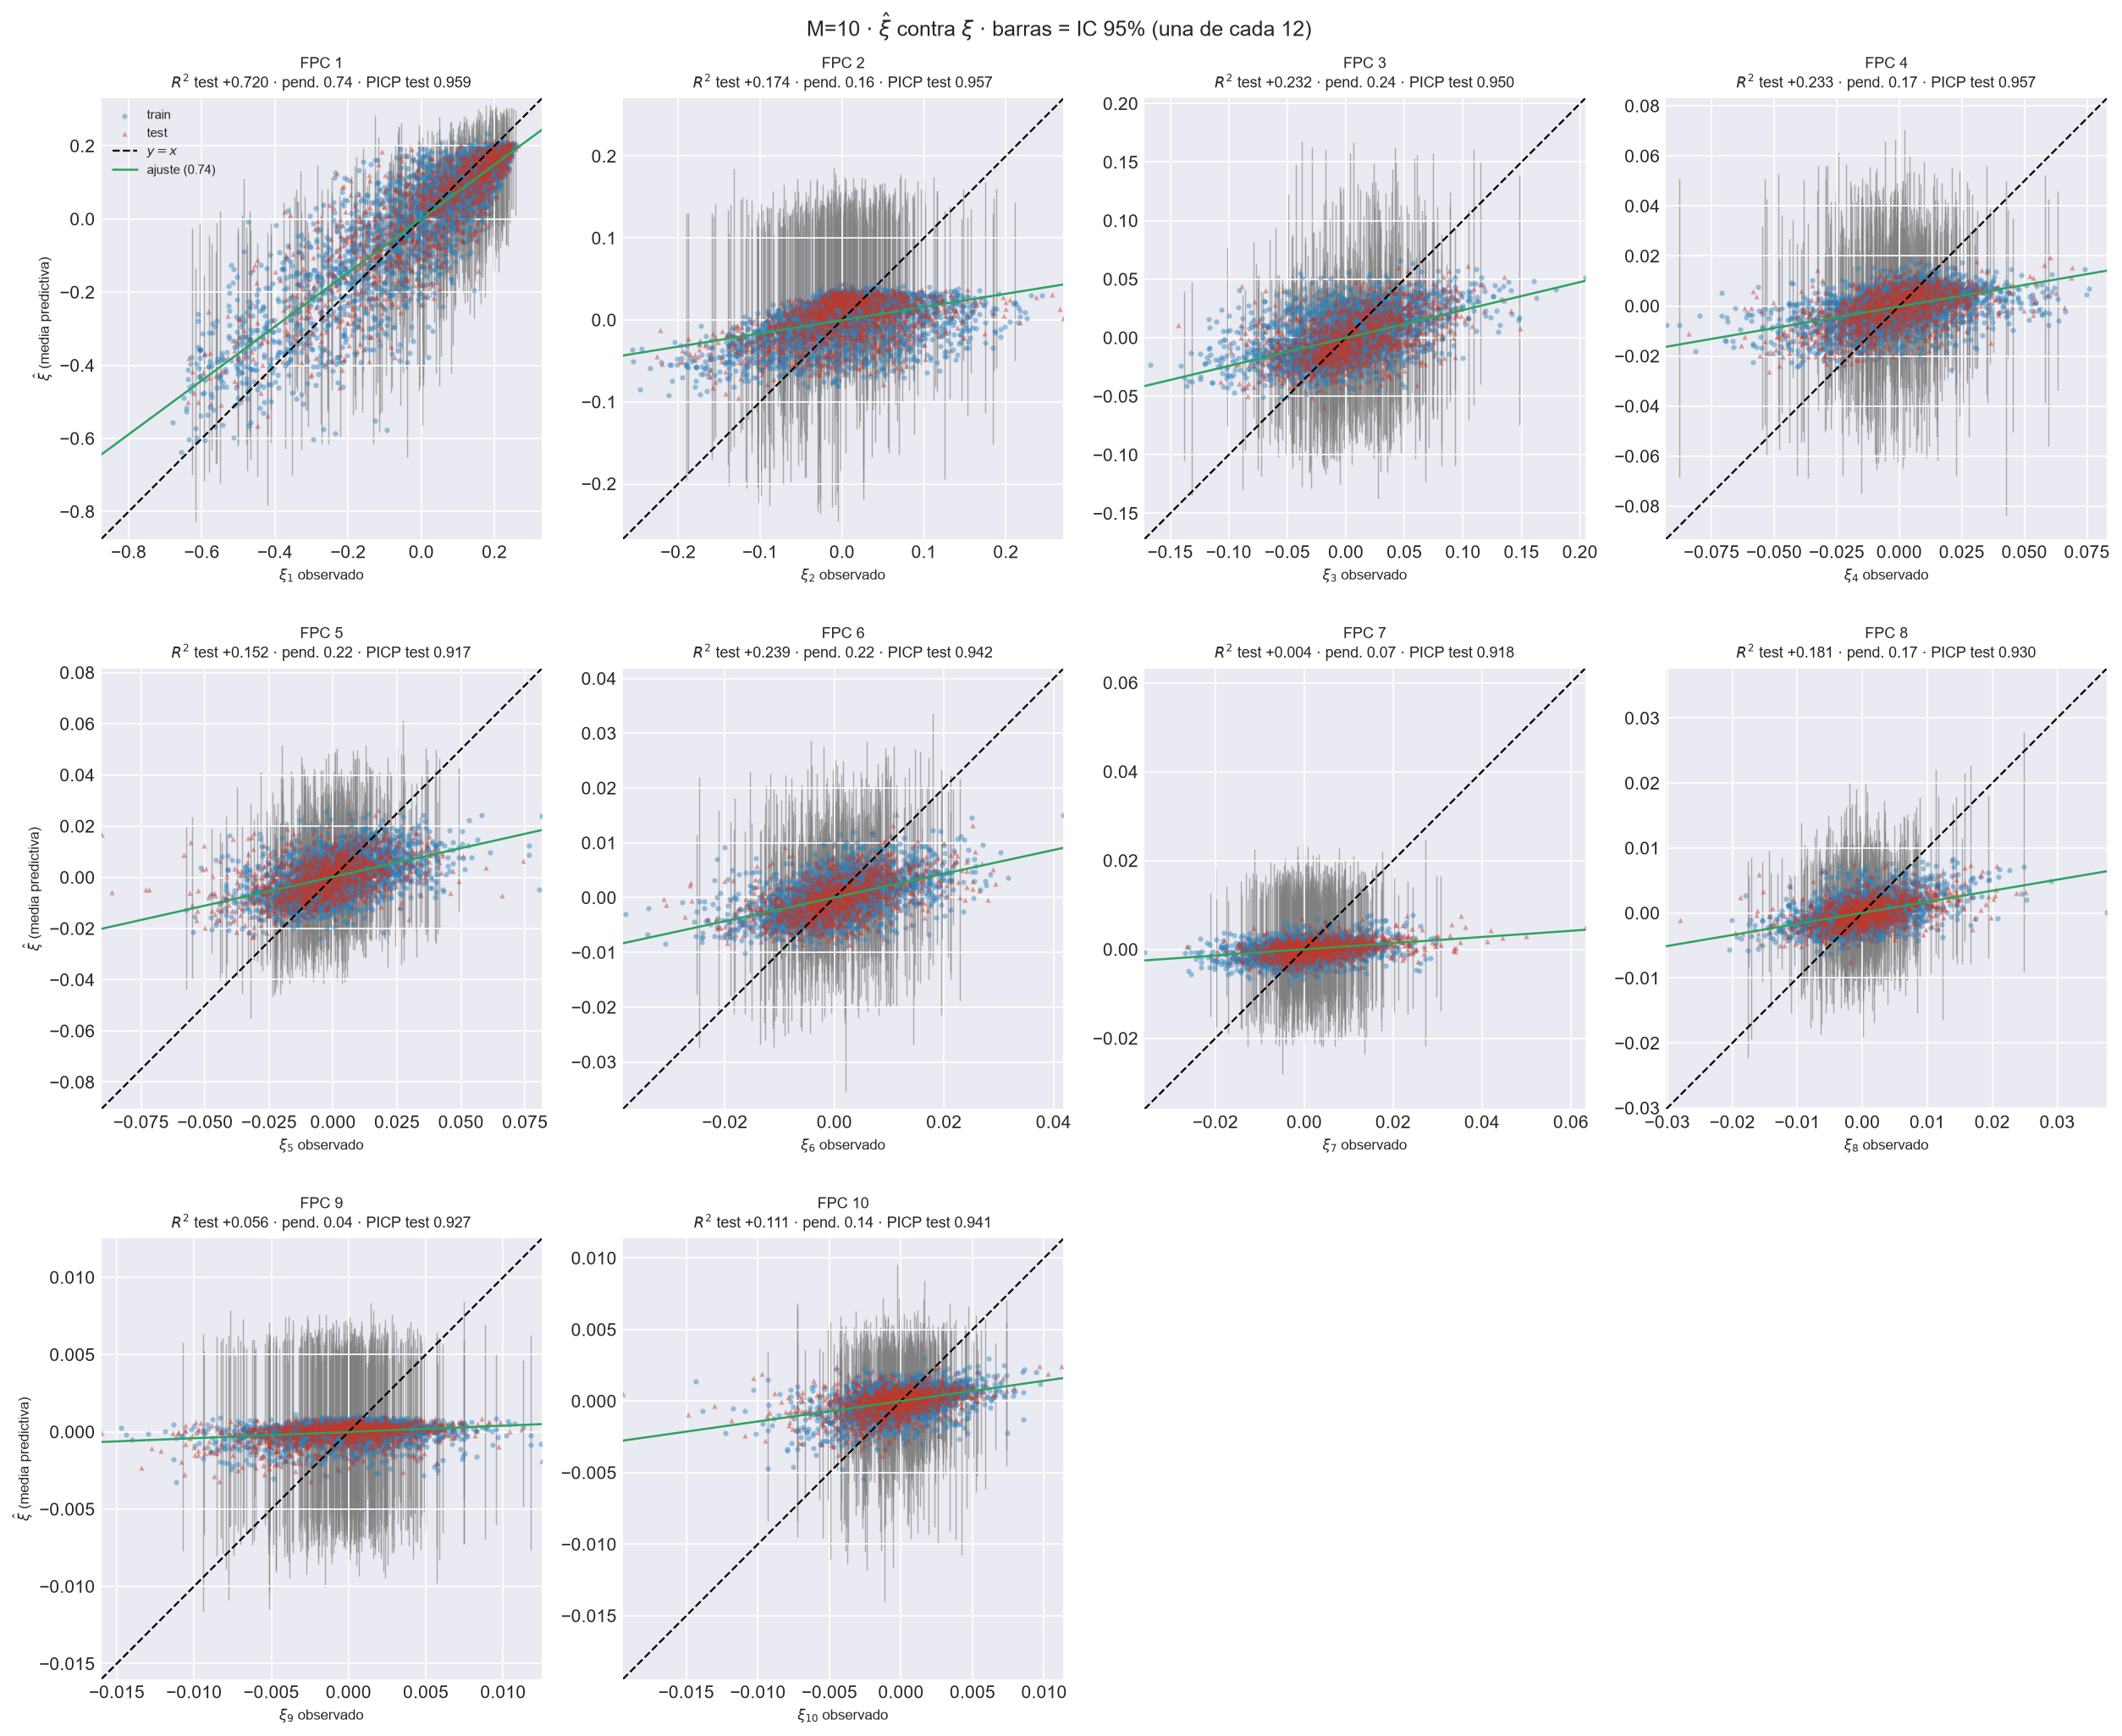
\includegraphics[width=\textwidth,height=0.75\textheight,keepaspectratio]{IMG/aneD_00/aneD_00_94_scores_dispersion_vs_real_106.png}
\caption{Factor de planta eólico (SMARD). Dispersión estimada de cada score frente a la observada ($M = 10$).}
\label{fig:aneD_94_scores_dispersion_vs_real_106}
\end{figure}

\subsection{Volatilidad realizada de BTCUSDT}
\label{aneD_00_05_107}

\begin{figure}[H]
\centering
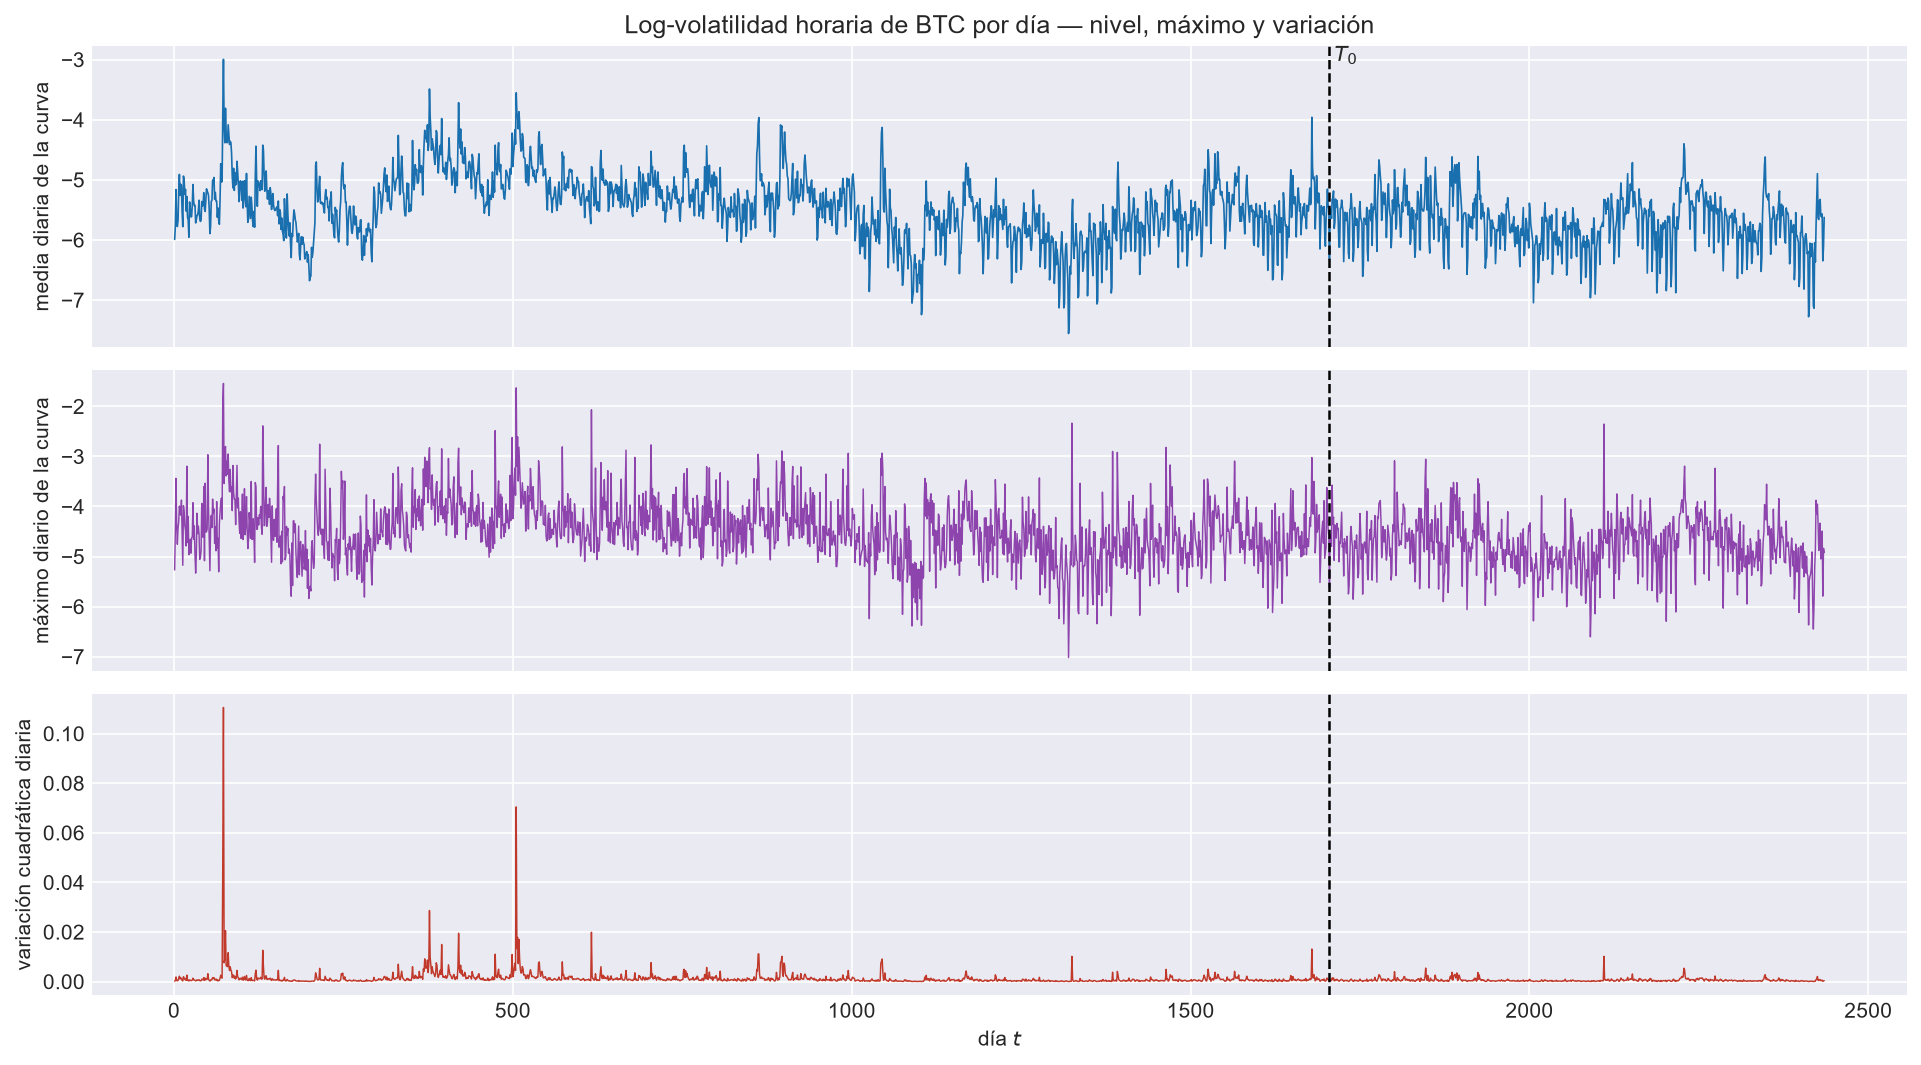
\includegraphics[width=\textwidth,height=0.75\textheight,keepaspectratio]{IMG/aneD_00/aneD_00_04_serie_diaria_107.png}
\caption{Volatilidad realizada de BTCUSDT. Serie diaria.}
\label{fig:aneD_04_serie_diaria_107}
\end{figure}

\begin{figure}[H]
\centering
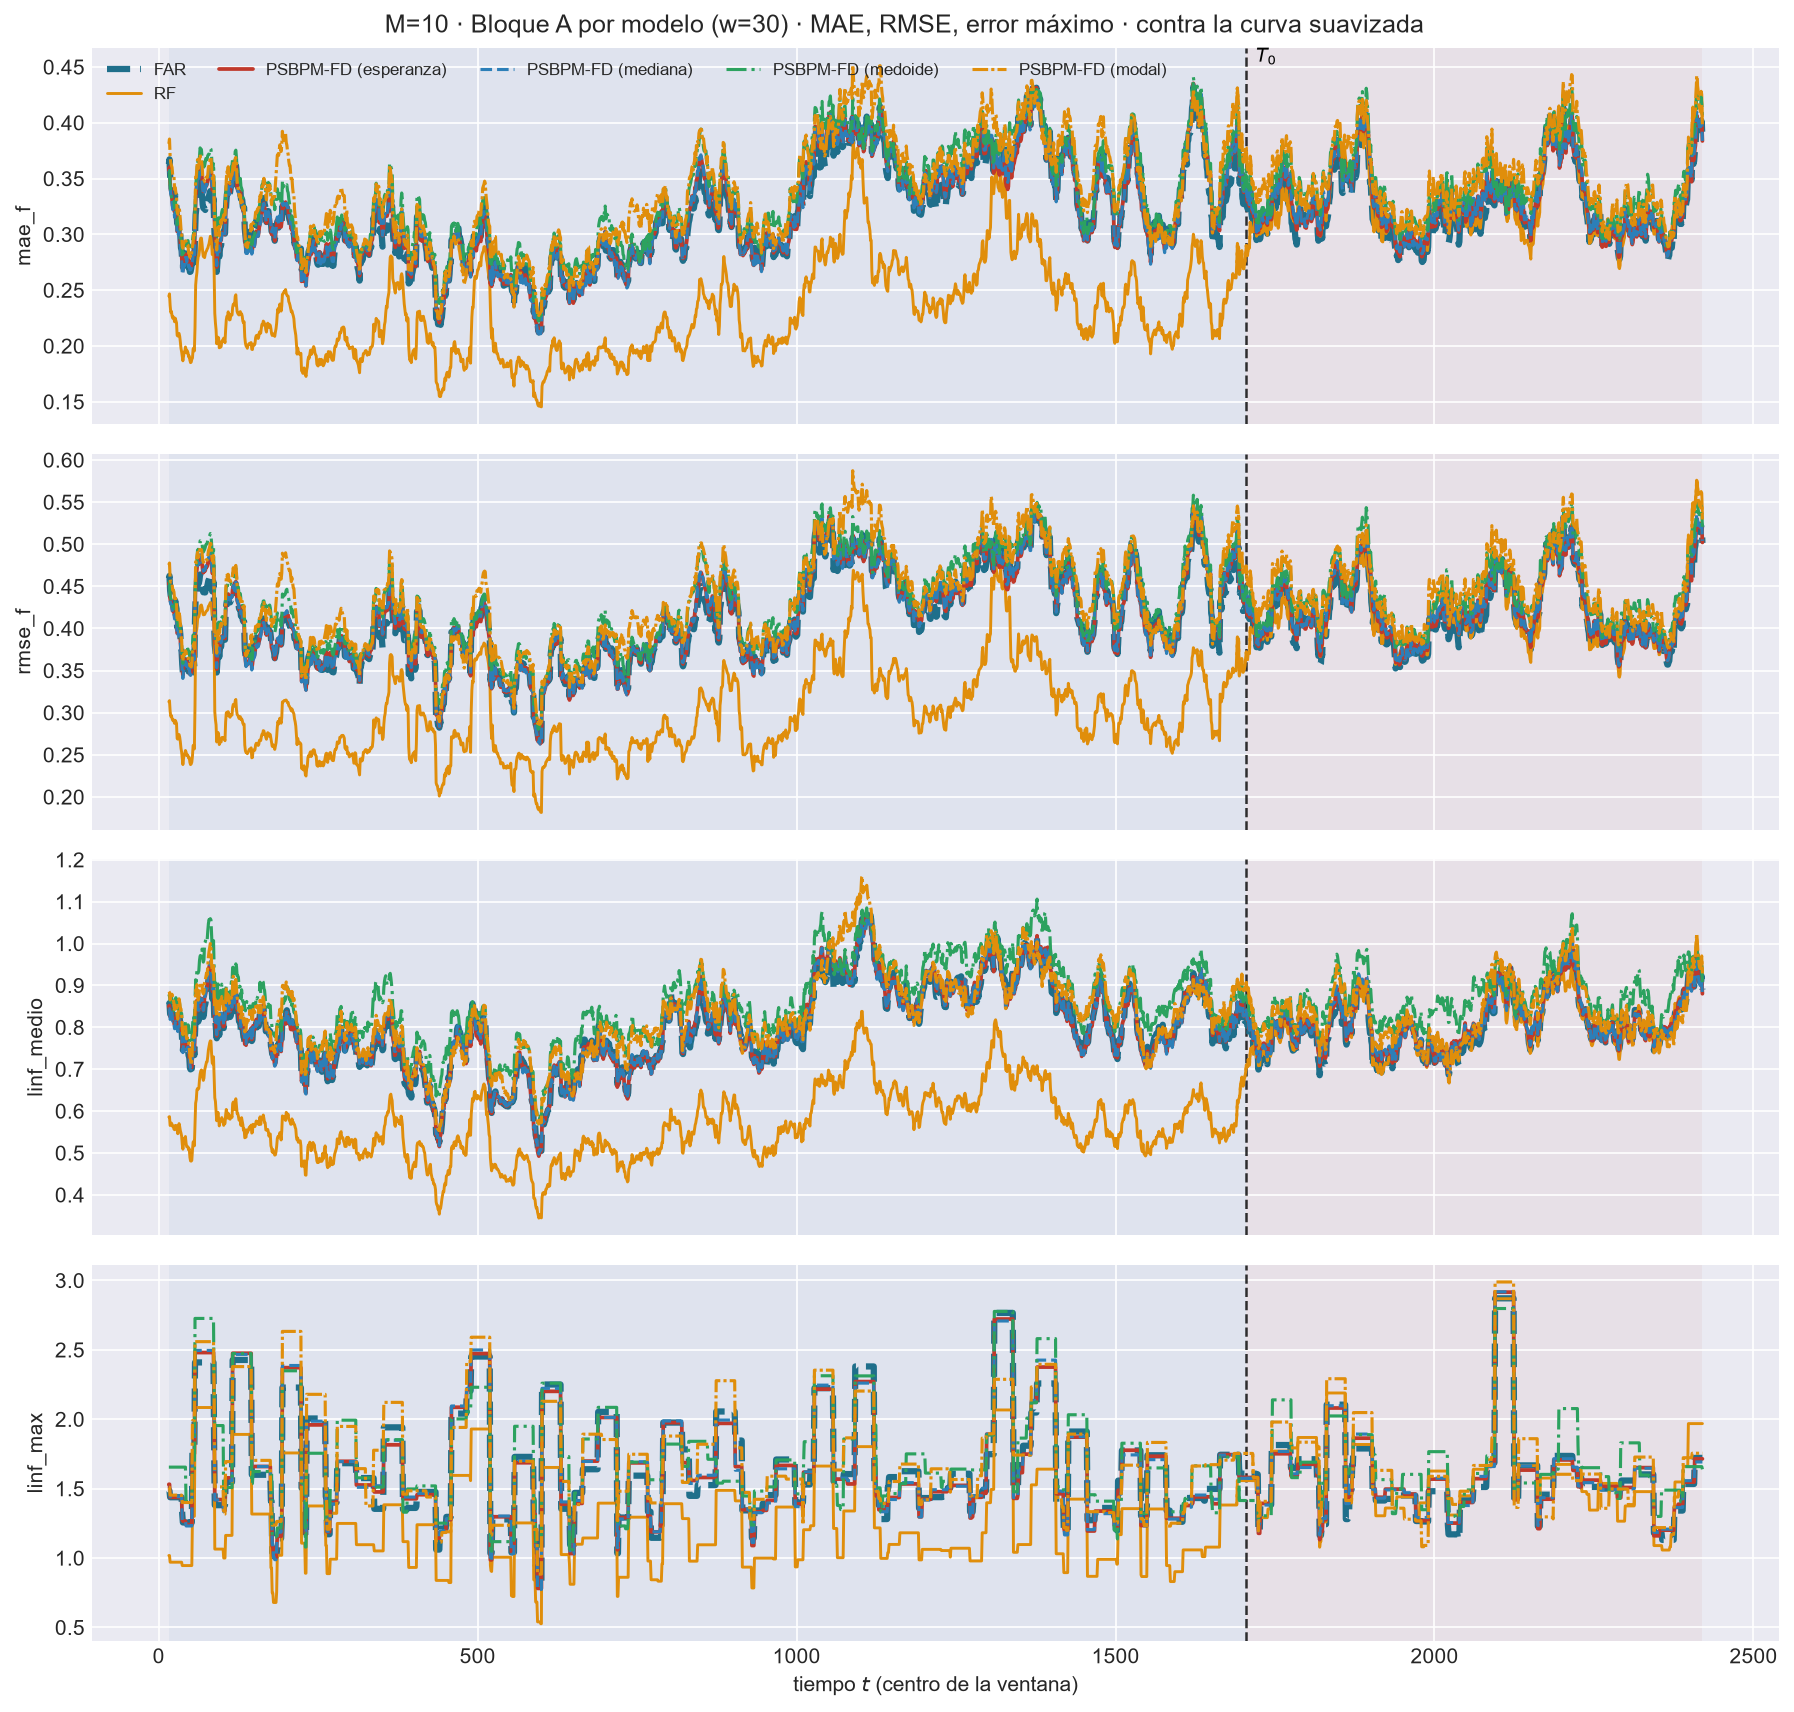
\includegraphics[width=\textwidth,height=0.75\textheight,keepaspectratio]{IMG/aneD_00/aneD_00_78_ventana_bloqueA_modelos_w30_107.png}
\caption{Volatilidad realizada de BTCUSDT. MAE sobre la ventana móvil del bloque de prueba ($M = 10$, $w = 30$).}
\label{fig:aneD_78_ventana_bloqueA_modelos_w30_107}
\end{figure}

\begin{figure}[H]
\centering
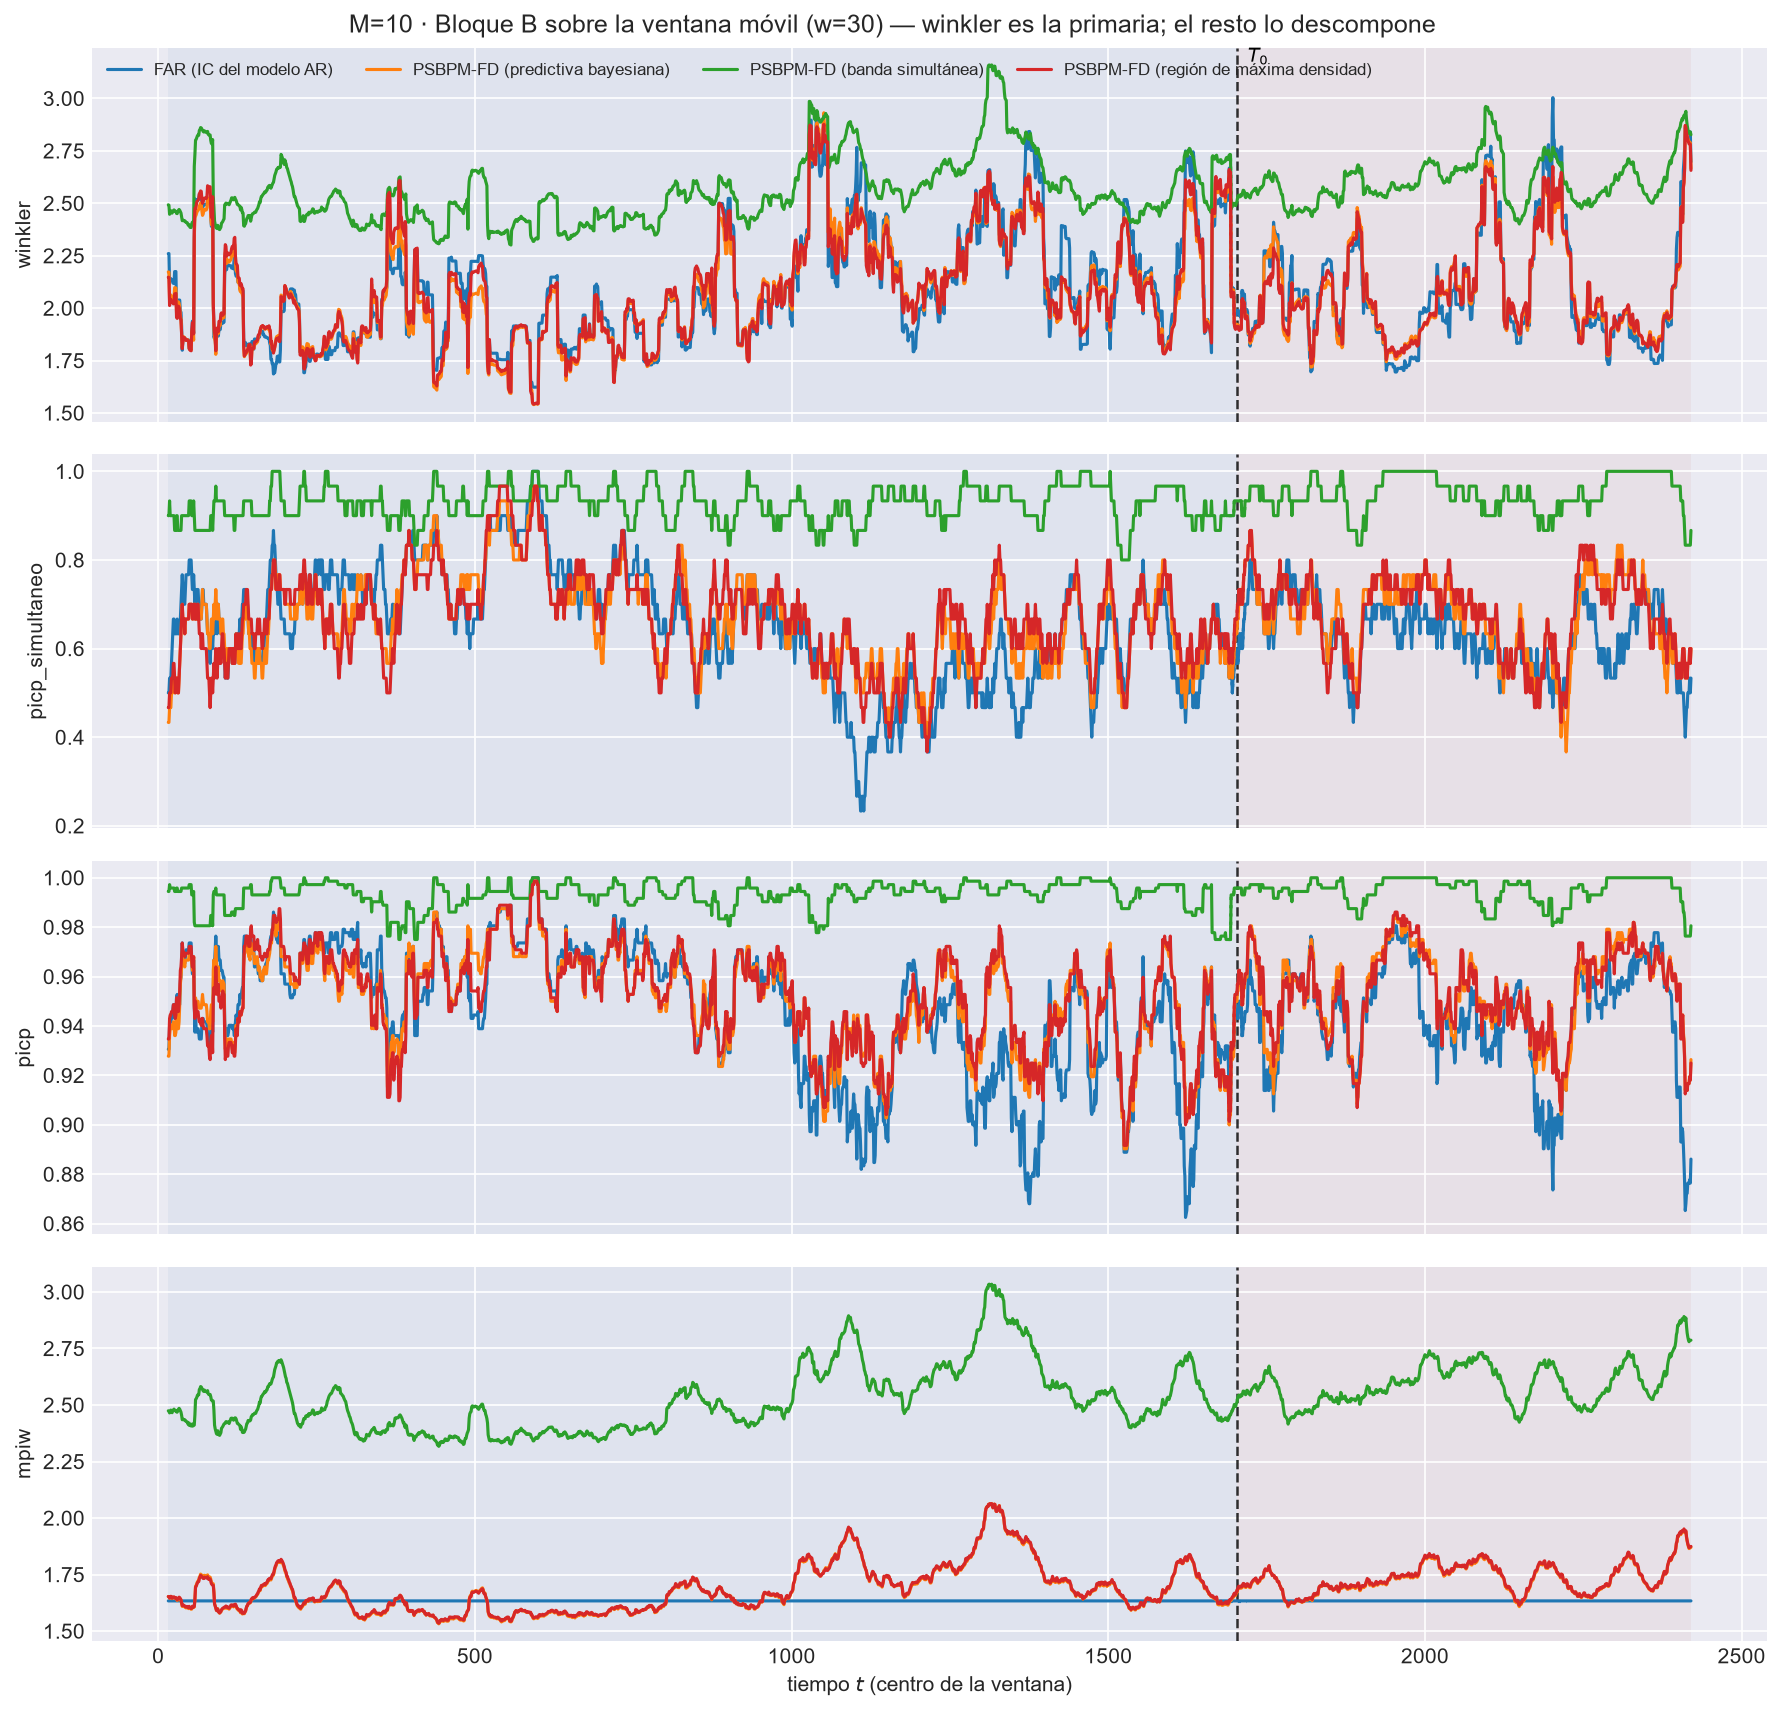
\includegraphics[width=\textwidth,height=0.75\textheight,keepaspectratio]{IMG/aneD_00/aneD_00_81_ventana_bloqueB_w30_107.png}
\caption{Volatilidad realizada de BTCUSDT. Winkler sobre la ventana móvil del bloque de prueba ($M = 10$, $w = 30$).}
\label{fig:aneD_81_ventana_bloqueB_w30_107}
\end{figure}

\begin{figure}[H]
\centering
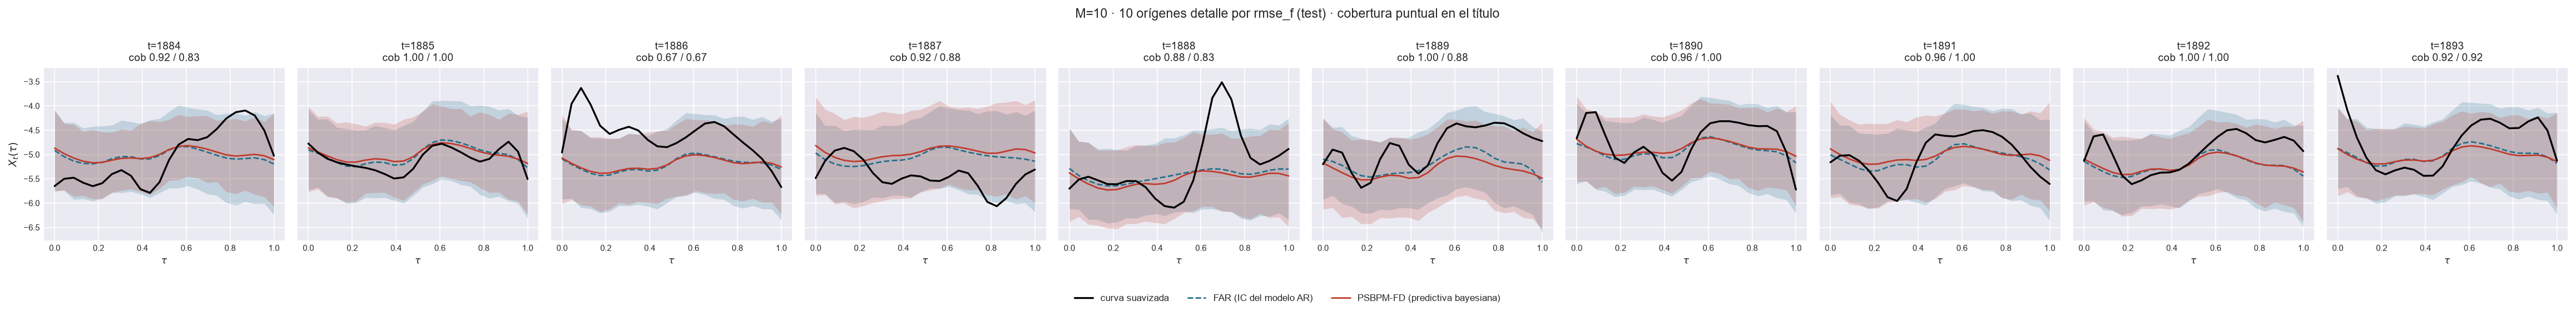
\includegraphics[width=\textwidth,height=0.75\textheight,keepaspectratio]{IMG/aneD_00/aneD_00_79_ic_contraste_detalle_107.png}
\caption{Volatilidad realizada de BTCUSDT. Bandas equi-colas y del FAR en la ventana de detalle ($M = 10$).}
\label{fig:aneD_79_ic_contraste_detalle_107}
\end{figure}

\begin{figure}[H]
\centering
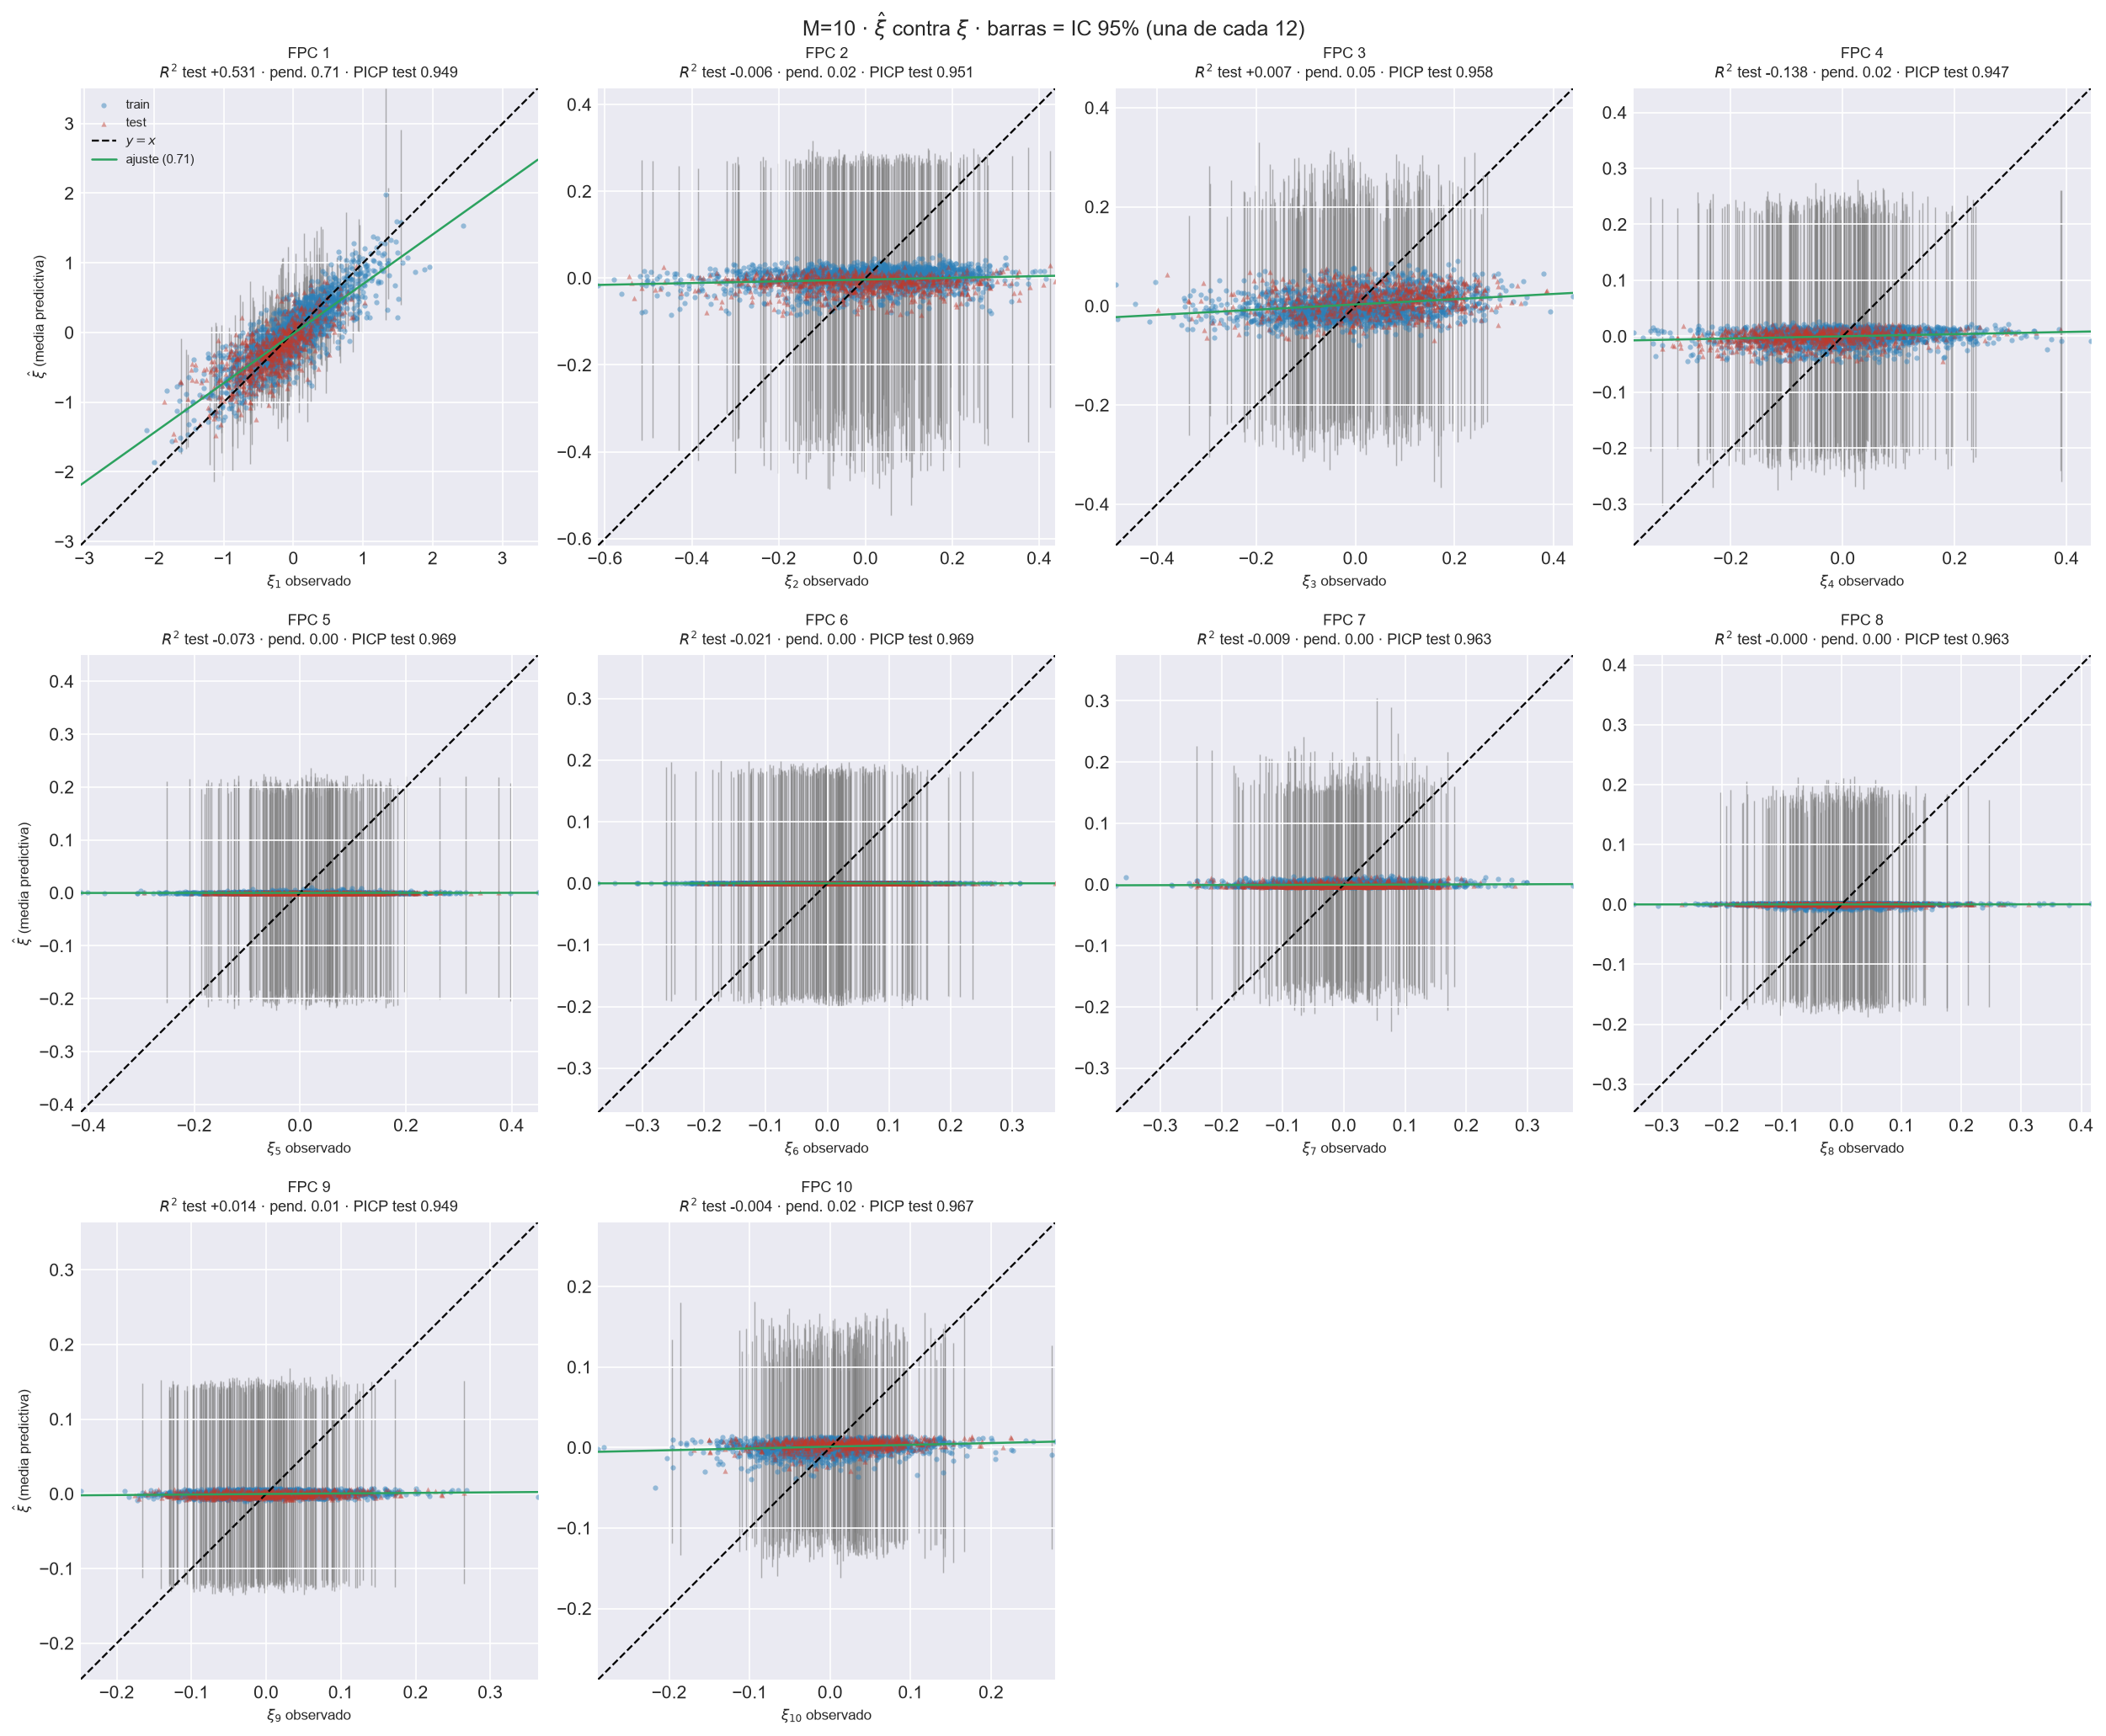
\includegraphics[width=\textwidth,height=0.75\textheight,keepaspectratio]{IMG/aneD_00/aneD_00_94_scores_dispersion_vs_real_107.png}
\caption{Volatilidad realizada de BTCUSDT. Dispersión estimada de cada score frente a la observada ($M = 10$).}
\label{fig:aneD_94_scores_dispersion_vs_real_107}
\end{figure}

